% !TEX encoding = IsoLatin
\documentclass[spanish,a4paper,12pt]{article}
\usepackage[utf8]{inputenc}
\usepackage[T1]{fontenc}
\usepackage[es-noshorthands]{babel}
\usepackage[dvips]{graphicx}
\usepackage{graphicx}
\usepackage{subcaption}
\usepackage{amsmath,amssymb,amsthm}
\usepackage{mathrsfs}
\usepackage{arydshln}
\usepackage{jgn}
\usepackage{fancyheadings}
\usepackage[thinlines,thiklines]{easybmat}
\usepackage[export]{adjustbox}
\usepackage{babel}
\decimalpoint

\usepackage{pdfpages}

% IMAGEBOX
\def\imagebox#1#2{\vtop to #1{\null\hbox{#2}\vfill}}


\usepackage[top=25mm,left=20mm,body={170mm,255mm}]{geometry}
\usepackage{hyperref}

\usepackage[scaled]{beramono}

\usepackage[framed,numbered,autolinebreaks,useliterate]{mcode}

\usepackage{upquote}
\usepackage{xcolor}
\usepackage{listings}
\usepackage{caption}


\lstset{language=Matlab,breaklines=false,numbers=none}

\lstset{literate=
  {á}{{\'a}}1 {é}{{\'e}}1 {í}{{\'i}}1 {ó}{{\'o}}1 {ú}{{\'u}}1
  {Á}{{\'A}}1 {É}{{\'E}}1 {Í}{{\'I}}1 {Ó}{{\'O}}1 {Ú}{{\'U}}1
  {à}{{\`a}}1 {è}{{\`e}}1 {ì}{{\`i}}1 {ò}{{\`o}}1 {ù}{{\`u}}1
  {À}{{\`A}}1 {È}{{\'E}}1 {Ì}{{\`I}}1 {Ò}{{\`O}}1 {Ù}{{\`U}}1
  {ä}{{\"a}}1 {ë}{{\"e}}1 {ï}{{\"i}}1 {ö}{{\"o}}1 {ü}{{\"u}}1
  {Ä}{{\"A}}1 {Ë}{{\"E}}1 {Ï}{{\"I}}1 {Ö}{{\"O}}1 {Ü}{{\"U}}1
  {â}{{\^a}}1 {ê}{{\^e}}1 {î}{{\^i}}1 {ô}{{\^o}}1 {û}{{\^u}}1
  {Â}{{\^A}}1 {Ê}{{\^E}}1 {Î}{{\^I}}1 {Ô}{{\^O}}1 {Û}{{\^U}}1
  {?}{{\oe}}1 {?}{{\OE}}1 {æ}{{\ae}}1 {Æ}{{\AE}}1 {ß}{{\ss}}1
  {?}{{\H{u}}}1 {?}{{\H{U}}}1 {?}{{\H{o}}}1 {?}{{\H{O}}}1
  {ç}{{\c c}}1 {Ç}{{\c C}}1 {ø}{{\o}}1 {å}{{\r a}}1 {Å}{{\r A}}1
  {?}{{\EUR}}1 {£}{{\pounds}}1
}

 


 \hypersetup{
 colorlinks,
 breaklinks=true,backref,bookmarksnumbered=true,
 pdfauthor={GMC},
 pdftitle={Session 3. Topic 1. Finite element models for an elastic 1D bar}}
% \usepackage{subfigure}


\selectspanish
\title{\vspace*{-4ex}
	\bf\normalsize
	Métodos Computacionales en Ingeniería Civil\\
	\Large
	Session \#3, Topic 1.\\
	Finite element models for an elastic 1D bar\\[3ex]
%	\parbox[c]{0.4\textwidth}{%
%%	\includegraphics[width=0.45\linewidth]{sc-nh-post/nh-neoh-0.png}
%%	\includegraphics[width=0.45\linewidth]{sc-nh-post/nh-neoh-1.png}%
%	}%
%	\parbox[c]{0.6\textwidth}{%
	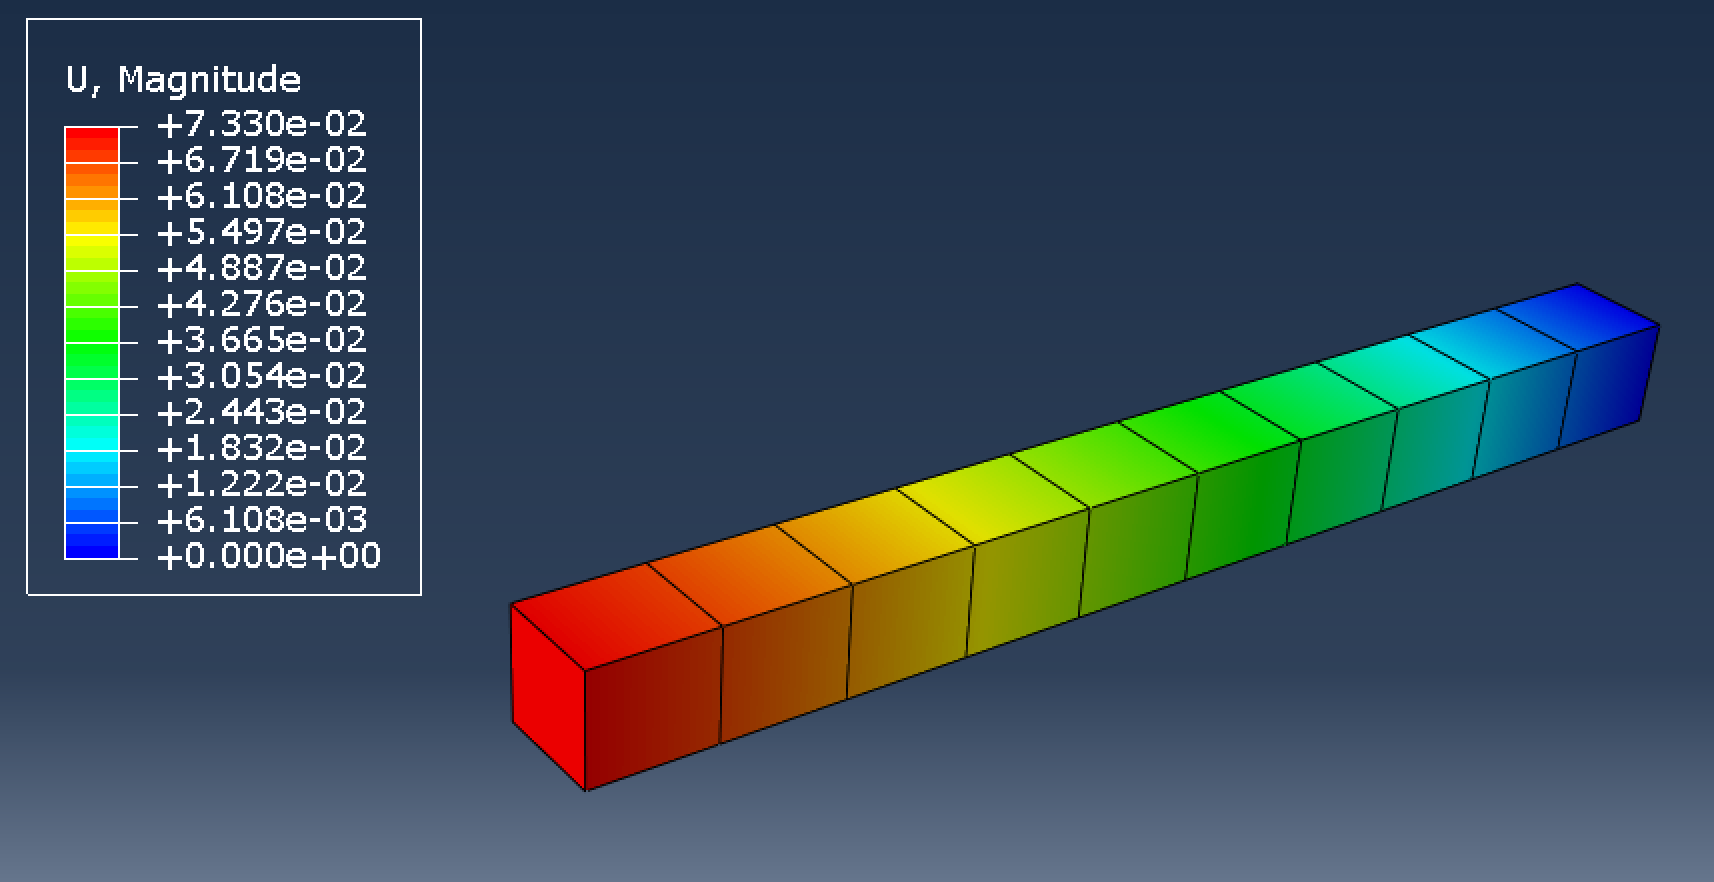
\includegraphics[width=0.65\linewidth]{figuras/barra_portada.png}%
	%}
	}
\author{%José M.ª Goicolea, Pedro Navas, Juan José Arribas, A. Cámara\\
        {\small\sc 
	Grupo de Mecánica Computacional, ETSICCP, UPM}}
\date{15-16 de febrero de 2023}


\begin{document}

\pagestyle{fancy}
\lhead[\fancyplain{}{\thepage}]{\fancyplain{}{\rightmark}}
\rhead[\fancyplain{}{\leftmark}]{\fancyplain{}{\thepage}}
\cfoot[\fancyplain{\thepage}{}]{\fancyplain{\thepage}{}}

\renewcommand{\sectionmark}[1]{\markright{\sf Aptdo.\ \thesection. #1}{}}
\renewcommand*\lstlistingname{Código}

\maketitle

\tableofcontents

\addtocontents{toc}{\protect\hrule}

\clearpage

\section{Objetives}
\label{sec:objetivos}

This session focuses on the development of a Finite Element (FE) code in the programming language \texttt{Python} that can solve a 1D elastic problem in which a bar is subject to axial loading. In addition, the Appendix includes the same code in the programming language \texttt{Matlab/Octave}. We adopt the following assumptions and conditions:
\begin{enumerate}
	\item
	The students have the basic theoretical background regarding the construction of elementary stiffness matrices, which should be coded by the studentship. 
	\item
	In addition, these elementary matrices will become part of a global system through their assembly, a process that is also known by the students. 
	\item
	In order to solve the system of equations it is necessary to know the boundary conditions of loading and displacements in the problem. These need to be applied to the matricial system developed in \texttt{Python}.
\end{enumerate}

Furthermore, we are going to simulate a 1D bar analogous to that solved in \texttt{Python} using the commercial FE software suite \texttt{Abaqus}. This will help assimilating the basic concepts of pre-processing, analysis and post-processing that will support the following practical sessions. The results obtained with the two methods will be compared with the analytical (exact) solution to the problem, which should be obtained by the student too, using the available plotting tools for this purpose.




\section{Theoretical background and FE discretisation}
\label{sec:teoria}

%\subsection{Governing equations}
\subsection{Governing equations}

The governing equation of a 1D linear elastic bar subject to axial loads is an elliptic differential equation in terms of the along-bar displacement \(u(x)\):

\begin{equation}\label{eq:gov}
\frac{\mathrm{d (A \sigma)}}{\mathrm{d} x} + q(x)
=\frac{\mathrm{d}}{\mathrm{d} x}\left(EA \frac{\mathrm{d} u}{\mathrm{d} x}\right)+q(x)=0
\end{equation}

Where $E$ is the Young's modulus, an elastic parameter that describes its stiffness, $q(x)$ represents the distributed forces along the bar per unit length $x$. The solution to the problem requires finding a displacement distribution \(u(x)\) in the open interval of the length of the bar $(0,L)$ so that the system is in equilibrium considering the boundary conditions defined for the problem.

\subsection{Boundary conditions and volumetric forces}

The possible boundary conditions that we will find in the problem to solve can be summarise d in Fig.~\ref{fig:CC1D}.

\begin{figure}[!htp]
\centering
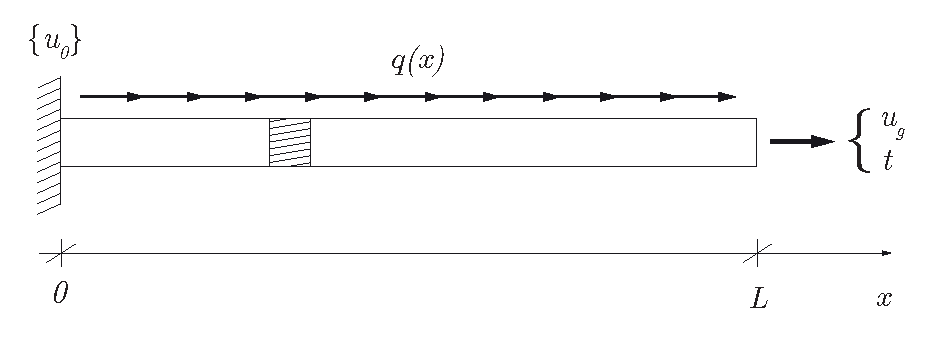
\includegraphics[width=0.8\textwidth]{figuras/1D.pdf}
\caption{Problem definition and boundary conditions.}
\label{fig:CC1D}
\end{figure}

We can find basically two types of boundary conditions:

\begin{itemize}
\item \textit{Type Dirichlet or Essentials}\\
These boundaries are applied to the response field in which we have defined the governing differential equation; in our case this is \(u(x)\) and therefore the Dirichlet boundary conditions refer to ``displacements'' at specific points (usually the ends of the bar):
$$
u(0)=u_0
$$$$
u(L)=u_g
$$
\item \textit{Type Neumann or Naturals}\\
These boundaries are applied to the spatial derivative of the response field in which we have defined the governing differential equation, which considering our case will be:
$$
t= EA \frac{\mathrm{d} u}{\mathrm{d} x} \biggr\rvert_{x=L}
$$
Therefore, these could be considered boundary conditions related to ``forces'' for this problem.

\end{itemize}
On the other hand, we have the \textit{volumetric or distributed forces}, which are those applied to the whole domain of the structure. In Eq.~\eqref{eq:gov} these forces are defined by $q(x)$. In general they depend on the position $x$, but they can also be constant.
An example of these forces in the mechanical problem are those associated with gravity $g$, which depend on the area of the cross-section of the bar $A(x)$ and its density $\rho(x)$ that can also be variable along the length:
\begin{equation*}
q(x) =A(x) \rho(x) g
\end{equation*}
In this session, $q(x)$ will be a function of $x$ that is given to represent a load per unit length in the bar.

\subsection{Strong formulation and analytical solution tothe problem}
\label{sec:analitica}
Eq.~\eqref{eq:gov} is the strong formulation of the problem. It is called like this because its solution is satisfied at any point of the domain $(0,L)$. 

As we can see, this strong formulation involves a second derivative of \(u(x)\), which implies that his field has to be differentiable of order two with respect to $x$.\\

The solution of the strong formulation leads to an analytical solution that is exact if we assume that the area $A$ and the Young's modulus $E$ are constant in the entire bar. We start with the strong formulation of the displacement field between an arbitrary point $y\in(0,L)$ and the end of the bar at $x=L$:
\begin{eqnarray}
A \int_y^L \frac{\mathrm{d \sigma}}{\mathrm{d} x} \mathrm{d} x &=& -\int_y^L  q(x) \mathrm{d} x \\
\sigma(L)-\sigma(y) &=& -\frac{1}{A}\int_y^L  q(x) \mathrm{d} x 
\end{eqnarray}

Adopting the definition of the 1D linear elastic constitutive equation, $\sigma = E\, \dr u/\dr x$:
\begin{equation}
E \frac{\mathrm{d} u(y)}{\mathrm{d} y} = E \frac{\mathrm{d} u}{\mathrm{d} x} \biggr\rvert_{x=L}  +\frac{1}{A}\int_y^L  q(x) \mathrm{d} x 
\end{equation}
Again, we integrate between the start of the bar at $x=0$ and a point $z\in(0,L)$:
\begin{equation}
\int_0^z E \frac{\mathrm{d} u(y)}{\mathrm{d} y} \mathrm{d} y = \int_0^z \left( E \frac{\mathrm{d} u}{\mathrm{d} x} \biggr\rvert_{x=L}  +\frac{1}{A}\int_y^L  q(x) \mathrm{d} x \right) \mathrm{d} y
\end{equation}

Assuming that the derivative of $u$ with respect to $x$ is known at $x=L$ (Neumann boundary condition), the result of the integral is:
\begin{equation}
E u(z) - E u(0) = E \frac{\mathrm{d} u}{\mathrm{d} x} \biggr\rvert_{x=L} z + \frac{1}{A}\int_0^z\int_y^L  q(x) \mathrm{d} x \mathrm{d} y
\end{equation}
Therefore, the solution of $u(z)$ is:
\begin{equation}\label{eq:anal}
u(z)  = u(0) +  \frac{\mathrm{d} u}{\mathrm{d} x} \biggr\rvert_{x=L} z  +\frac{1}{EA}\int_0^z\int_y^L  q(x) \mathrm{d} x \mathrm{d} y
\end{equation}

The analytical solution of Eq.~\eqref{eq:anal} depends on two constants that need to be determined by imposing the boundary conditions at the two ends of the bar. In our case these are: $u(0) $ and $\dr u / \dr x |_{x=L}$, which correspond to types Dirichlet and Neumann, respectively. In a different case in which the boundary condition at the free end is not natural but based on displacements at $x=L$, the term $\dr u / \dr x |_{x=L}$ can be obtained by imposing $z=L$, with $u(L)$ being given.

For the specific scenario in which the boundary conditions refer to a bar fixed at the left end and with given axial load at the right end; $u(0)=0$ and $EA\dr u/\dr x|_{L}=P$ (load $P$ at $x=L$). And if the distributed axial load is linear with $x$ so that $q(x)=q_{0}+rx$, the analytical expression is:
\begin{equation}
\begin{split}
	u(x) &= \frac{1}{EA}\bigg[ 
	\big(P+q_{0}L+r\frac{L^{2}}{2}\big)x - \big(q_{0}\frac{x^{2}}{2}+r\frac{x^{3}}{6}\big) \bigg]
	\\
	\sigma(x) = E\frac{\dr u}{\dr x}
	&=  \frac{1}{A}\bigg[ 
	P+q_{0}(L-x)+\frac{r}{2}(L^{2}-x^{2}) \bigg]
\end{split}
\label{eq:analitica}
\end{equation}

Considering the hypothesis made, we can only obtain analytical expressions for relatively simple distributions of $E(x)$ and $q(x)$, but not for more complex situations. The latter can be treated numerically in a simpler way, using the weak formulation of the FE method, although the result is generally not exact. 

\subsection{Weak formulation}
\label{sec:debil}

The weak formulation is obtained by multiplying the strong formulation with arbitrary weights $w(x)$ that is then integrated in the domain:
\begin{equation}\label{eq:debil}
\int_{0}^{L} w \frac{\mathrm{d}}{\mathrm{d} x}\left(EA \frac{\mathrm{d} u}{\mathrm{d} x}\right) \mathrm{d} x+\int_{0}^{L} w q \mathrm{d} x=0
\end{equation}

Integrating by parts the first term:

\begin{align}\label{eq:partes}
\frac{\mathrm{d}}{\mathrm{d} x}\left[w \cdot EA \frac{\mathrm{d} u}{\mathrm{d} x}\right] &=\frac{\mathrm{d} w}{\mathrm{d} x} \cdot EA \frac{\mathrm{d} u}{\mathrm{d} x} \quad+w \cdot \frac{\mathrm{d}}{\mathrm{d} x}\left(EA \frac{\mathrm{d} u}{\mathrm{d} x}\right) \nonumber\\
\left[w \cdot EA \frac{\mathrm{d} u}{\mathrm{d} x}\right]_{0}^{L}-\int_{0}^{L} \frac{\mathrm{d} w}{\mathrm{d} x} \cdot EA \frac{\mathrm{d} u}{\mathrm{d} x} \mathrm{d} x &=\int_{0}^{L} w \cdot \frac{\mathrm{d}}{\mathrm{d} x}\left(EA \frac{\mathrm{d} u}{\mathrm{d} x}\right) \mathrm{d} x
\end{align}

we obtain the following result by substituting the Eq.~\eqref{eq:debil}:
\begin{equation}\label{eq:debil1}
\int_{0}^{L} \frac{\mathrm{d} w}{\mathrm{d} x} \cdot EA \frac{\mathrm{d} u}{\mathrm{d} x} \mathrm{d} x=\int_{0}^{L} w q \,\mathrm{d} x+w(L) t_{L}-w(0) t_{0}
\end{equation}
where $t_{L}$ y $t_{0}$ are the natural boundary conditions, which physically correspond to the forces applied at the two ends of the structure.

If an essential boundary condition of imposed or fixed (zero) displacement is applied at the end $x=0$ the weighting function is also $w(0)=0$, therefore the last term of Eq.~\eqref{eq:debil1} vanishes.

\subsection{Funciones de forma}
\label{sec:N}
In the FE method an approximation of the unknown displacement field $u(x)$ using the so-called \textit{shape functions} is needed. These functions interpolate the displacement field within the element based on the nodal displacements and have the expression:
\begin{equation}\label{eq:N1}
u(x) \approx u_{h}(x)=\sum_{B=1}^{N_{\text {nod }}} u_{B} N_{B}(x)
\end{equation}

A discrete set of $\left(N_{\text {nod }}\right)$ shape functions $N_{B}(x)$ is used. This implies certain error which in principle is reduced with the more nodes $N_{\text {nod}}$, or increasing the order of the interpolating functions.

The Galerkin method is the most common one to define the weighting functions $w(x)$ and it is one that will be used in this session. This method proposes using the same weighting functions as the shape functions used to interpolate $u(x)$:
\begin{equation}\label{eq:N2}
w(x) \approx w_{h}(x)=\sum_{A=1}^{N_{\mathrm{nod}}} w_{A} N_{A}(x)
\end{equation}

The interpolation of the derivatives that appear in the weak formulation is:


\begin{equation}\label{eq:N3}
\frac{\mathrm{d} u_{h}}{\mathrm{d} x}=\sum_{B=1}^{N_{\mathrm{nod}}} u_{B} \frac{\mathrm{d} N_{B}}{\mathrm{d} x} ; \quad \frac{\mathrm{d} w_{h}}{\mathrm{d} x}=\sum_{A=1}^{N_{\mathrm{nod}}} w_{A} \frac{\mathrm{d} N_{A}}{\mathrm{d} x}
\end{equation}

substituting the integrals of the weak formulation (Eq.~\eqref{eq:debil1}):
\begin{equation}\label{eq:N4}
 \int_{0}^{L}\left(\sum_{A=1}^{N_{\mathrm{nod}}} w_{A} \frac{\mathrm{d} N_{A}}{\mathrm{d} x}\right) EA\left(\sum_{B=1}^{N_{\mathrm{nod}}} u_{B} \frac{\mathrm{d} N_{B}}{\mathrm{d} x}\right) \mathrm{d} x = \sum_{A, B=1}^{N_{\mathrm{nod}}} w_{A}\left[\left.\int_{0}^{L} \frac{\mathrm{d} N_{A}}{\mathrm{d} x} EA \frac{\mathrm{d} N_{B}}{\mathrm{d} x} \mathrm{d} x\right] u_{B}\right. 
\end{equation}
where
$$\int_{0}^{L} \frac{\mathrm{d} N_{A}}{\mathrm{d} x} EA \frac{\mathrm{d} N_{B}}{\mathrm{d} x} \mathrm{d} x = K_{AB}$$

which leads to the stiffness matrix $\left[\bm{K} \right]$. Analogously, with the applied actions we obtain the terms of the forcing vector:
\begin{equation}\label{eq:N5}
\int_{0}^{L}\left(\sum_{A=1}^{N_{\mathrm{nod}}} w_{A} N_{A}\right) q \,\mathrm{d} x=\sum_{A=1}^{N_{\mathrm{nod}}} w_{A} \underbrace{\left[\int_{0}^{L} N_{A} q \,\mathrm{d} x\right]}_{f_{A}^{\mathrm{vol}}}
\end{equation}
\begin{equation}\label{eq:N6}
\left[w \, EA \,\frac{\mathrm{d} u}{\mathrm{d}x} \right]^L_{0}=w(L) t_{L}-w(0) t_{0}=\sum_{A=1}^{N_{\mathrm{nod}}} w_{A} f_{A}^{\mathrm{ext}}
\end{equation}

From Eqs.~\eqref{eq:N4},~\eqref{eq:N5} and~\eqref{eq:N6} the following linear system of algebraic equations results:
\begin{equation}\label{eq:N7}
\sum_{A, B=1}^{N_{\mathrm{nod}}} w_{A} K_{A B} u_{B}=\sum_{A=1}^{N_{\mathrm{nod}}} w_{A}\left(f_{A}^{\mathrm{vol}}+f_{A}^{\mathrm{ext}}\right)=\sum_{A=1}^{N_{\mathrm{nod}}} w_{A} f_{A}
\end{equation}

where the applied forces are obtained as the sum of the volumetric ones (distributed in the interior of the bar) and the exterior ones at the boundaries

$$
f_{A}=f_{A}^{\mathrm{vol}}+f_{A}^{\mathrm{ext}}
$$

And considering that $w(x)$ are arbitrary, $w_{A}$ will be arbitrary too and therefore the following matricial equation yields:
\begin{equation}\label{eq:N8}
\sum_{B=1}^{N_{\text {nod }}} K_{A B} u_{B}=f_{A} \quad \Leftrightarrow \quad \mathbox{[\mathbf{K}]\{\mathbf{u}\}=\{\mathbf{f}\}}
\end{equation}

\subsection{Elementary shape functions}
\label{sec:N_e}

In practice, the calculation of the integrals and the expressions of the interpolating shape functions are defined element-by-element. This is significantly simplified because the algorithm is the same for all elements. Then the resulting element matrices are assembled to obtain the global matrices.

The shape functions are compact, this means that they are zero outside the sub-domain $\Omega^{e}$ of the element $(e)$ to which they correspond. A local node numbering and local coordinate system is defined in each element, and this is later correlated to the global numbering and axes.

When solving 1D problems we can assume linear shape functions of 2 nodes as those in Fig.~\ref{fig:funciones_forma}. 

\begin{figure}[!htp]
\centering
%\input{figuras/func_forma.latex} 
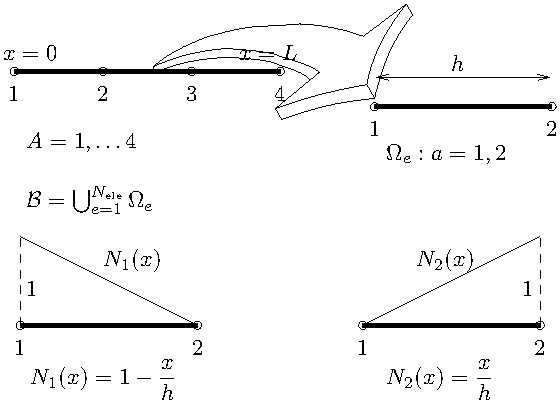
\includegraphics[width=0.6\textwidth]{figuras/func_forma1.pdf}
\caption{Schematic of the linear shape functions of element 2 in the discretisation of a 1D bar with 3 elements.}
\label{fig:funciones_forma}
\end{figure}

Considering the values of $N_1$ y $N_2$ in Fig.~\ref{fig:funciones_forma}, we obtain the integrals to obtain each component of the element stiffness matrix; for example $K_{11}^{e}$ is:
\begin{equation}\label{eq:N9}
K_{11}^{e}=\int_{0}^{h} \frac{\mathrm{d} N_{1}}{\mathrm{d} x} EA \frac{\mathrm{d} N_{1}}{\mathrm{d} x} \mathrm{d} x=\frac{EA}{h^{2}} h=\frac{EA}{h}
\end{equation}

and similarly for the rest of the terms:
\begin{equation}\label{eq:N10}
K_{22}^{e}=\frac{EA}{h} ; \quad K_{12}^{EA}=K_{21}^{e}=-\frac{EA}{h}
\end{equation}
resulting
\begin{equation}\label{eq:N11}
\left[\mathbf{K}^{e}\right]=\frac{EA}{h}\left(\begin{array}{cc}{1} & {-1} \\ {-1} & {1}\end{array}\right)
\end{equation}

Analogously, the volumetric forcing vector is

\begin{equation}\label{eq:N12}
\left\{\mathbf{f}^{\mathrm{vol}, e}\right\}=\frac{h}{6}\left\{\begin{array}{l}{2q_1+q_2} \\ {q_1 + 2q_2}\end{array}\right\}
\end{equation}

%Si considerásemos una carga repartida constante, dicho vector de fuerzas elemental se podría expresar como:
%\begin{equation}
%\left\{\mathbf{f}^{\mathrm{int}, e}\right\}=q h\left\{\begin{array}{l}{1 / 2} \\ {1 / 2}\end{array}\right\}
%\end{equation}\label{eq:N12_bis}

After forming the elementary matrix they are expanded to the global system and numbering

\begin{eqnarray}
K_{a b}^{e} & \rightarrow\left[\hat{\mathbf{K}}^{e}\right] \nonumber
 \\
f_{a}^{e} & \rightarrow \lbrace\hat{\mathbf{f}}^{e}\rbrace \nonumber
\end{eqnarray}

and finally these local matrices are assembled in global matrices of the whole structure. In the example of Fig.~\ref{fig:funciones_forma} all the elements are identical and therefore their stiffness matrix is also the same, being their value the one given in Eq.~\eqref{eq:N11}.

In order to perform the assembly, the location of each element needs to be considered. If we observe Fig.~\ref{fig:funciones_forma} we see that elements 1 and 2 share node 2 (global numbering), that is why position $(2,2)$ in the global stiffness matrix will be shared for the local matrices of elements 1 and 2. The shape of the global matrix is:

\begin{equation}
  K^{global} = \left[
  \begin{BMAT}[8pt]{cccc}{cccc}
   K_{11}^{(1)} & K_{12}^{(1)} & 0 & 0\\
   K_{21}^{(1)} & K_{22}^{(1)}  + K_{11}^{(2)} & K_{12}^{(2)} & 0 \\
    0 & K_{21}^{(2)} & K_{22}^{(2)} + K_{11}^{(3)}  & K_{12}^{(3)} \\
    0 & 0 & K_{21}^{(3)} & K_{22}^{(3)}
  \addpath{(0,4,.)rrddlluu}
  \addpath{(1,3,.)rrddlluu}
   \addpath{(2,2,.)rrddlluu}
  \end{BMAT}\right]
\end{equation}

From this assembly we can obtain the global stiffness matrix by consider values in the local stiffness matrices:

$$
[\mathbf{K}]=\frac{EA}{h}\left(\begin{array}{cccc}{1} & {-1} & {0} & {0} \\ {-1} & {1+1} & {-1} & {0} \\ {0} & {-1} & {1+1} & {-1} \\ {0} & {0} & {-1} & {1}\end{array}\right)
$$
The elementary matrices and global volumetric forcing are:
$$\left\{\mathbf{f}^{\mathrm{vol}, e}\right\}=\frac{h}{6}\left\{\begin{array}{l}{2q_1+q_2} \\ {q_1 + 2q_2}\end{array}\right\}
\Rightarrow\left\{\mathrm{f}^{\mathrm{vol}}\right\}=\frac{h}{6}\left\{\begin{array}{c}{2q_1^{(1)}+q_2^{(1)}} \\ {q_1^{(1)} + 2q_2^{(1)} + 2q_1^{(2)}+q_2^{(2)}} \\ {q_1^{(2)} + 2q_2^{(2)} + 2q_1^{(3)}+q_2^{(3)}}  \\ {q_1^{(3)} + 2q_2^{(3)}}\end{array}\right\}
$$

Considering a restriction of the movement at the left end $x=0$ and a point load $q_L$ applied at the right end $x=L$, the matricial equation that results from the FE method is:
$$[\mathbf{K}]\{\mathbf{u}\}=\left\{\mathbf{f}^{\text {vol }}\right\}+\left\{\mathbf{f}^{\text {ext }}\right\}
$$
\begin{equation}\label{sistema}
\frac{EA}{h}\left(\begin{array}{c;{2pt/2pt}ccc}{1} & {-1} & {0} & {0} \\ 
\hdashline[2pt/2pt]
{-1} & {1+1} & {-1} & {0} \\ {0} & {-1} & {1+1} & {-1} \\ {0} & {0} & {-1} & {1}\end{array}\right)
\left\{\begin{array}{l}0\\
\hdashline[2pt/2pt]
u_2 \\ u_{3} \\ u_{4}\end{array}
\right\}=
\frac{h}{6}\left\{\begin{array}{c}{2q_1^{(1)}+q_2^{(1)}} \\ 
\hdashline[2pt/2pt]
{q_1^{(1)} + 2q_2^{(1)} + 2q_1^{(2)}+q_2^{(2)}} \\ {q_1^{(2)} + 2q_2^{(2)} + 2q_1^{(3)}+q_2^{(3)}}  \\ {q_1^{(3)} + 2q_2^{(3)}}\end{array}\right\}
+\left\{\begin{array}{c} R_0 \\
\hdashline[2pt/2pt]
{0} \\ {0} \\ {P}\end{array}\right\}
\end{equation}

\clearpage
 
The volumetric forcing vector is added to the vector representing the external actions, which in this case it is a load in $P$. On the other hand, at the left end $x=0$ there is a reaction given by imposing the displacement in this point, $u(0)=0$. Such reaction is obtained \textit{afterwards}, once the nodal displacements are obtained $\{\mathbf{u}\}$. \\
 
 The global stiffness matrix is reduced to remove the degrees of freedom associated with the boundary conditions of the problem. This is followed by the calculation of the nodal displacements solving the algebraic system of equations through the inversion of the reduced global stiffness matrix. After this is done, equilibrium can be checked from the sum of the internal forces in the structure:

$$
\left\{\mathbf{f}^{\text {int}}\right\}=[\mathbf{K}]\{\mathbf{u}\}
$$

which should be 0.
 
 On the other hand, the reaction in this case could be obtained by multiplying the eliminated row in the global stiffness matrix $[\mathbf{K}]$ (corresponding to the boundary condition of imposed displacement) times the vector of displacements and subtracting the forces applied at the that node (which can only be volumetric forces because the boundary condition of type Dirichlet):
 $$
 R_0=K_{1j}u_j-f^{\text {vol}}_1
$$

\paragraph{Important observation.---}
You will see that in this structural problem, which is extremely simple, the FE solution in terms of displacements and stresses is exactly the same as the exact analytical value at the nodes of the numerical model. This is called \emph{``superconvergent'' problem} and it happens because the only error introduced in the FE model is observed at the intermediate sections between nodes, i.e. within the finite elements, being exact the values at the nodes and at the integration points.

This is not generally the case in other, more complicated, problems in which the solution at the nodes diverges from the exact value at those points.



\clearpage

\section{FE simulation with Abaqus}
\label{sec:abaqus}

We will analyse the response of a 1D elastic bar with length \(L=10 \mathrm{mm}\) and constant section \(A=1 \mathrm{mm}^{2} .\) The material of the bar is linear elastic, with a Young Modulus \(E=1000 \mathrm{MPa}\).
The left end \((x=0)\) is fully fixed and the right end \((x=L)\) has an applied point axial load \(P=5 \mathrm{N},\) as shown in Fig.~\ref{fig:esq}. It is assumed that deformations are small.

\begin{figure}[!htp]
\centering
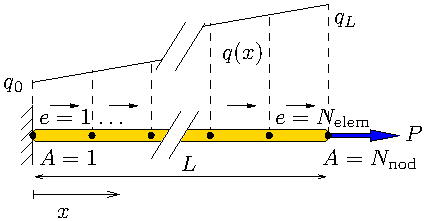
\includegraphics[width=0.7\textwidth]{figuras/esquema.pdf}
\caption{Elastic 1D bar model}
\label{fig:esq}
\end{figure}

Using the hundreds (c), tens (d) and units ( \(u\) ) of your student number the parameters defining the model will be obtained as:

\begin{itemize}
\item Number of elements for the FE discretisation of the bar \(N_{\text {elem }}=11-c\)
\item The distributed load \(q(x),\) per unit length in the along-bar direction will vary linearly from the two ends of the bar \(x=0\) y \(x=L,\) with the following values at both ends \(q_0=d / 10\; \mathrm{N} / \mathrm{mm}, \quad q_{L}=q_{0}+u / 10 \; \mathrm{N} / \mathrm{mm} \), respectively.
\end{itemize}

The FE code of the problem should follow these steps:
% Note from Alfredo Camara, why this part is here if it deals with programming? It seems that the current section is on the use of ABAQUS.

\begin{enumerate}
\item Propose the elastic problem and boundary conditions.
\item Calculate the numerical expressions of the global stiffness matrix and forcing vectors.
\item Application of boundary conditions and solution of the algebraic system of equations.
\item Solution of the displacements \(u(x)\) and stresses \(\sigma(x)\) at each point. Plot the graphs in terms of the along-bar coordinate \(x\) and compare the results with the analytical solution. (Note: the stresses are obtained from the nodal displacements as \(\sigma=E \varepsilon=E \mathrm{d} u / \mathrm{d} x,\) and using the internal displacement interpolation of each finite element, \(\left.\sigma^{h}=E u_{a} \mathrm{d} N_{a} / \mathrm{d} x=E\left(u_{2}-u_{1}\right) / h .\right)\)
\end{enumerate}

We will start using the commercial FE software \texttt{Abaqus} to obtain the results of the proposed problem.
Even though it is a 1D problem we will model the bar with 3D elements to help visualising the structure following similar steps to those in the first practical session, but now doing our first 3D model.

\subsection{The \texttt{Part} module}


First we will create a new model in \emph{Abaqus CAE}. Go to the \texttt{part} module, click in the icon to create a new part and select 3D deformable, extrusion solid (figure \ref{fig:bar1a}). We will create a rectangle (figur \ref{fig:bar1b}) from the corner points with coordinates (-0.5,-0.5) and (0.5,0.5) in mm. Therefore the area will be 1 mm$^2$ as intended.
\begin{figure}[h!tp]
\centering
\captionsetup[subfigure]{justification=centering,singlelinecheck=false}
  \begin{subfigure}[b]{0.38\textwidth}
  \hspace{10mm}
    \imagebox{90mm}{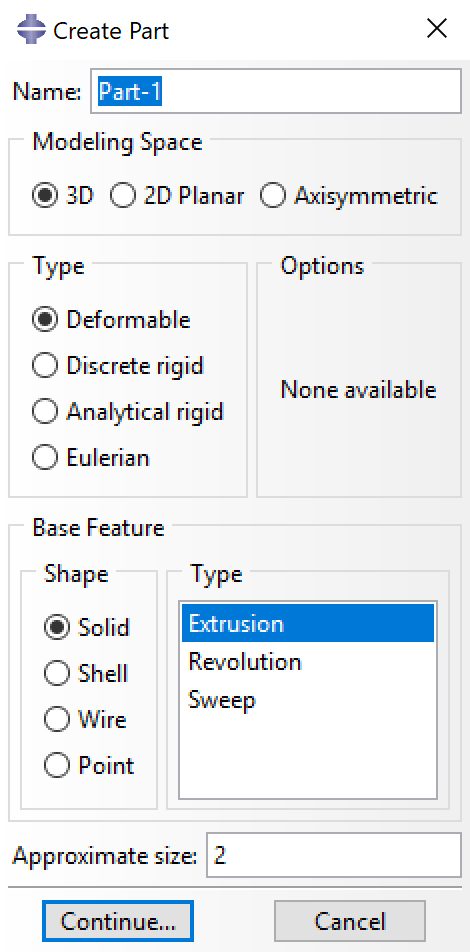
\includegraphics[scale=0.51]{capturas/solid.png}}
    \caption{Part/solid\label{fig:bar1a}}
  \end{subfigure}
  \begin{subfigure}[b]{0.25\textwidth}
  \hspace{6mm}
    \imagebox{90mm}{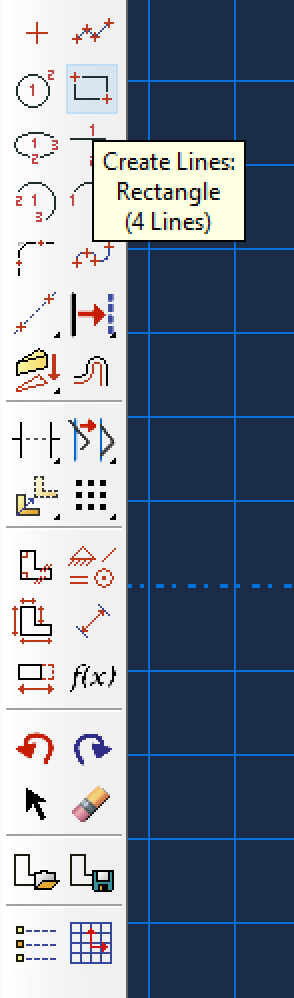
\includegraphics[scale=0.5]{capturas/rectangulo.png}}
    \caption{Rectangle\label{fig:bar1b}}
  \end{subfigure}
\caption{Definition of the geometry.}
\label{fig:bar1}
\end{figure}

After this is done we click in \emph{done} (or press the wheel of your mouse if you have it) and define the length of the bar in direction \emph{Z}, which in our case is 10 mm. You should see a body similar to that in Fig. \ref{fig:bar2b}.

\begin{figure}[h!tp]
\centering
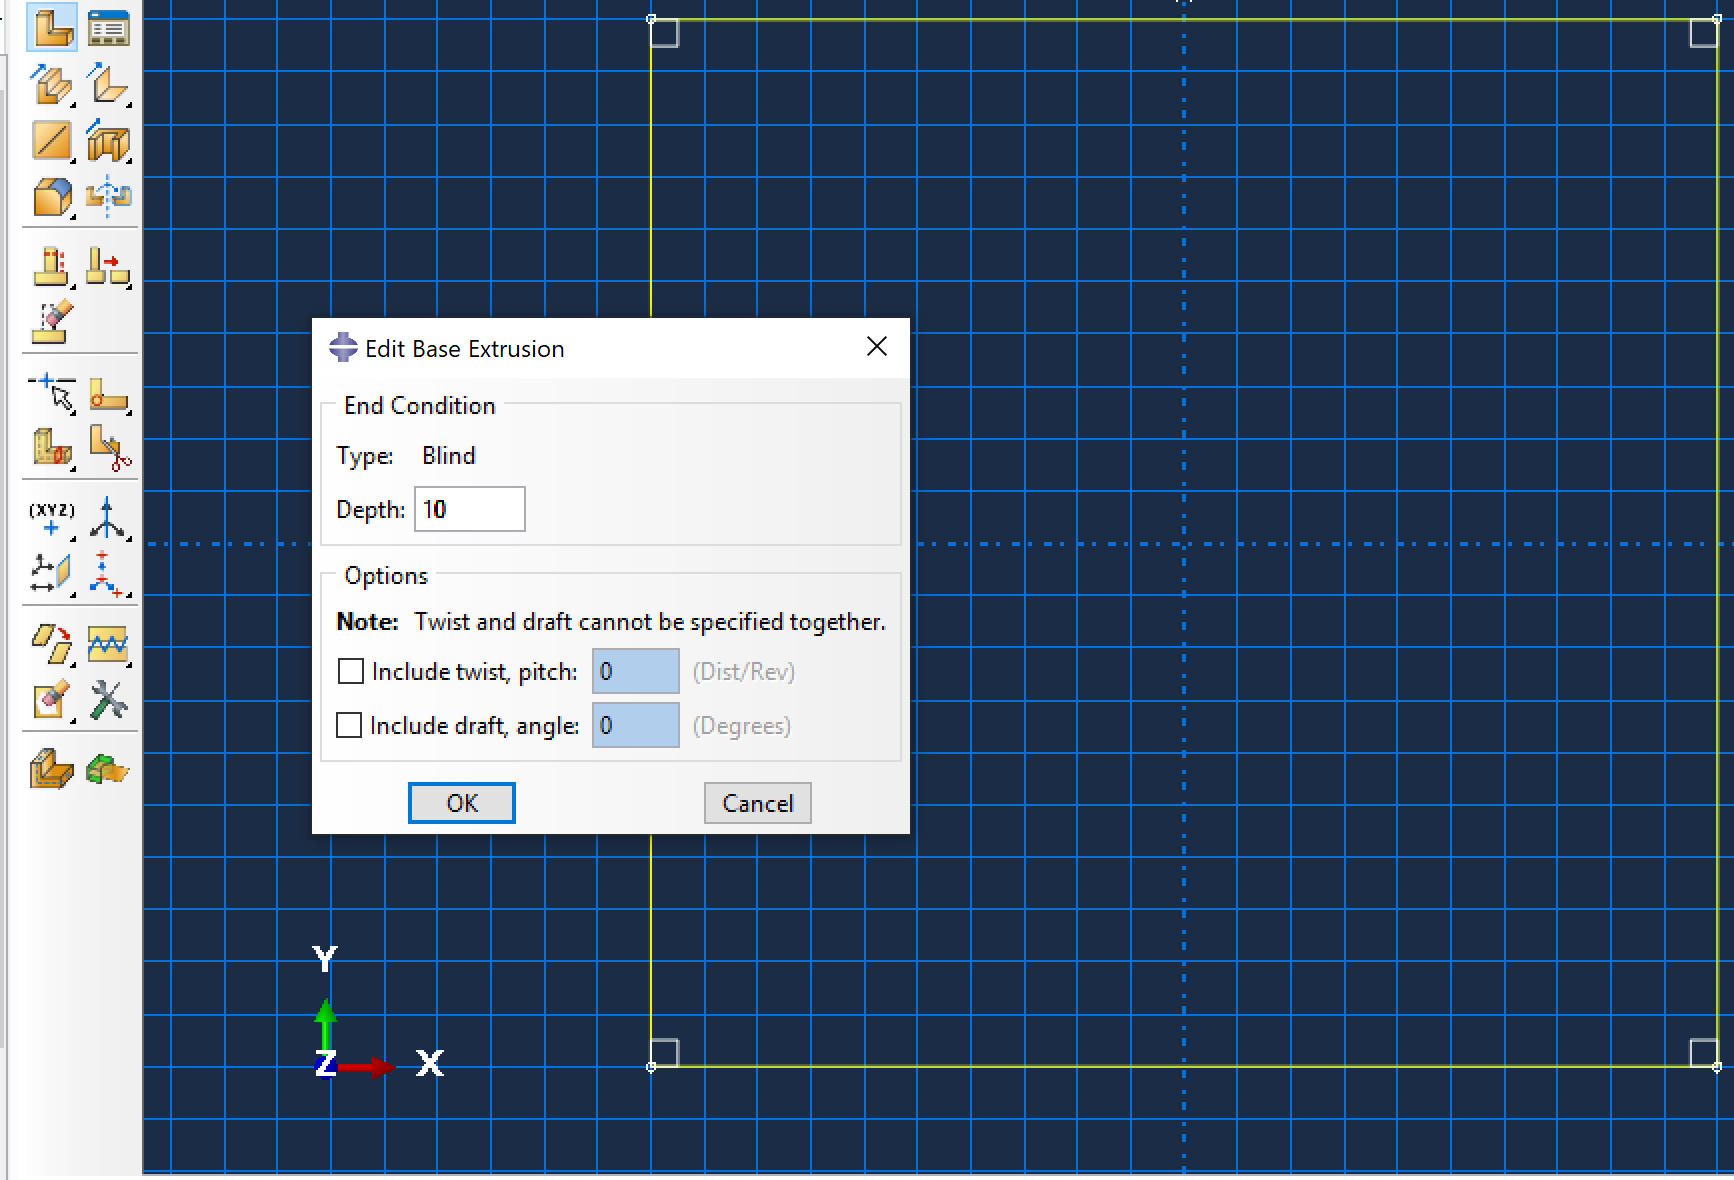
\includegraphics[scale=0.4]{capturas/sec1.png}
\caption{Extrussion of the section.}
\label{fig:bar2a}
\end{figure}
\begin{figure}[h!tp]
\centering
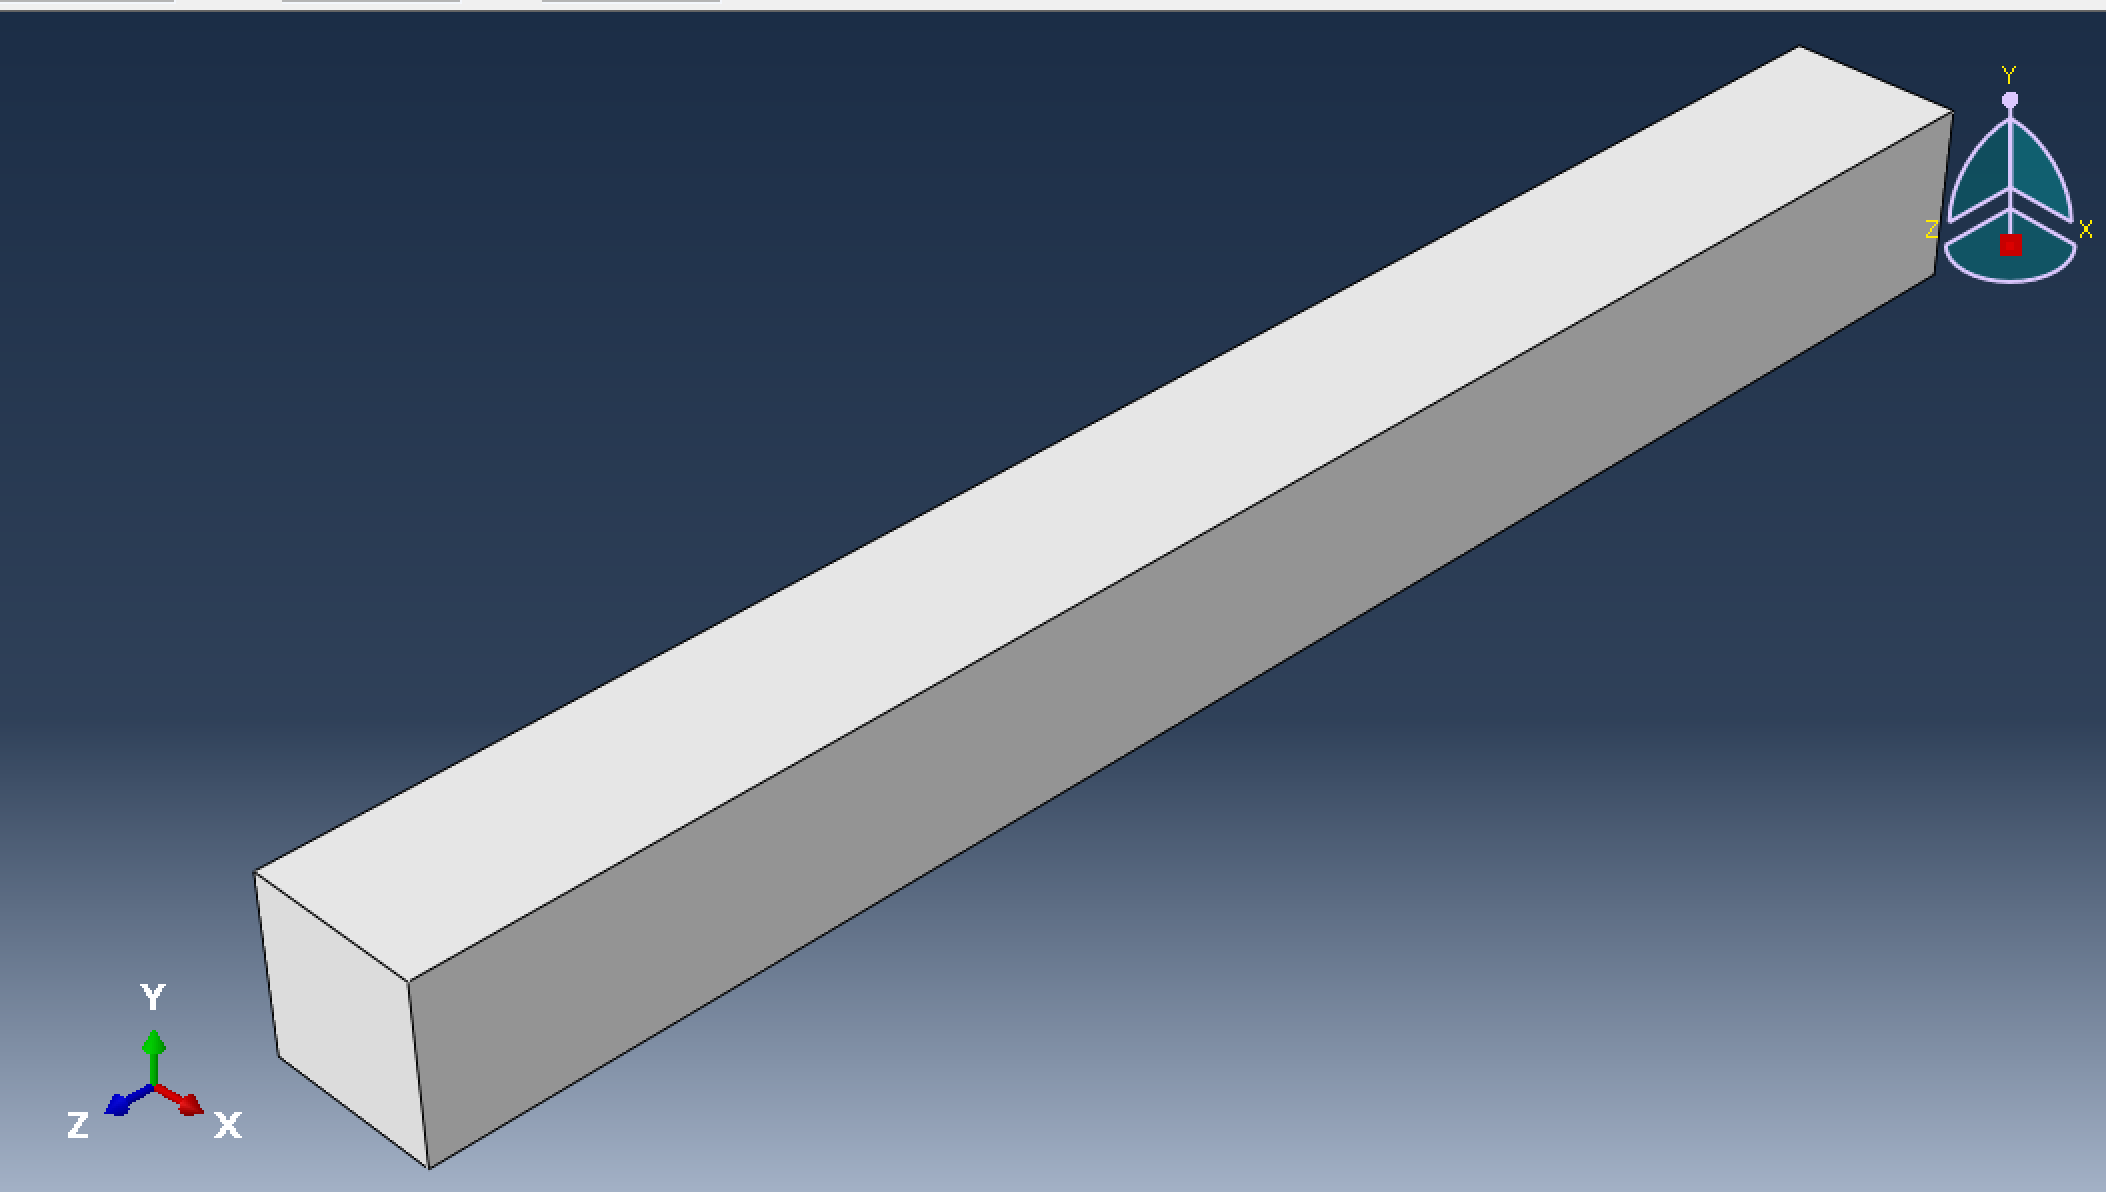
\includegraphics[scale=0.30]{capturas/sec2.png}
\caption{Final geometry of the bar.}
\label{fig:bar2b}
\end{figure}


\subsection{The \texttt{Property} module}

Create a new material (figure \ref{fig:bar3}) and select elastic linear material with the properties $E=1000\,\text{MPa}, \nu=0$. Remember the dimensional relationships defined in the first practical session; we defined the geometry in mm and therefore we need to use MPa=N/mm$^2$ for the stress and the Young's modulus. 

Create a \emph{``section''} of type \emph{solid}-homogeneous (figure \ref{fig:bar4a}) and chose the material previously created.

Assign the newly created section to the bar (figura \ref{fig:bar4b}) by selecting the whole volume. Confirm by clicking the icon \emph{Done}.
\begin{figure}[h!tp]
\centering
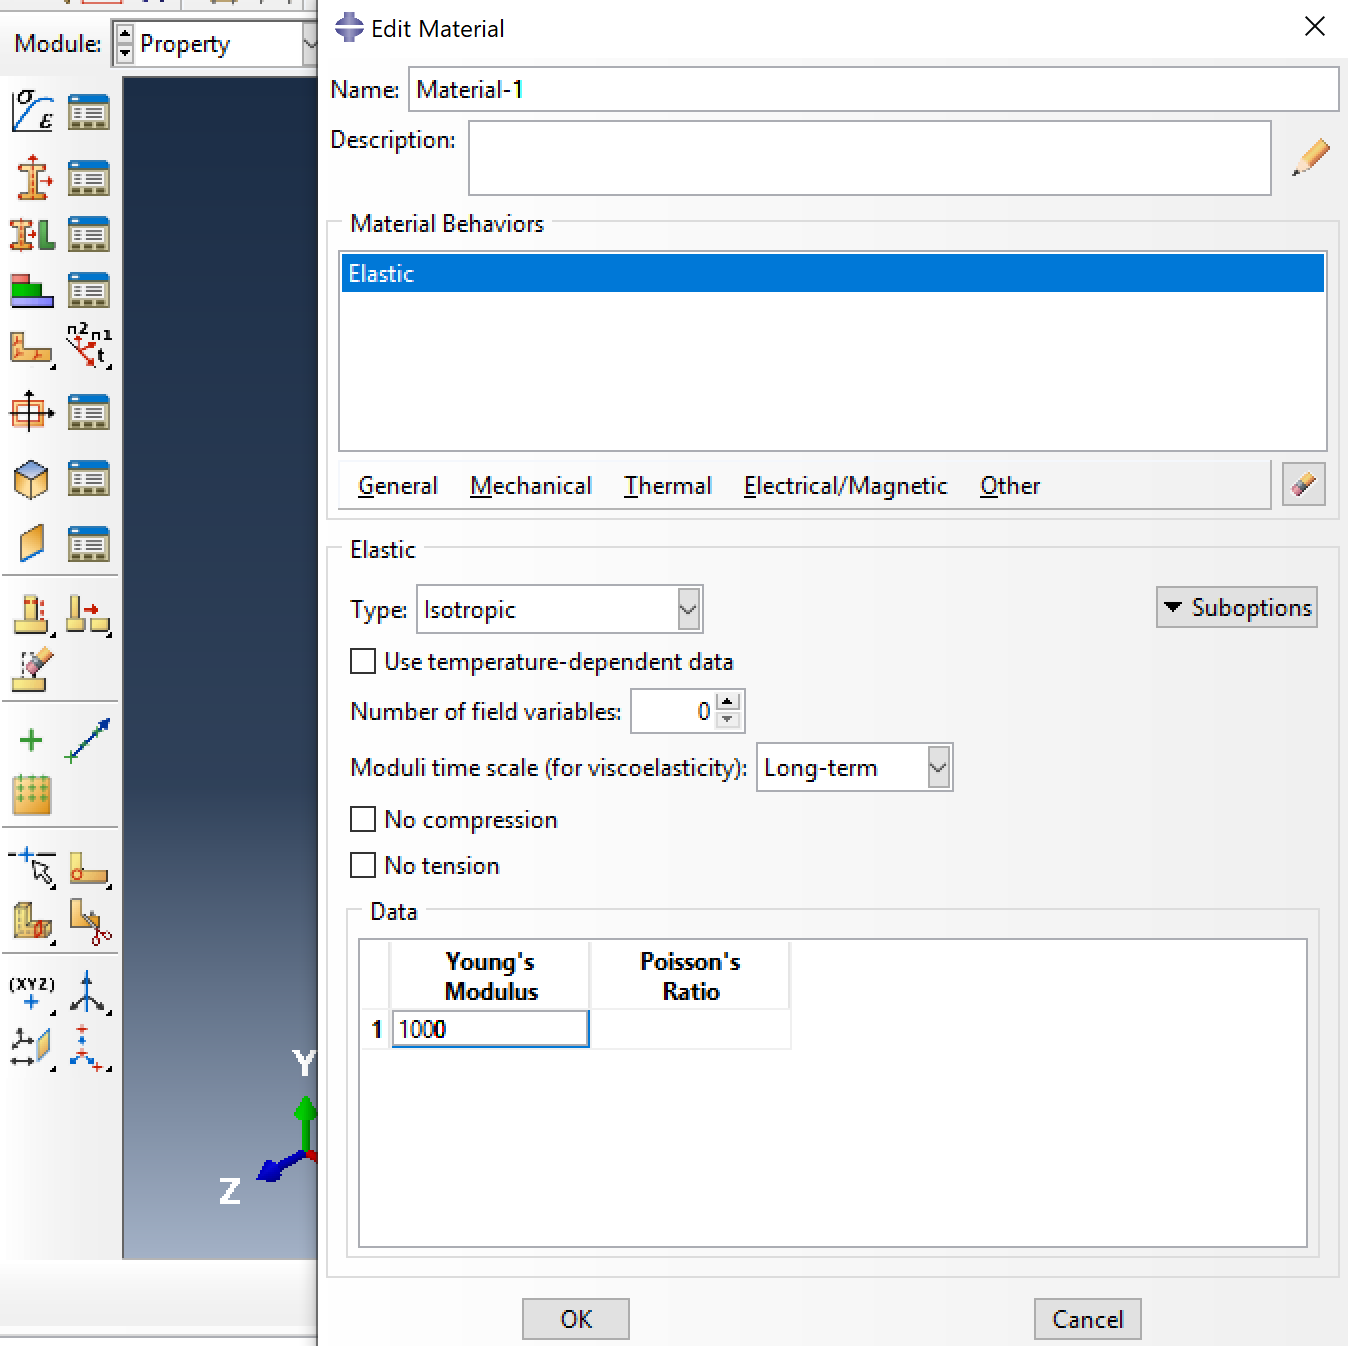
\includegraphics[scale=0.4]{capturas/prop0.png}
\caption{Elastic material.}
\label{fig:bar3}
\end{figure}

\begin{figure}[h!tp]
\centering
\captionsetup[subfigure]{justification=centering,singlelinecheck=false}
  \begin{subfigure}[b]{0.20\textwidth}
  \hspace{0mm}
    \imagebox{75mm}{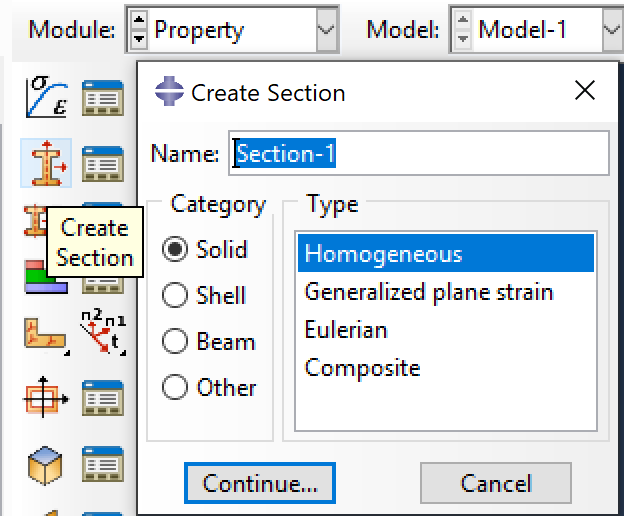
\includegraphics[scale=0.3]{capturas/prop1.png}}
    \caption{Create section\label{fig:bar4a}}
  \end{subfigure}
  \begin{subfigure}[b]{0.79\textwidth}
  \hspace{0mm}
    \imagebox{75mm}{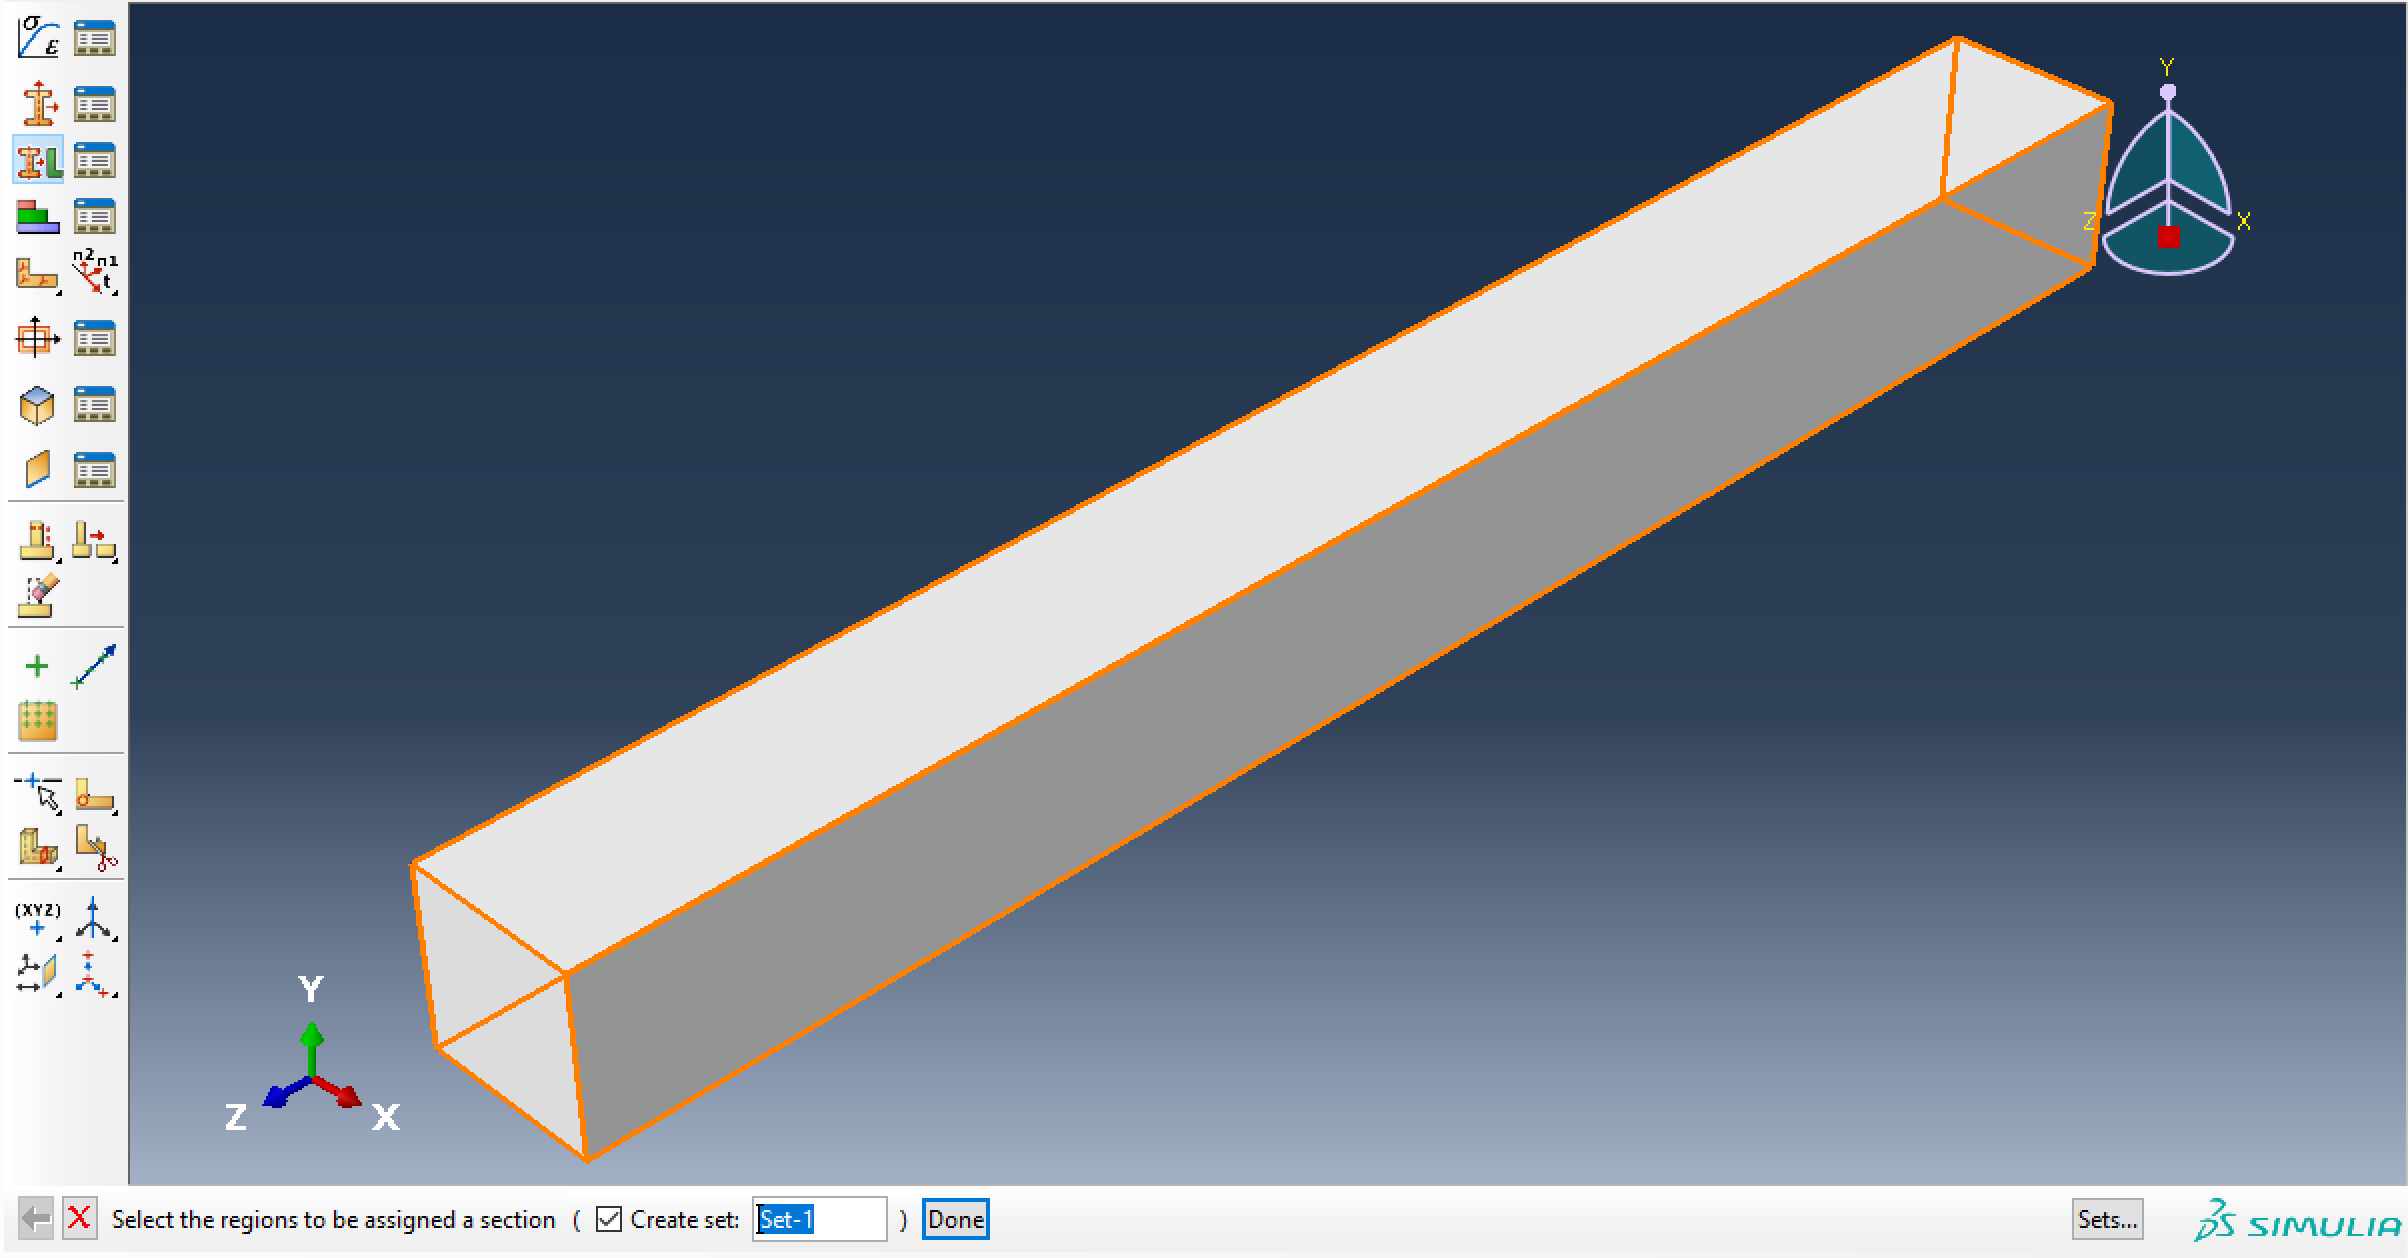
\includegraphics[scale=0.32]{capturas/prop2.png}}
    \caption{Assign section\label{fig:bar4b}}
  \end{subfigure}
\caption{How to select the section}
\label{fig:bar4}
\end{figure}

\clearpage
\subsection{The \texttt{Assembly} module}

In this module you only need to create an ``Instance'' from the part previously defined. This can be done by means of the default options shown in Fig. \ref{fig:assembly}.


\begin{figure}[h!tp]
\centering
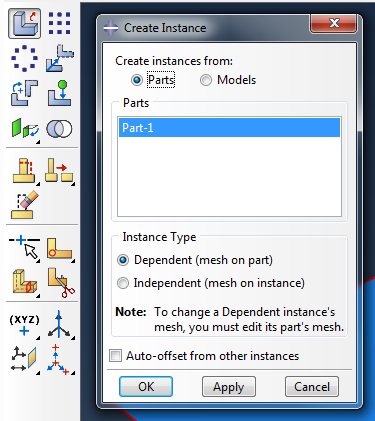
\includegraphics[scale=0.4]{capturas/14-assembly.png}
\caption{Assembly: create an instance from the part.}
\label{fig:assembly}
\end{figure}

\subsection{The \texttt{Step} module}

Create an analysis ``step'' that is ``Static, general'' using the default options (figure \ref{fig:step}). 
It is not necessary to edit the requested ``field output'' because it includes the default response variables that we will need in our study.

\begin{figure}[h!tp]
\centering
\captionsetup[subfigure]{justification=centering,singlelinecheck=false}
  \begin{subfigure}[b]{0.35\textwidth}
  \hspace{10mm}
    \imagebox{90mm}{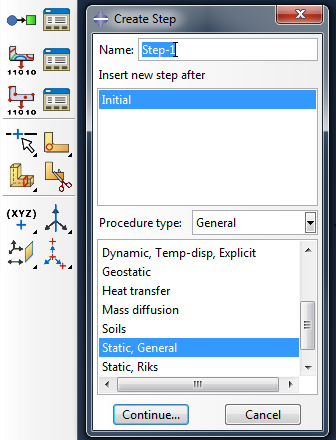
\includegraphics[scale=0.4]{capturas/15-step.png}}
  \end{subfigure}
  \begin{subfigure}[b]{0.64\textwidth}
  \hspace{6mm}
    \imagebox{90mm}{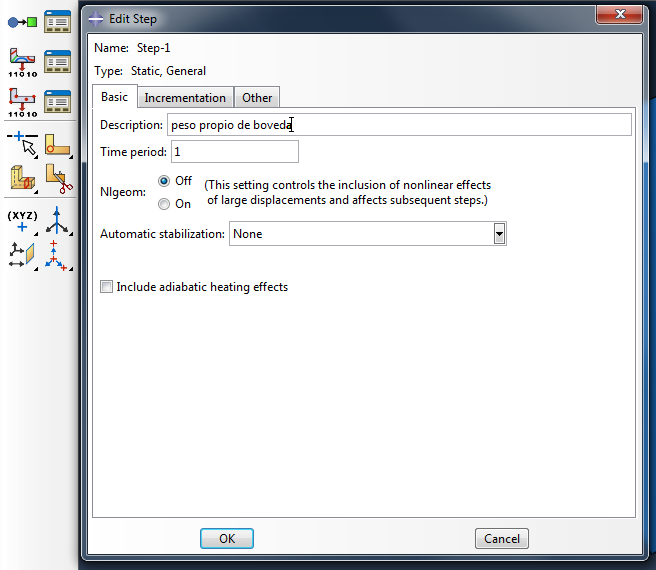
\includegraphics[scale=0.4]{capturas/16-step.png}}
  \end{subfigure}
\caption{Create and define the analysis ``step''.}
\label{fig:step}
\end{figure}

\clearpage
\subsection{The \texttt{Load} module}
We must define in this module the two types of boundary conditions. First, at the left end \emph{Z=0} we clamp the bar. To this end we create a \emph{Boundary Condition}that is \emph{Mechanical} (category) and the type is \emph{Encastre} (figure \ref{fig:load1}).

\begin{figure}[h!tp]
\centering
\captionsetup[subfigure]{justification=centering,singlelinecheck=false}
  \begin{subfigure}[b]{0.4\textwidth}
  \hspace{0mm}
    \imagebox{60mm}{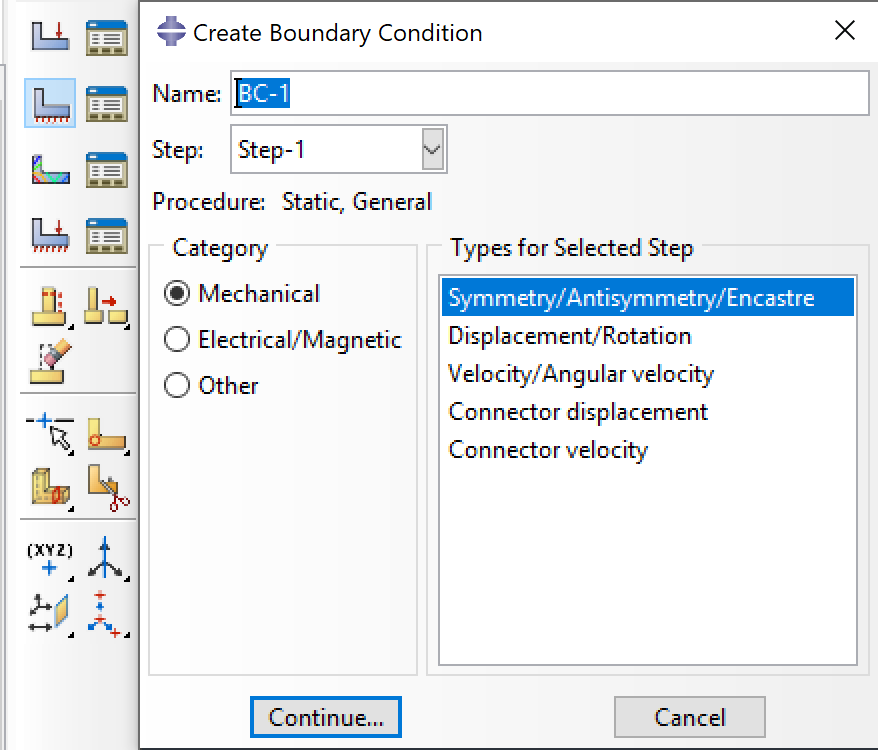
\includegraphics[scale=0.4]{capturas/load1.png}}
  \end{subfigure}
  \begin{subfigure}[b]{0.59\textwidth}
  \hspace{1mm}
    \imagebox{60mm}{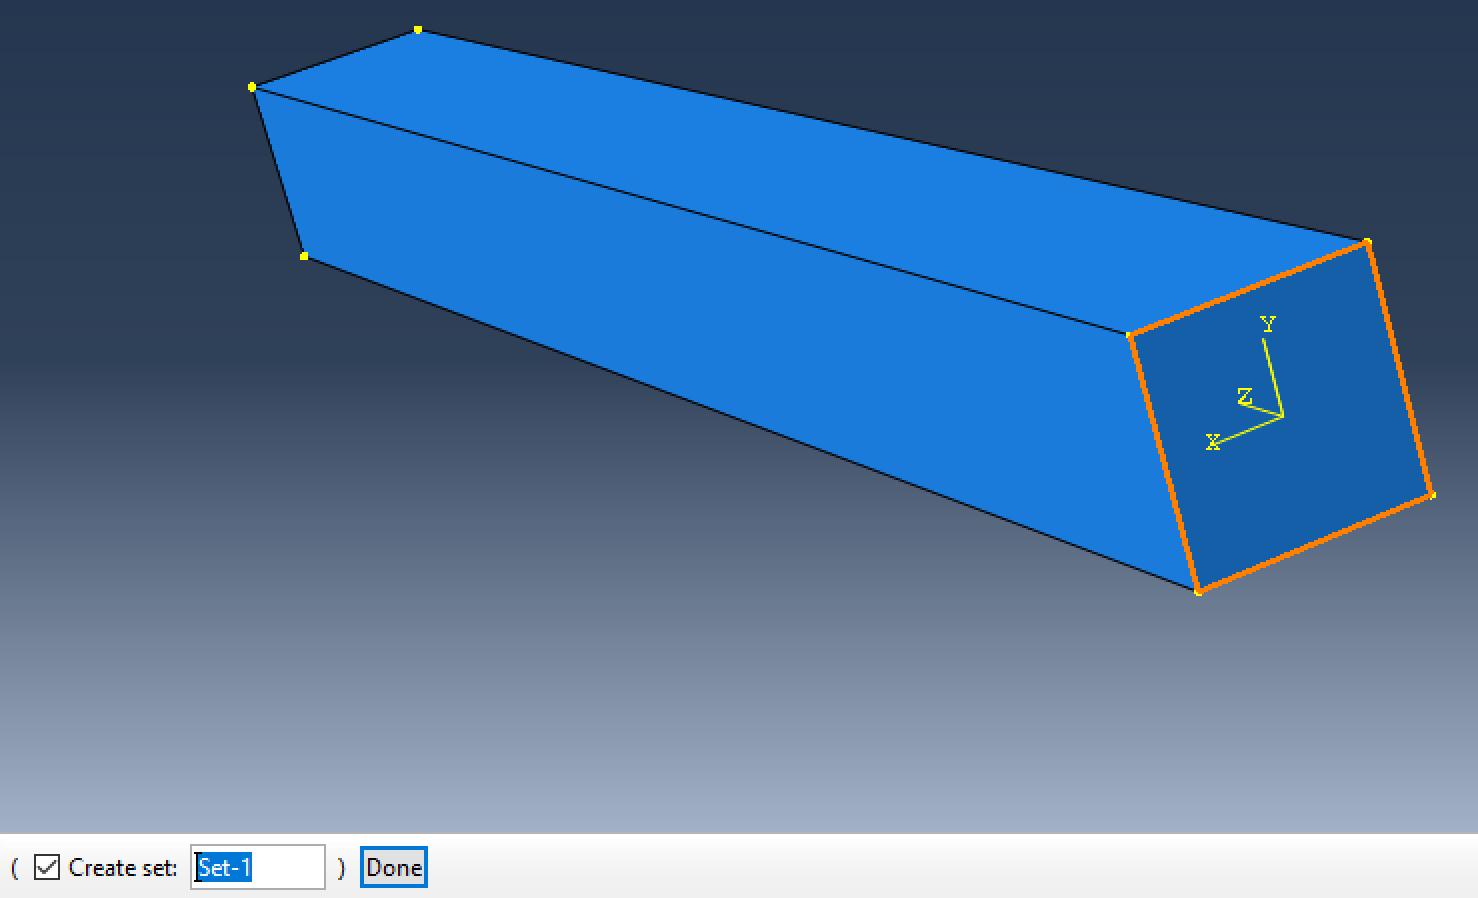
\includegraphics[scale=0.35]{capturas/load2.png}}
  \end{subfigure}
\caption{Creation of the encastre conditions}
\label{fig:load1}
\end{figure}

Once the surface to clamp (encastre) is defined and then confirmed clicking \emph{Done}, we must select the type of condition to assign to this region of the bar. To this end we select \emph{Encastre} from the possible options (figure \ref{fig:load2}.

\begin{figure}[h!tp]
\centering
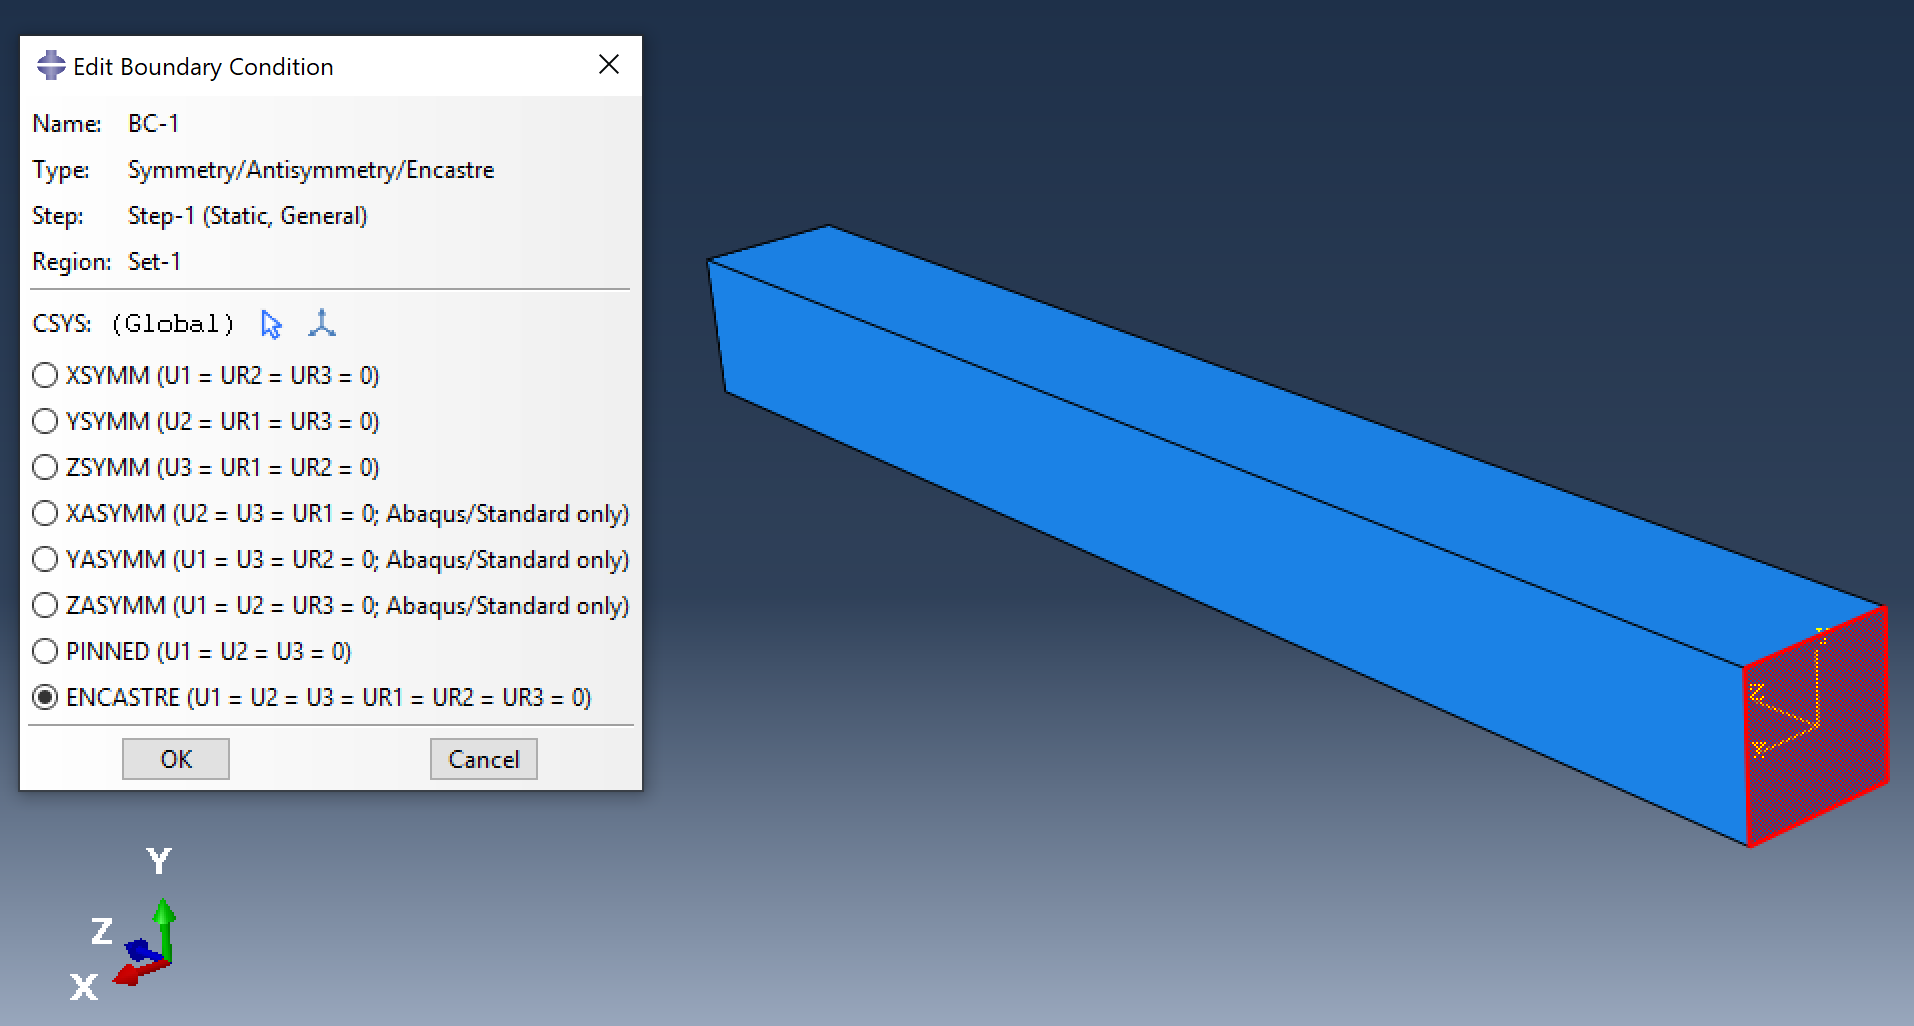
\includegraphics[scale=0.4]{capturas/load3.png}
\caption{Defition of \emph{Boundary Condition: Encastre}.}
\label{fig:load2}
\end{figure}

Now we define the two loads in our our problem: a point load and a volumetric load. With respect to the point load it can be defined in different ways. The easiest one to apply a traction at the surface \emph{Z=L}, which is a load of category \emph{Mechanical} and type \emph{Surface Traction} in \texttt{Abaqus} (figure \ref{fig:load3a}). Next, we select the surface where the traction is going to be applied and the window with the options to define the load will be displayed (figura \ref{fig:load3b}). The load is uniformly distributed, and the traction is of type  \emph{General} (i.e. it is not a shear force but a normal action). In order to define the direction of the load we need to define the normal to the surface, which in this case is a vector parallel to the positive  \emph{Z} axis, therefore we can define it as a unit vector (0,0,1). The magnitude of the traction will be $5 N$ (force) divided over the surface area where it is applied, 1 mm$^2$, thus the applied pressure is, 5 MPa.

\clearpage
\begin{figure}[h!tp]
\centering
\captionsetup[subfigure]{justification=centering,singlelinecheck=false}
  \begin{subfigure}[b]{0.74\textwidth}
  \hspace{0mm}
    \imagebox{75mm}{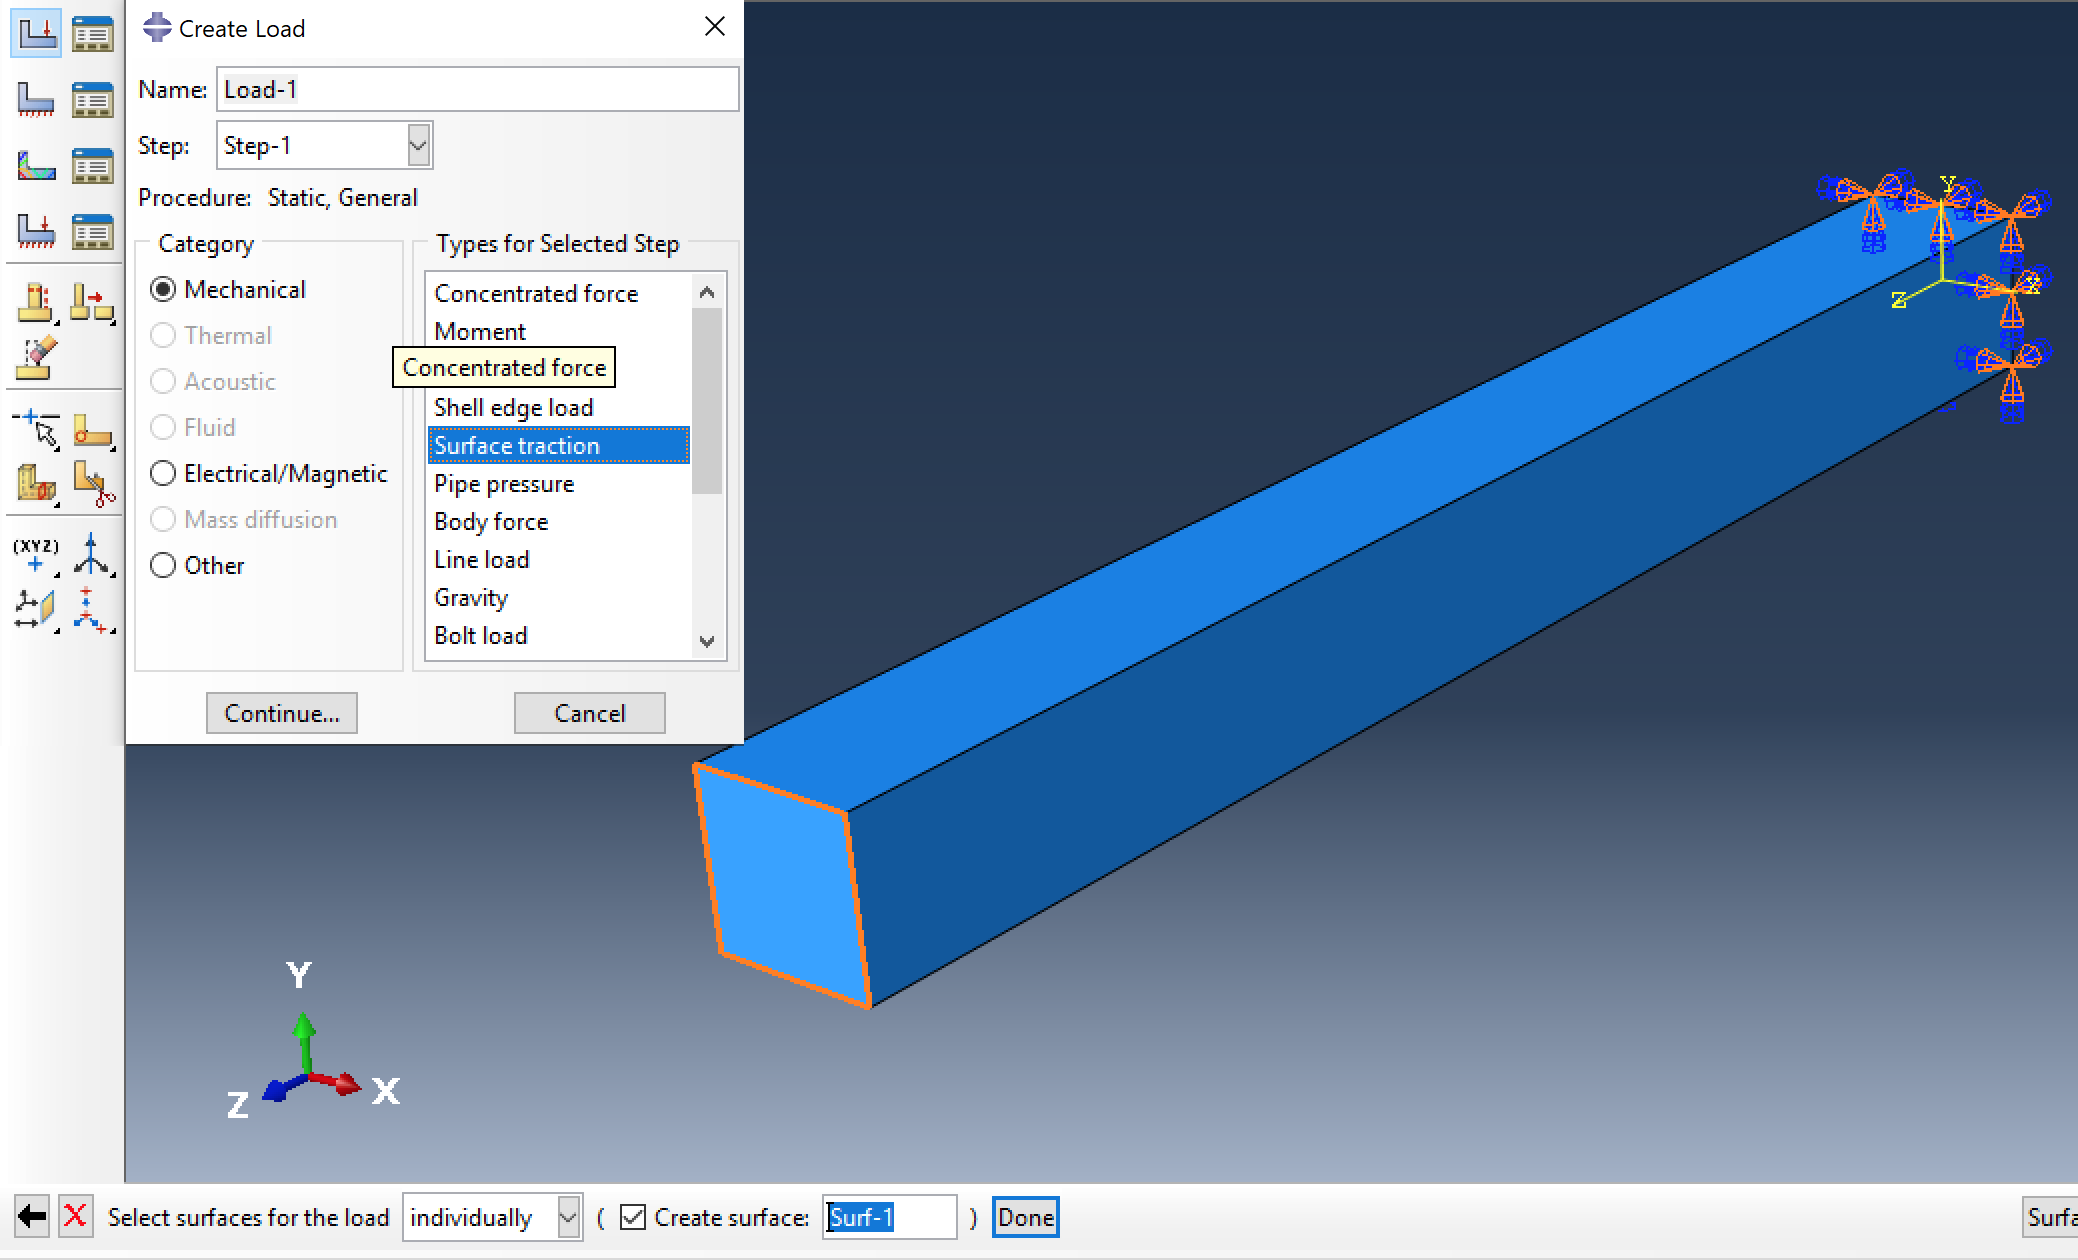
\includegraphics[scale=0.32]{capturas/load4.png}}
    \caption{Definition of the load surface\label{fig:load3a}}
  \end{subfigure}
  \begin{subfigure}[b]{0.25\textwidth}
  \hspace{0mm}
    \imagebox{75mm}{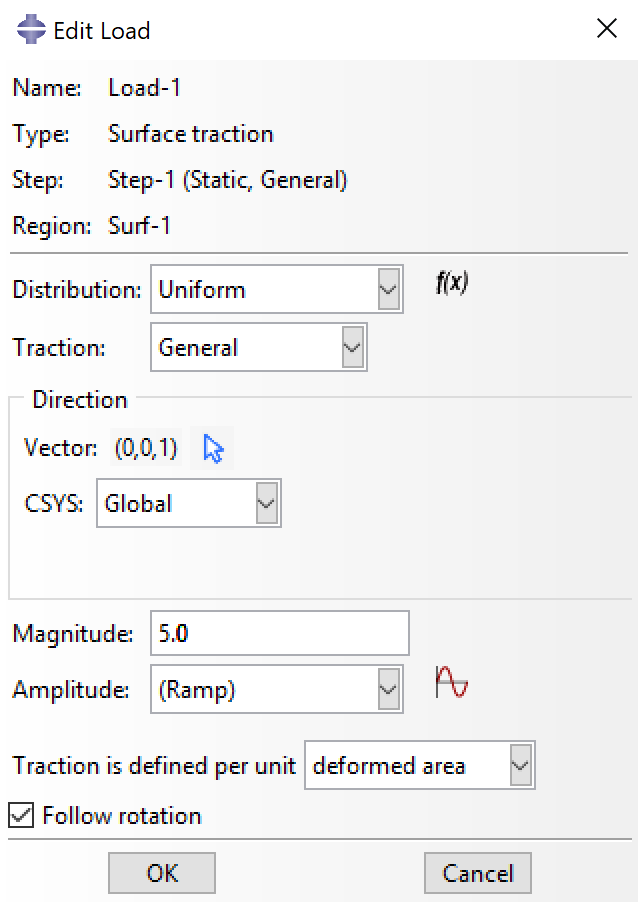
\includegraphics[scale=0.46]{capturas/load5.png}}
    \caption{Definition of the load direction and magnitude\label{fig:load3b}}
  \end{subfigure}
\caption{Definition of the load at the end of the bar.}
\label{fig:load3}
\end{figure}

With respect to the volumetric force, it has to be defined in the entire volume of the bar. First you need to select \emph{Body Force} as the forcing type when creating the load. Afterwards, this load has to be assigned to the entire structure (figure \ref{fig:load4}). Then we need to define the magnitude of the load. To this end we click in the icon with a symbol $f(x)$ because it will not be uniform but a function of the coordinates, in this case $Z$. This expression is defined in the window \emph{Expression Field} the pops out when hitting $f(x)$. Considering that the student's registration number (número de  matrícula) for the development of this exercise is 1024, the expression is $q=0.2 + 0.04*Z$. This is what we need to introduce in the corresponding box. Once the expression is created, in the field \emph{Distribution} of the window \emph{Edit Load} we assign the newly generated \emph{Expression Field} which in our case is \emph{AnalyticalField-1}. The component will be (0,0,0), that is, direction \emph{Z}.

% ACC: it is not clear that (0,0,0) point at Z.

\begin{figure}[h!tp]
\centering
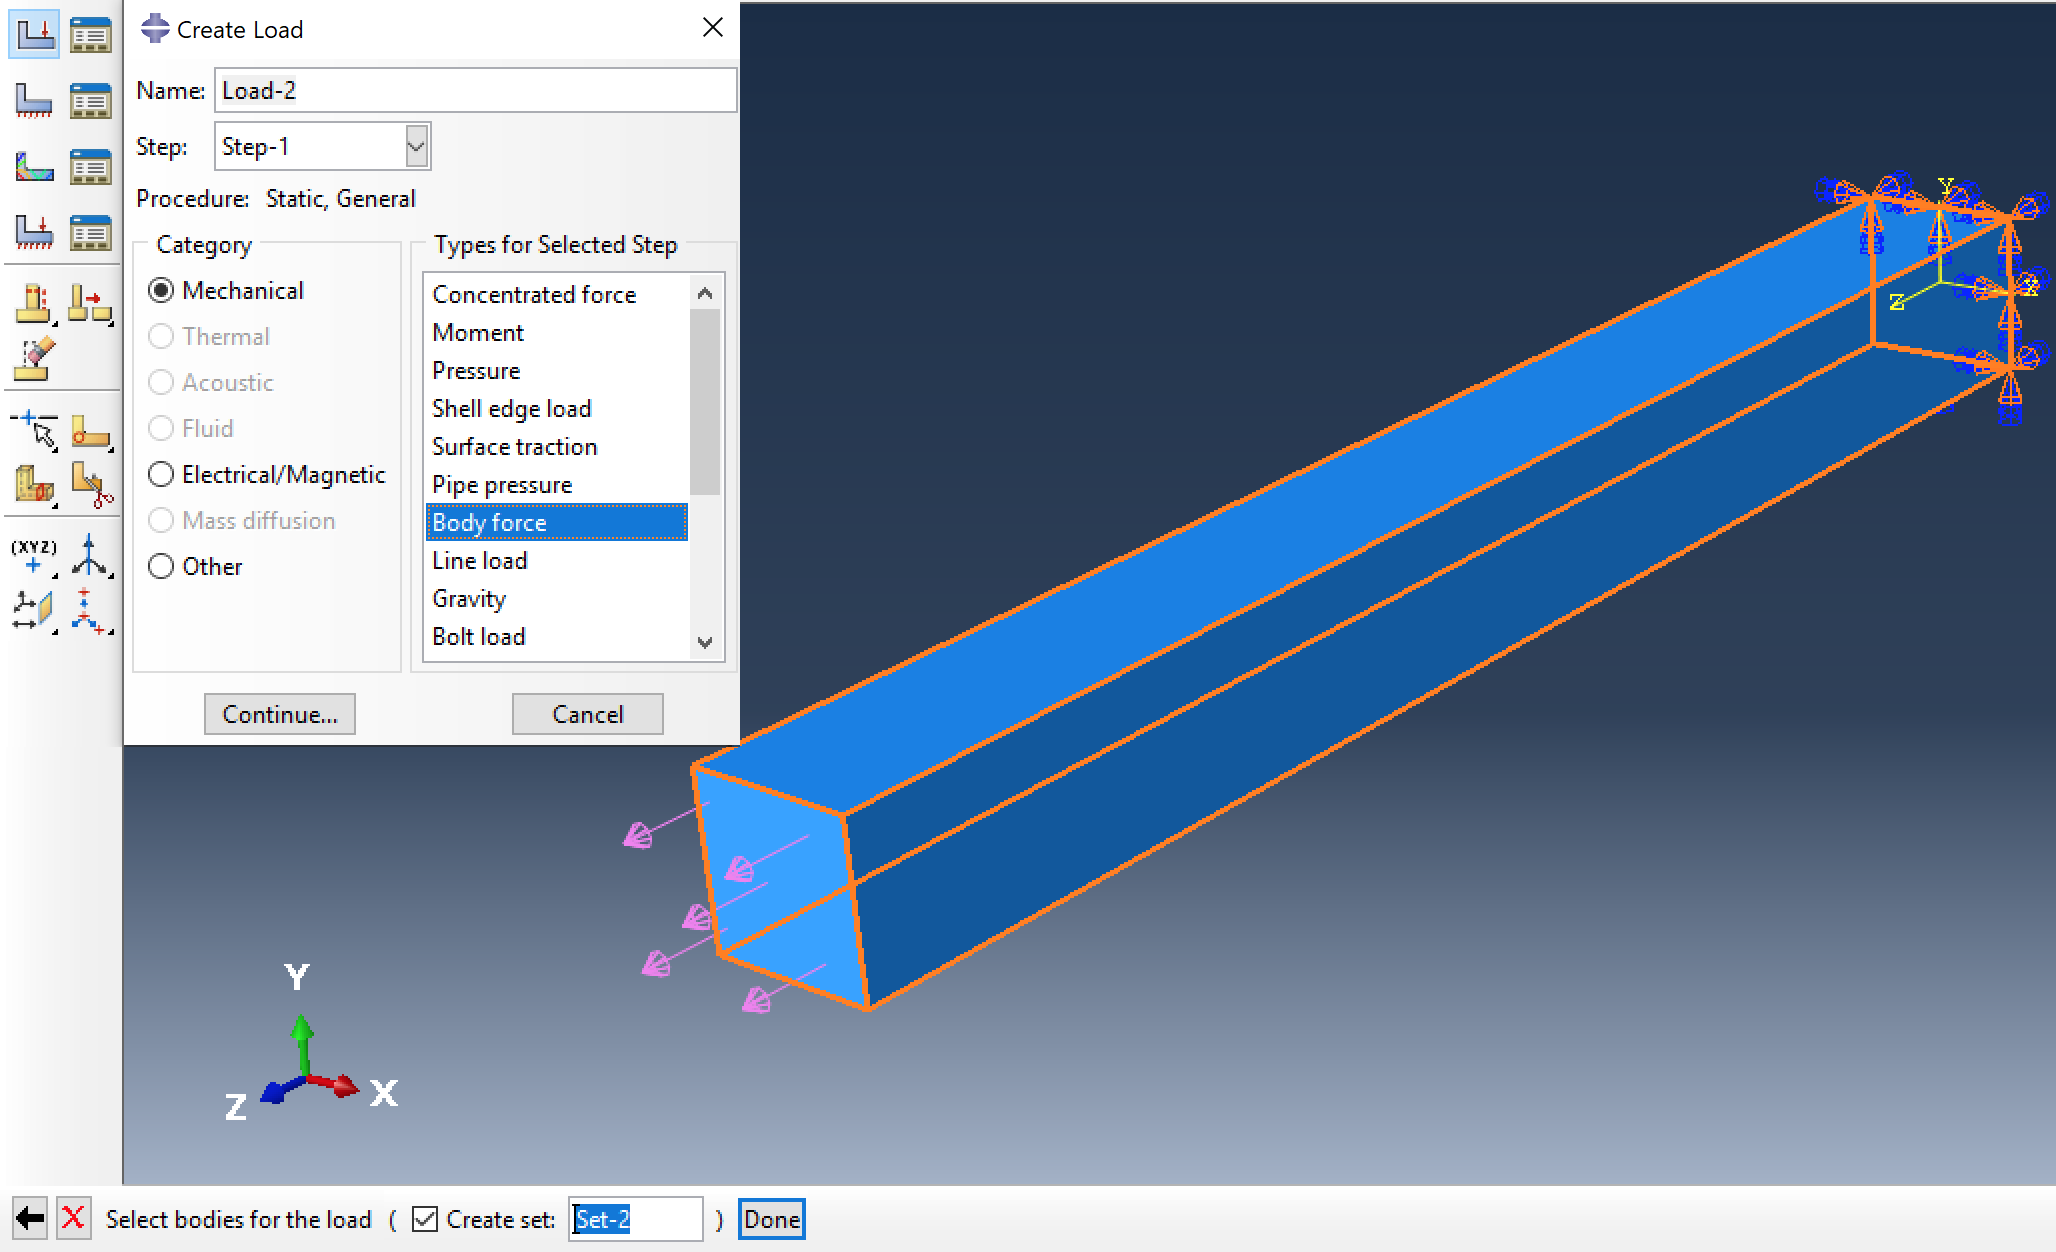
\includegraphics[scale=0.35]{capturas/load6.png}
\caption{Creation of the \emph{Body Force}}
\label{fig:load4}
\end{figure}


\clearpage
\begin{figure}[h!tp]
\centering
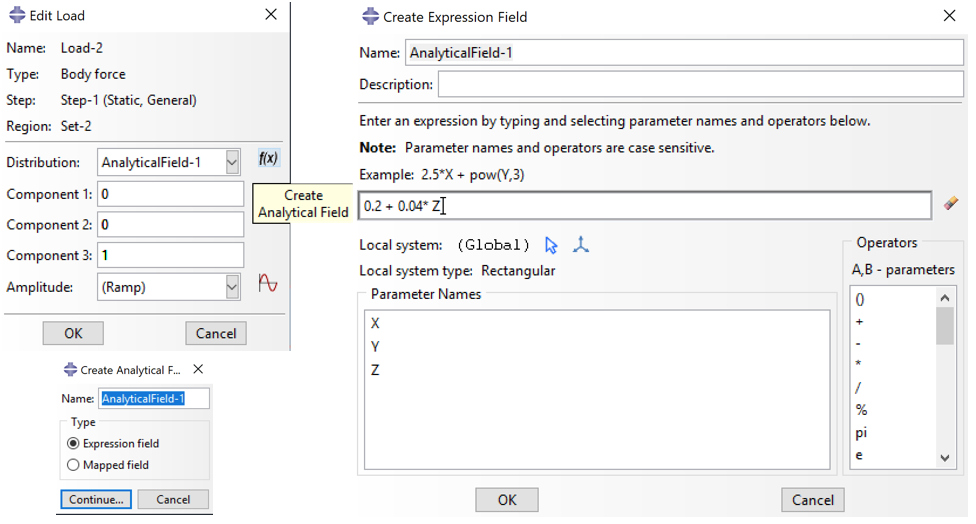
\includegraphics[scale=0.85]{capturas/load7.png}
\caption{Definition of the load distribution with an \emph{Expression Field}}
\label{fig:load5}
\end{figure}

Once the second load is defined the model should look like the one in Fig. \ref{fig:load6}.

\begin{figure}[h!tp]
\centering
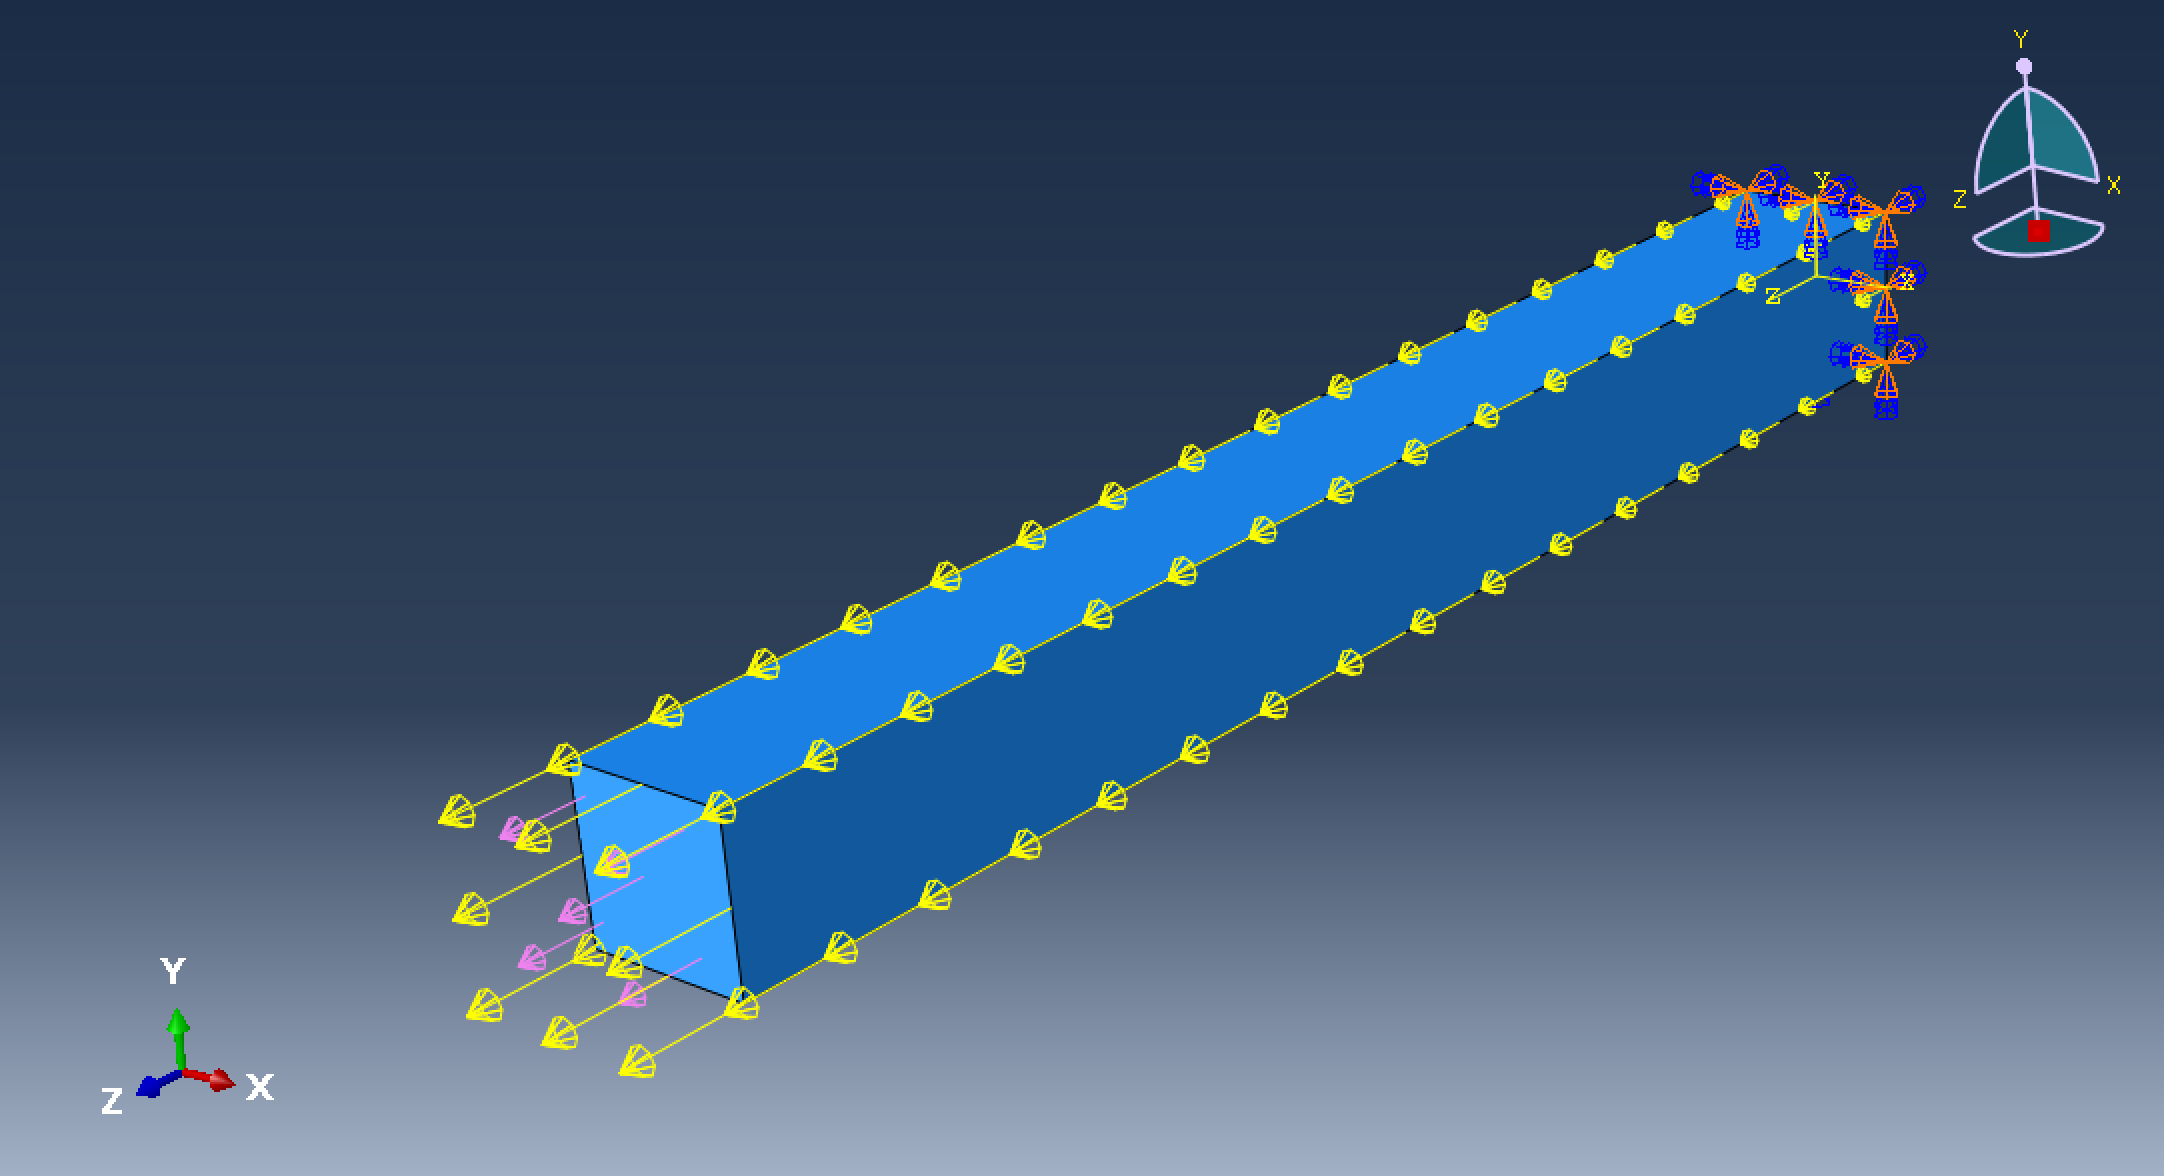
\includegraphics[scale=0.38]{capturas/load8.png}
\caption{Complete set of loads}
\label{fig:load6}
\end{figure}

\clearpage

\subsection{The \texttt{Mesh} module}

In the Mesh module we define the finite element discretisation. We start by selecting the Part, expanding the model tree on the left side of the screen, and activating with a right click of your mouse in the icon \emph{``Mesh''}:
Fig.~\ref{fig:mesh-part}.
%Open in the top menu bar \emph{Mesh} $\to$ \emph{Controls} and select ``Hex'' and ``Structured'', to generate s structured mesh of quadrilaterals 

% ACC changed quadrilaterals by hexahedra below

This will open the \emph{Mesh} menu. Go to \emph{Controls} and select ``Hex'' and ``Structured'' to generate an structured mesh of regular hexahedra
(Fig. \ref{fig:mesh-controls}).
\begin{figure}[h!tp]
\parbox[t]{0.49\textwidth}{%
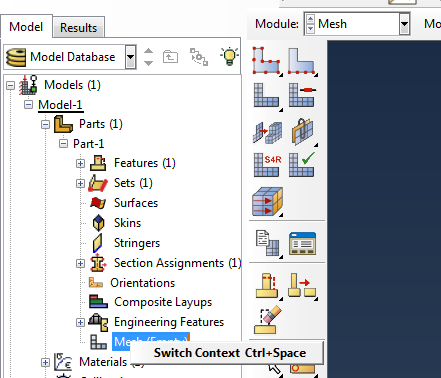
\includegraphics[width=0.5\textwidth]{capturas/29-mesh.png}
%\caption{Expanded model tree for mesh.}
\caption{Select the menu to mesh.}
\label{fig:mesh-part}%
}\quad
\parbox[t]{0.49\textwidth}{%
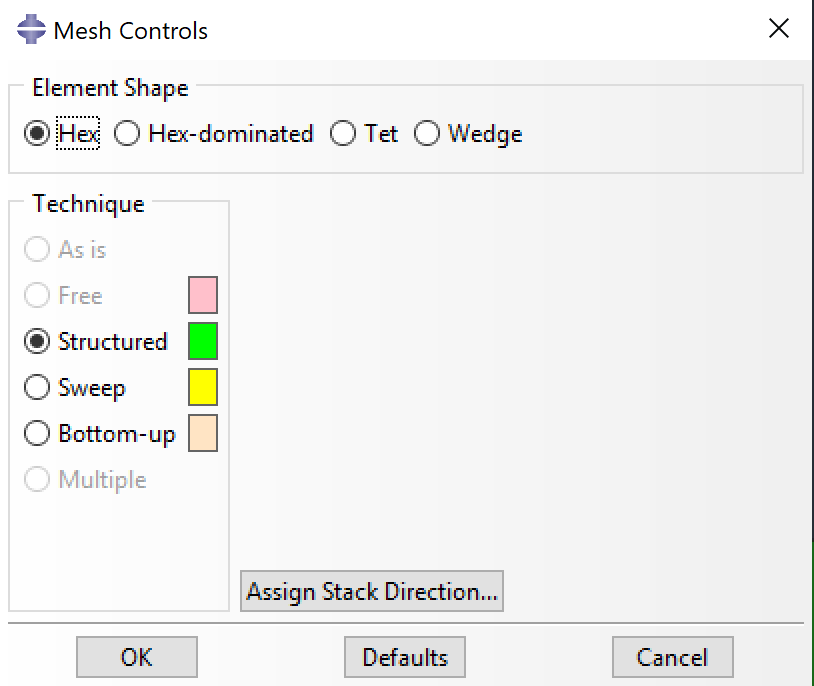
\includegraphics[width=0.5\textwidth]{capturas/30-mesh-x.png}
%\caption{Define options in ``Mesh controls''}
\caption{Define options in ``Mesh controls''}
\label{fig:mesh-controls}%
}%
\end{figure}

%Following, open in the top bar the menu \emph{Mesh} $\to$ \emph{Element type} and select the options \emph{``3D stress''}, \emph{``Membrane stress: Linear''}, \emph{``Reduced integration''} which will correspond to element type C3D8R, enough for the involved calculation

The following step is to open the menu \emph{Mesh} $\to$ \emph{Element type} and select the options ``3D Stress'', ``Linear'', \emph{``Reduced integration''}. This will select the element type C3D8R in \emph{Abaqus}, which is sufficient for the analysis that we will perform. 
(Fig. \ref{fig:mesh-element}).
\begin{figure}[h!tp]
\centering
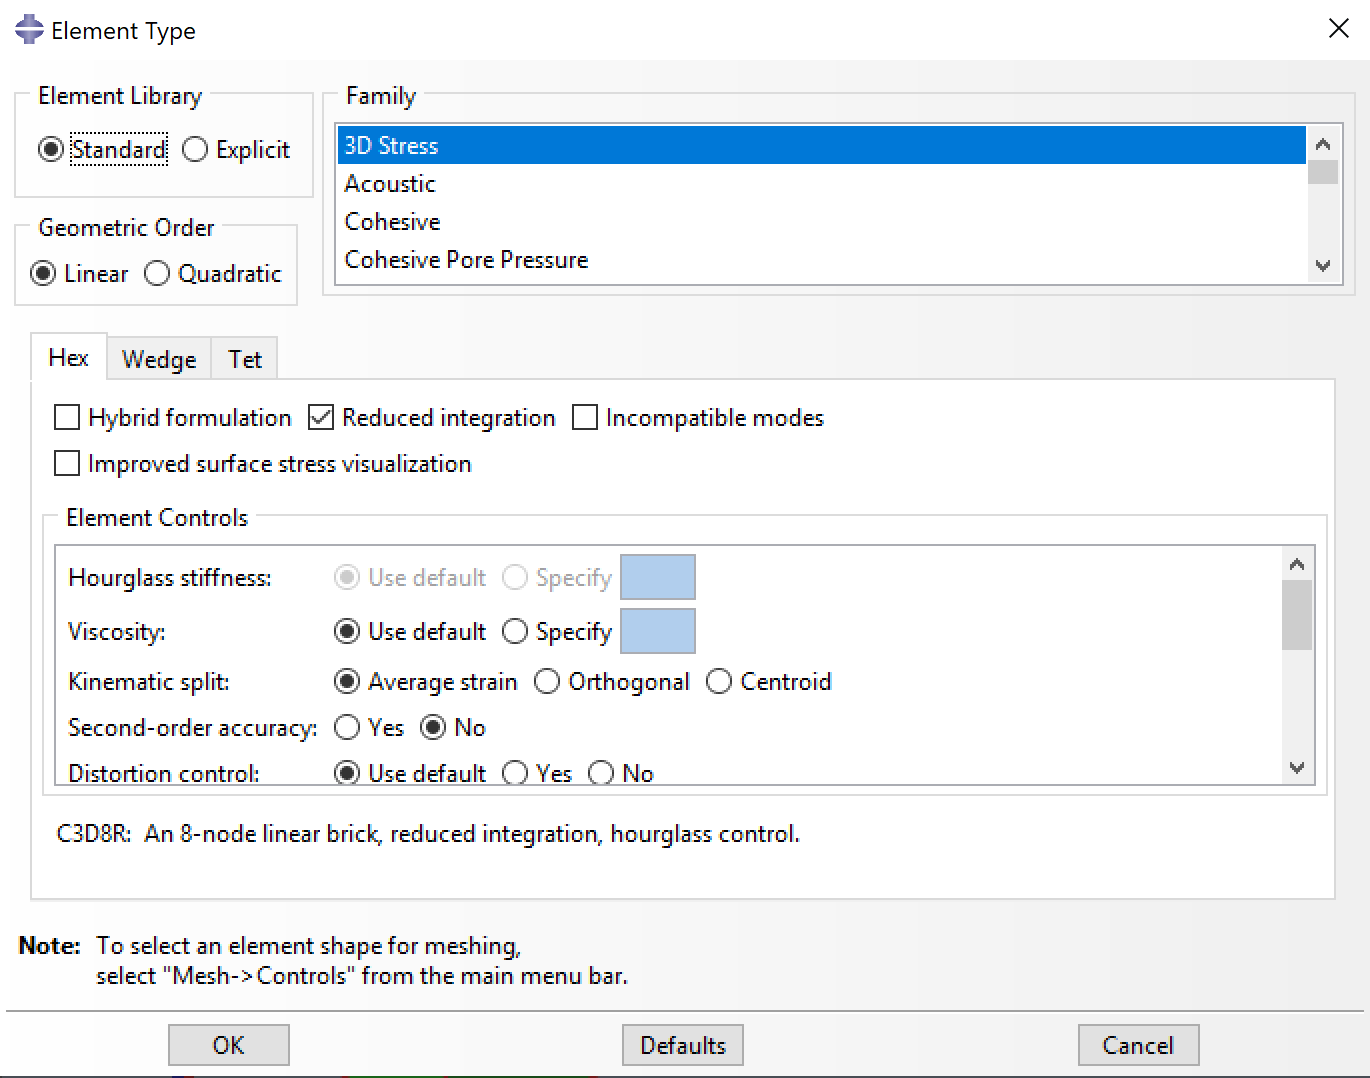
\includegraphics[scale=0.4]{capturas/31-mesh.png}
\caption{Select the element type in ``Mesh/element''}
\label{fig:mesh-element}%
\end{figure}

You need to select the  \emph{``Seed''} of the mesh, which is the approximate size of the elements in your model. We chose 1 mm as the size of elements in all the space direction, which will lead to 10 hexahedral elements in the longitudinal direction of the bar (Fig. \ref{fig:mesh1}). This will result in the mesh shown in Fig. \ref{fig:mesh1}.

\clearpage
\begin{figure}[h!tp]
\centering
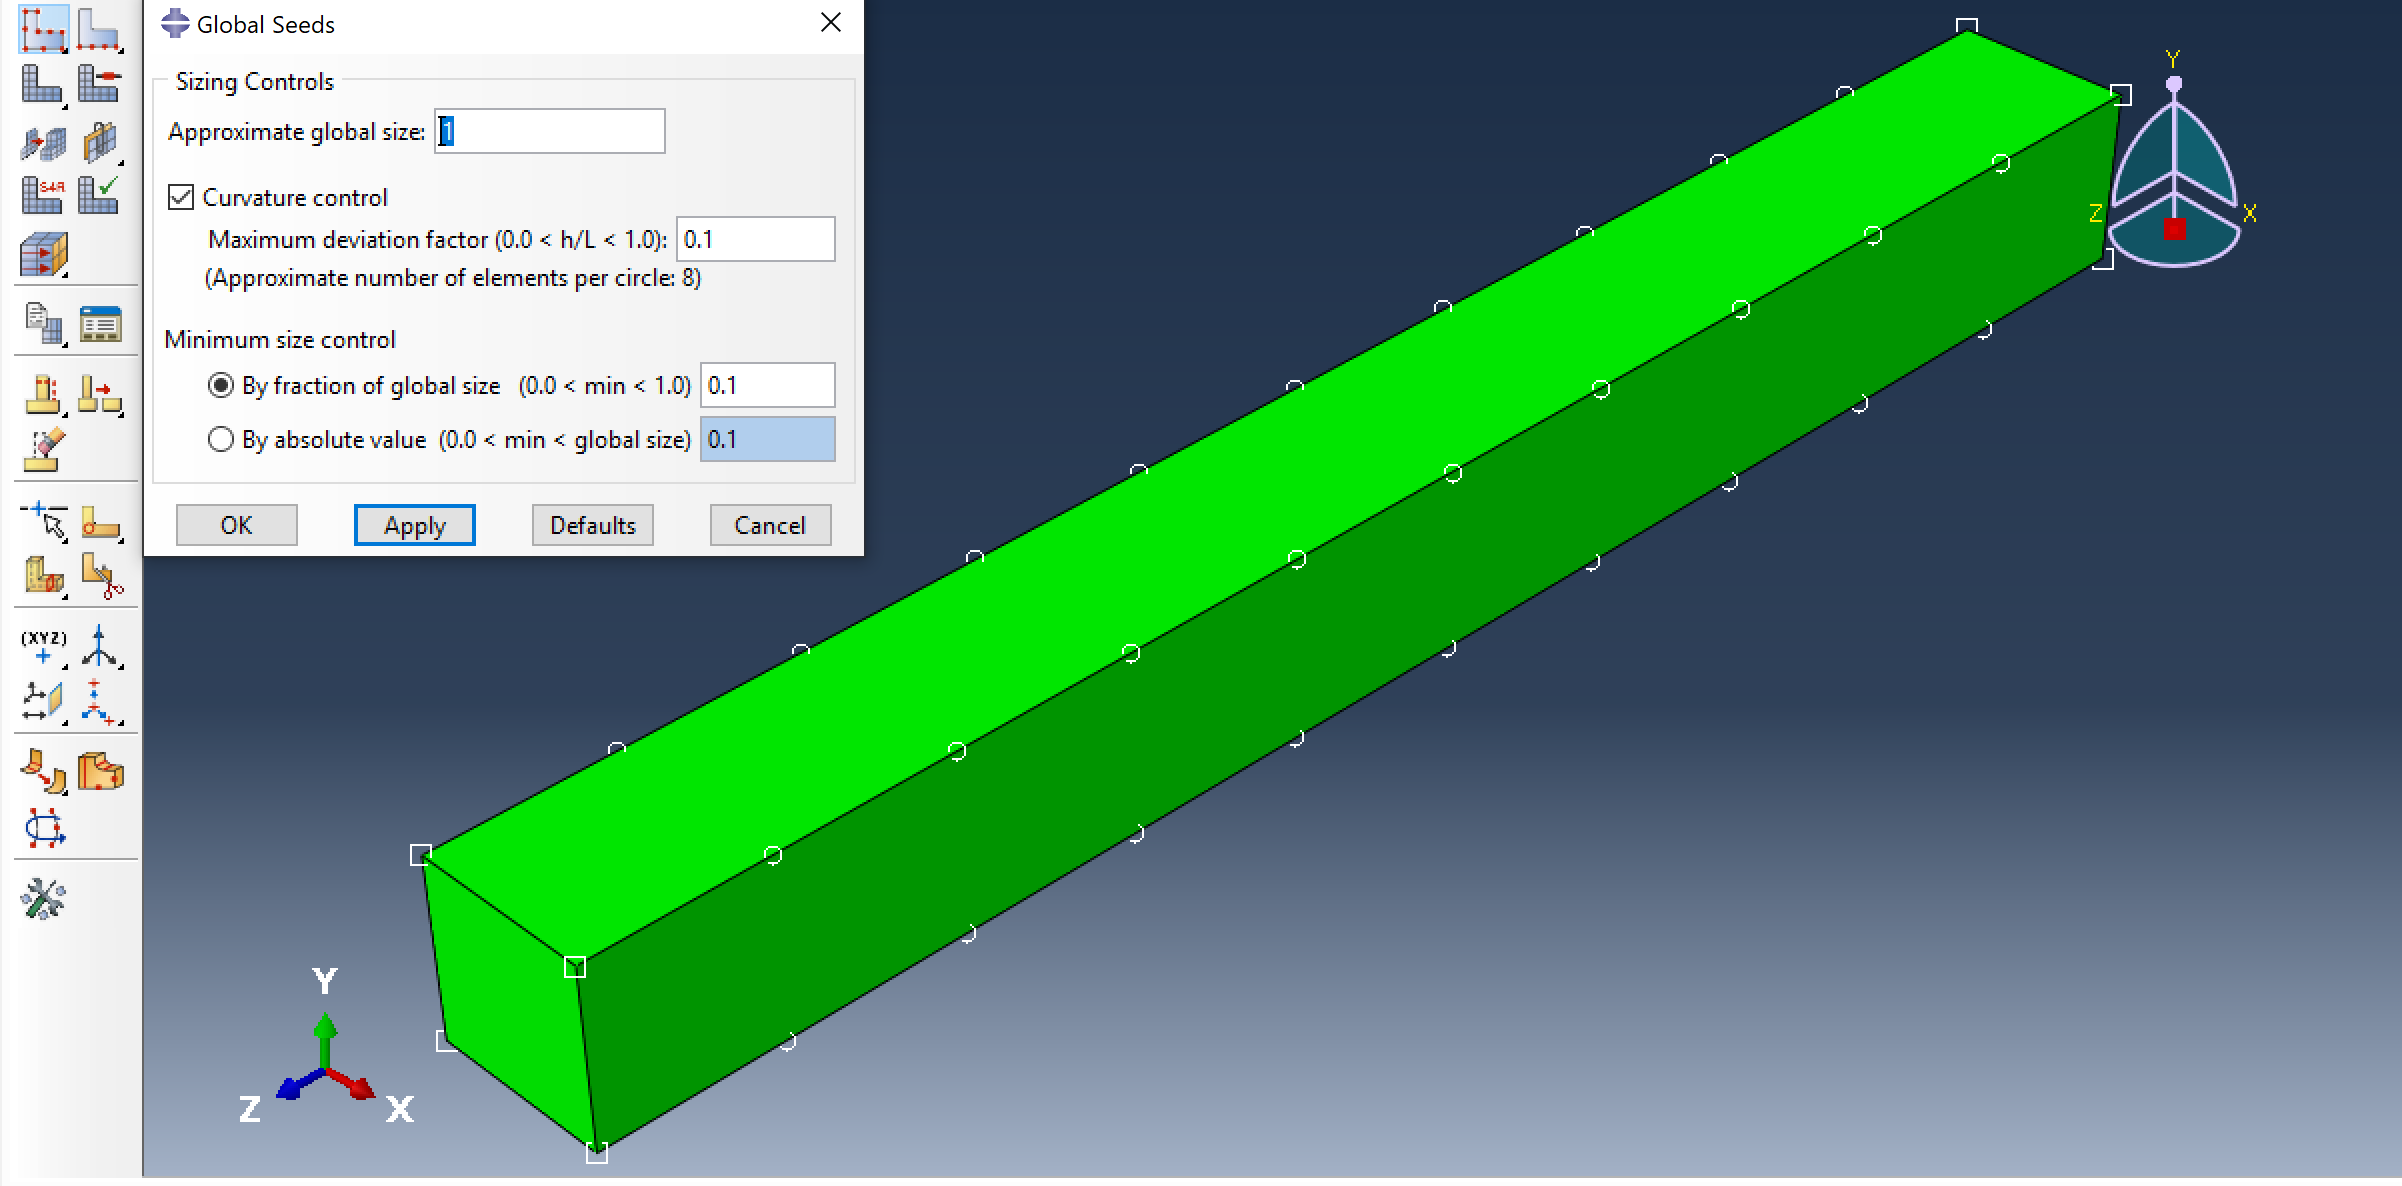
\includegraphics[scale=0.4]{capturas/mesh1.png}
\caption{``Global Seeds''}
\label{fig:mesh1}%
\end{figure}

\begin{figure}[h!tp]
\centering
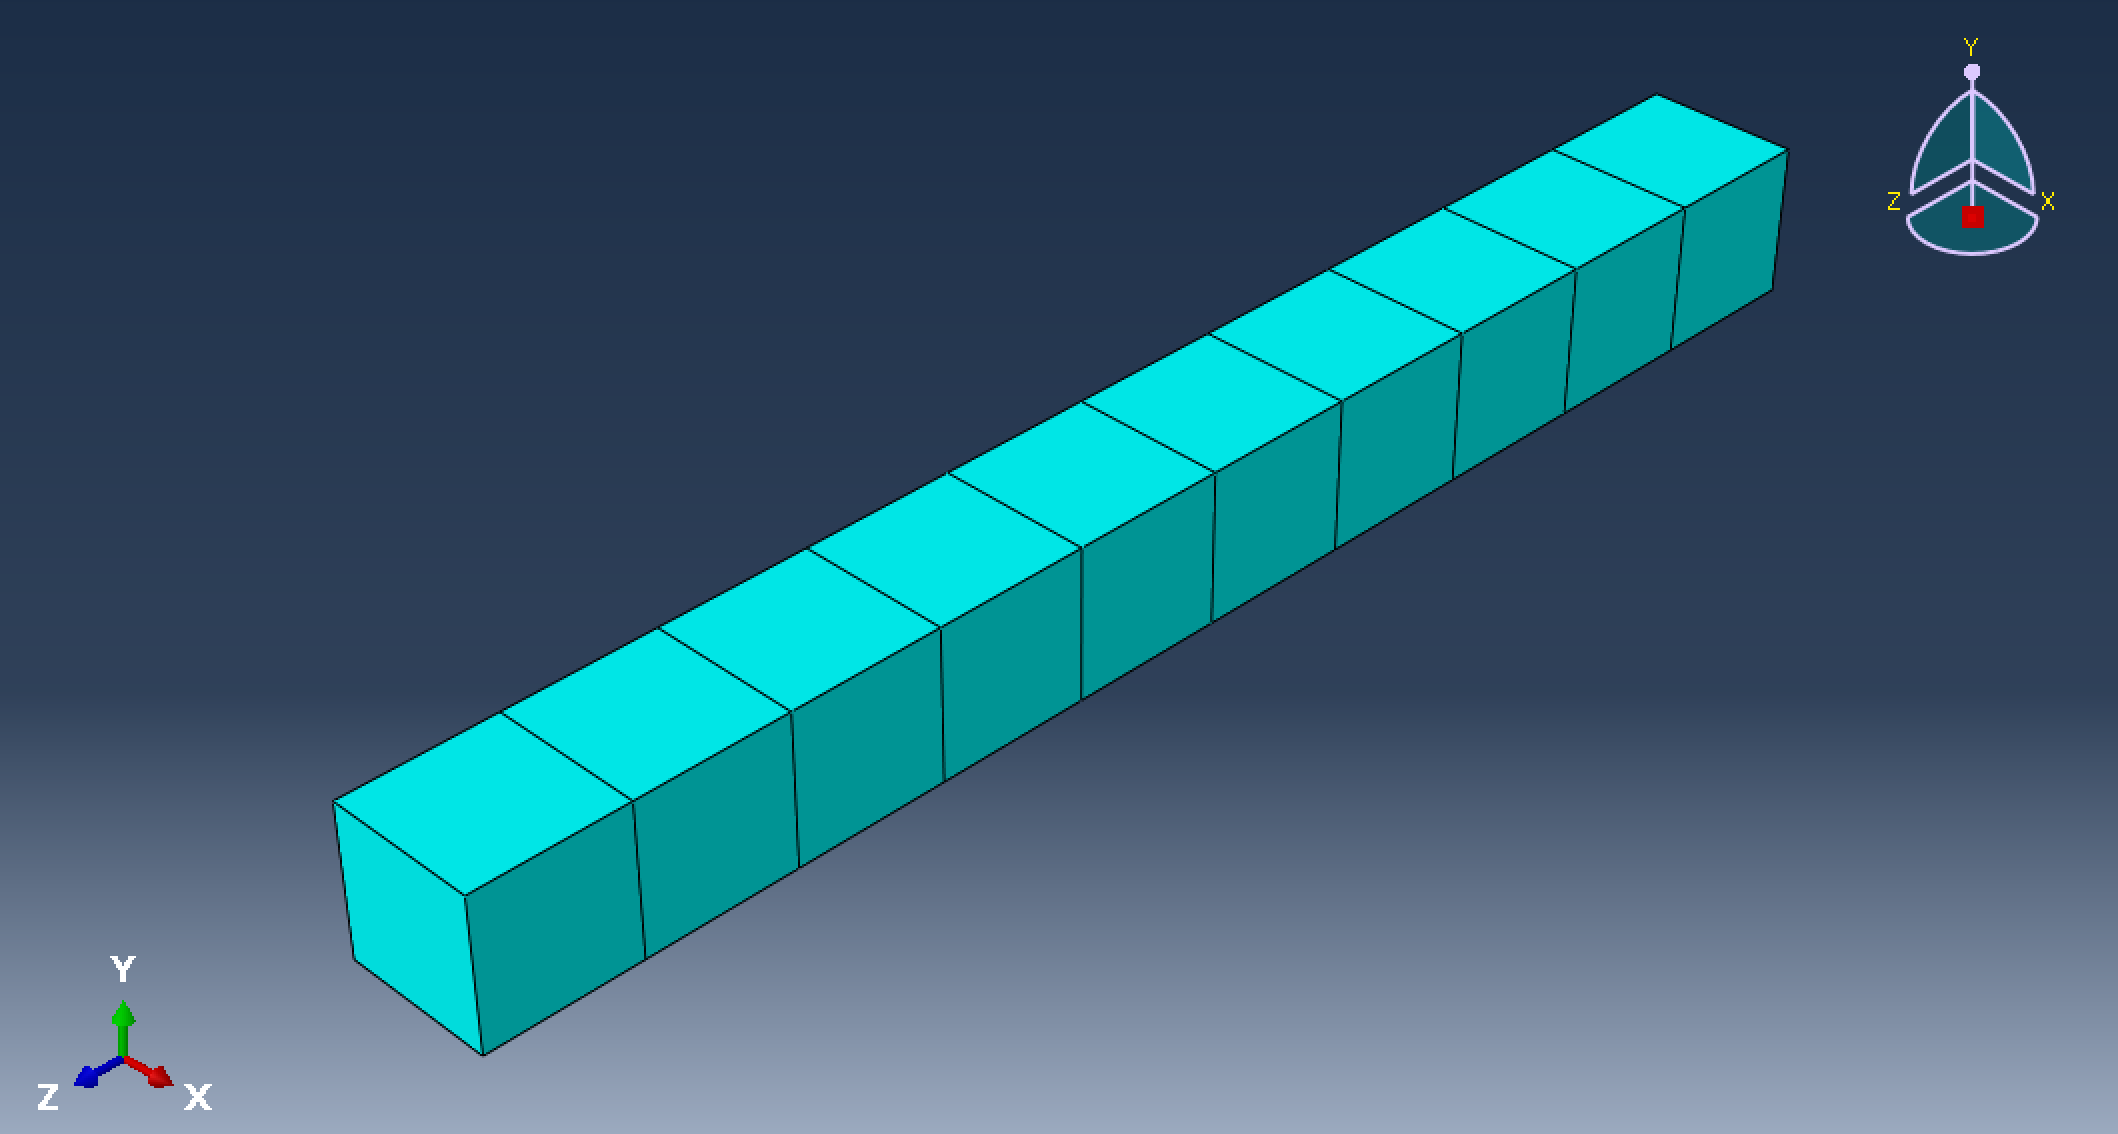
\includegraphics[scale=0.4]{capturas/mesh2.png}
\caption{Proposed mesh.}
\label{fig:mesh2}%
\end{figure}

\clearpage
\subsection{The \texttt{Job} module}

Now that the model is finished, a ``Job'' with the default analysis options is created
(figure \ref{fig:job-create}).
\begin{figure}[h!tp]
\centering
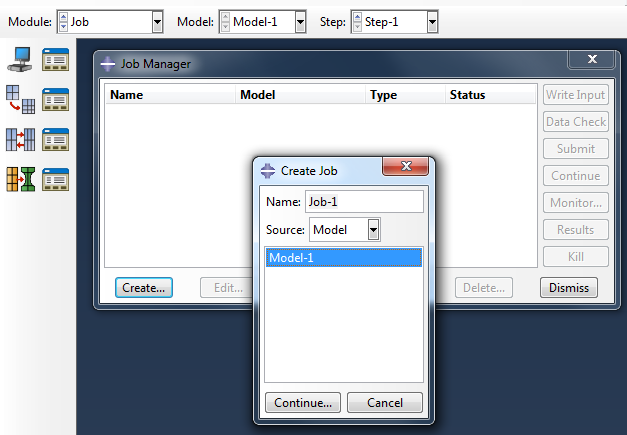
\includegraphics[scale=0.5]{capturas/37-job.png}
\caption{``Job'' definition}
\label{fig:job-create}
\end{figure}

This Job is submitted for analysis by clicking ``Submit''. The \emph{Status} changes from ``Submitted'' $\to$ ``Running'' and then $\to$ ``Completed'' if there is no error. 
(figure \ref{fig:job-submit}). It is always advisable to check for warnings in the ``Monitor''.
\begin{figure}[h!tp]
\centering
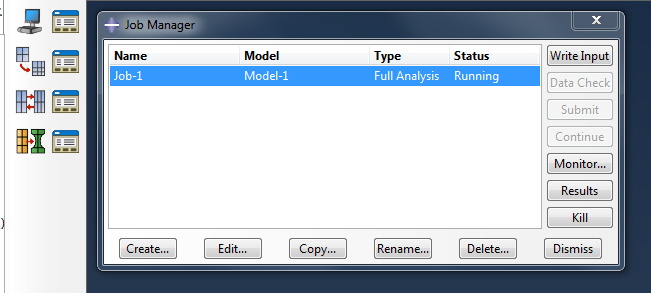
\includegraphics[scale=0.5]{capturas/38-job.png}
\caption{``Job'' submission}
\label{fig:job-submit}
\end{figure}

If there is no error message you can visualise the results.

\clearpage
\subsection{The \texttt{Visualization} module}

In order to check, the first field to visualise is the displacement in the along-bar direction Z. The peak displacement is 0.073 mm (figure \ref{fig:U}). We will plot the Z displacement with respect of the coordinate Z along the bar. 

\begin{figure}[h!tp]
\centering
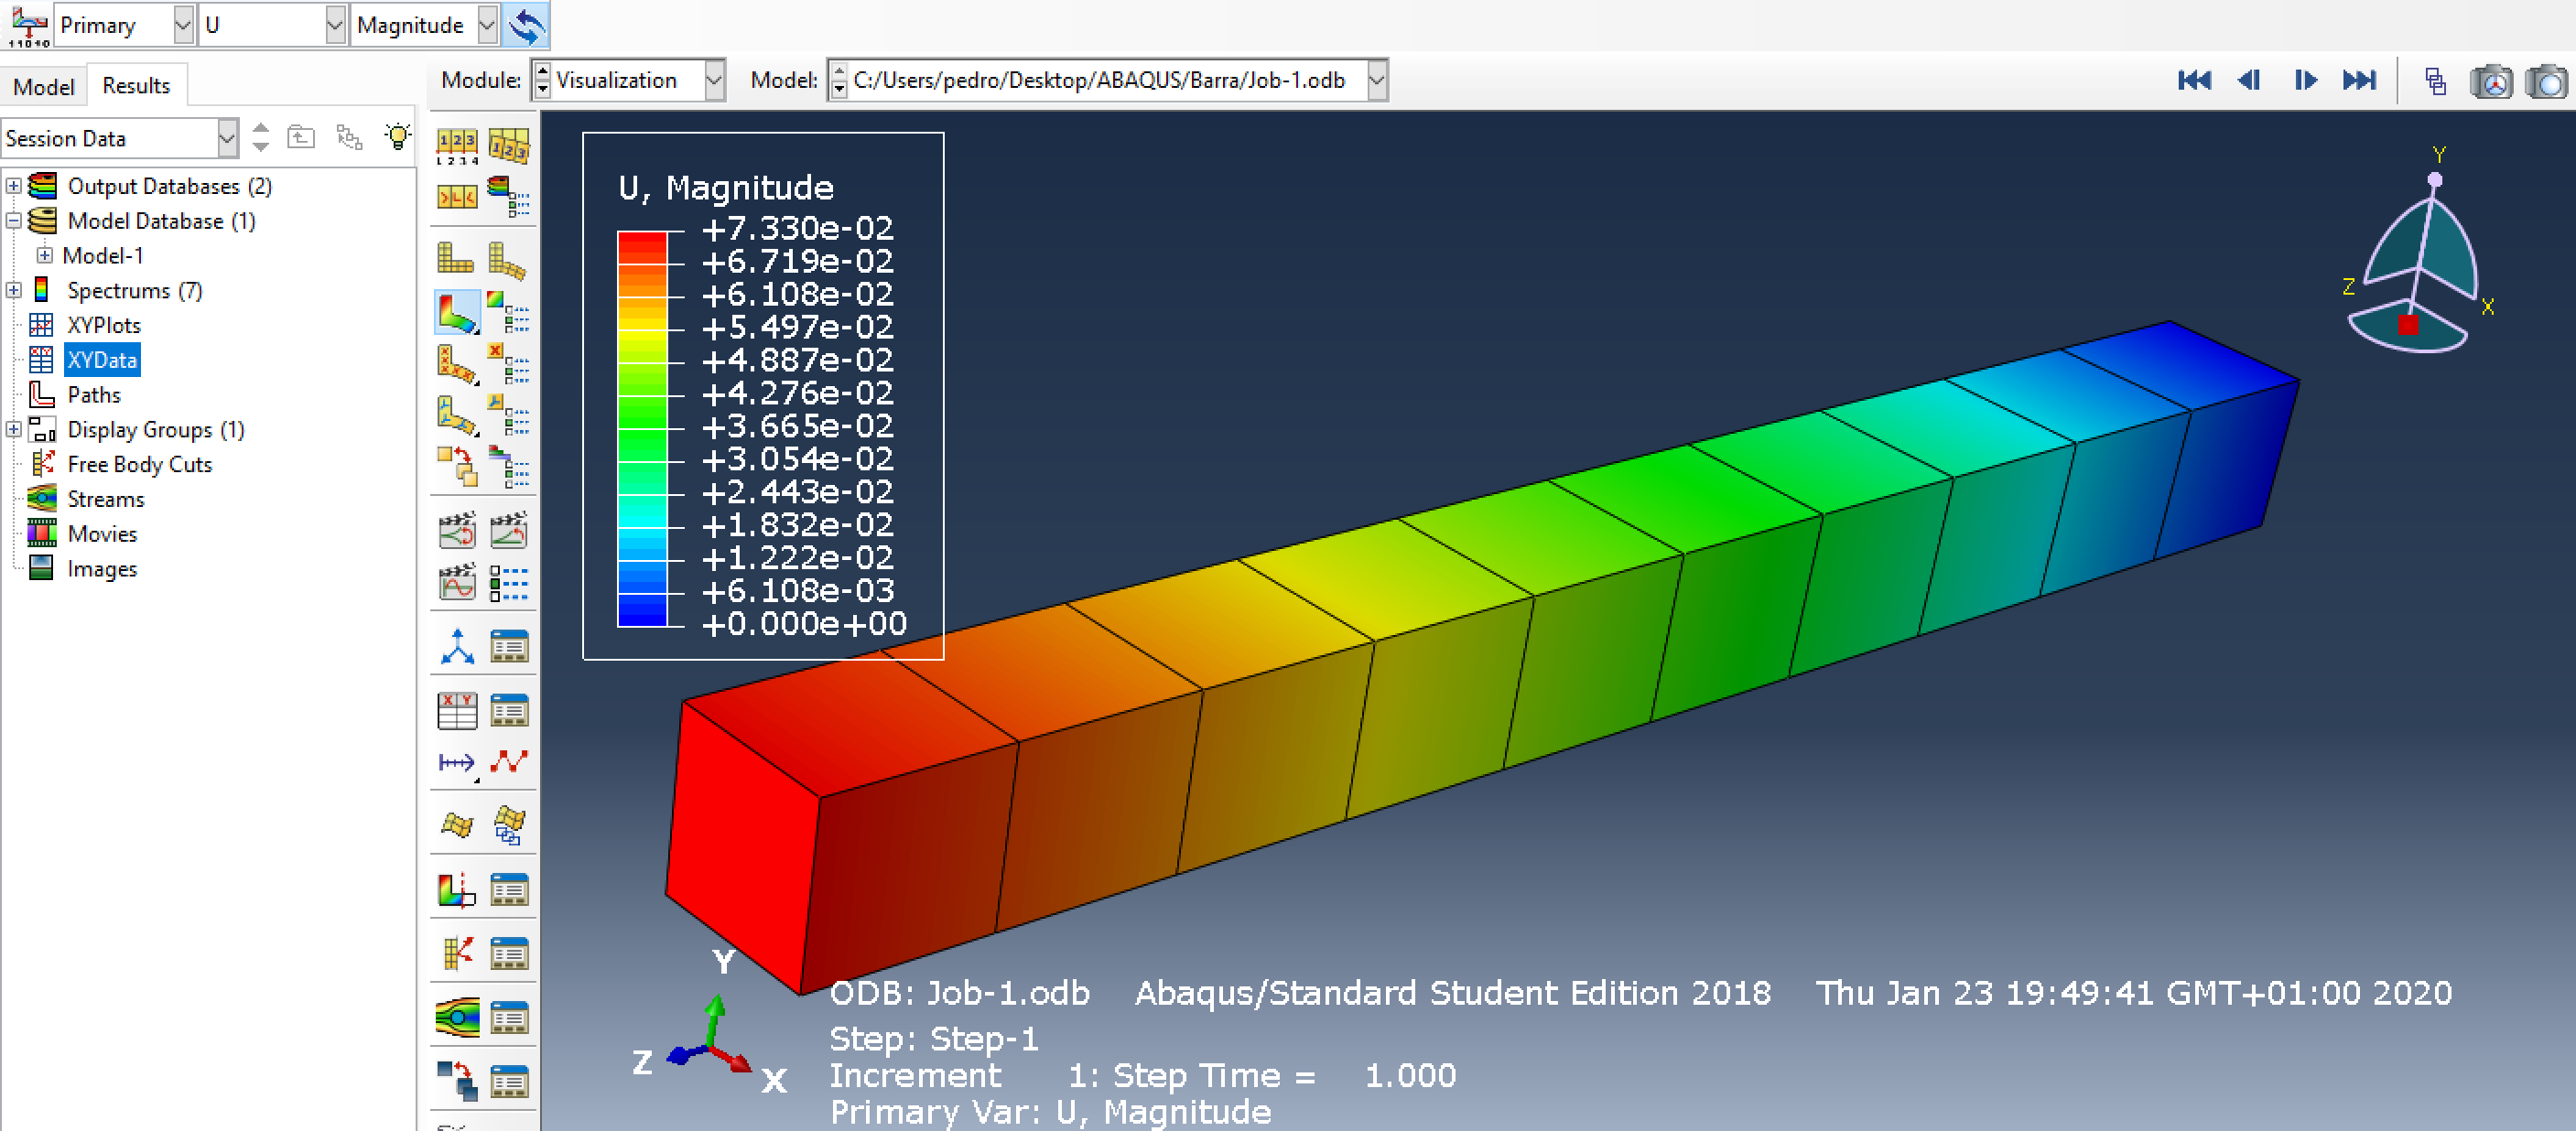
\includegraphics[scale=0.35]{capturas/res1.png}
\caption{Displacement field.}
\label{fig:U}%
\end{figure}

The first thing we need to do is to indicate the \emph{Path} (recall the first lab session) with two nodes distributed in \emph{Z}. We select `path' and with a right-click of the mouse we open a menu where we select \emph{create} (figure \ref{fig:path}). The type of path will be based on a selection of the nodes. Our mode of selection will be advancing in the positive-Z direction, therefore we chose \emph{Add After} and make sure that we select a node in the face $Z=0$ and the next one in $Z=L$. We can chose any edge because all of them have the same response. This defines the path as shown in figure \ref{fig:path2}.

\begin{figure}[h!tp]
\centering
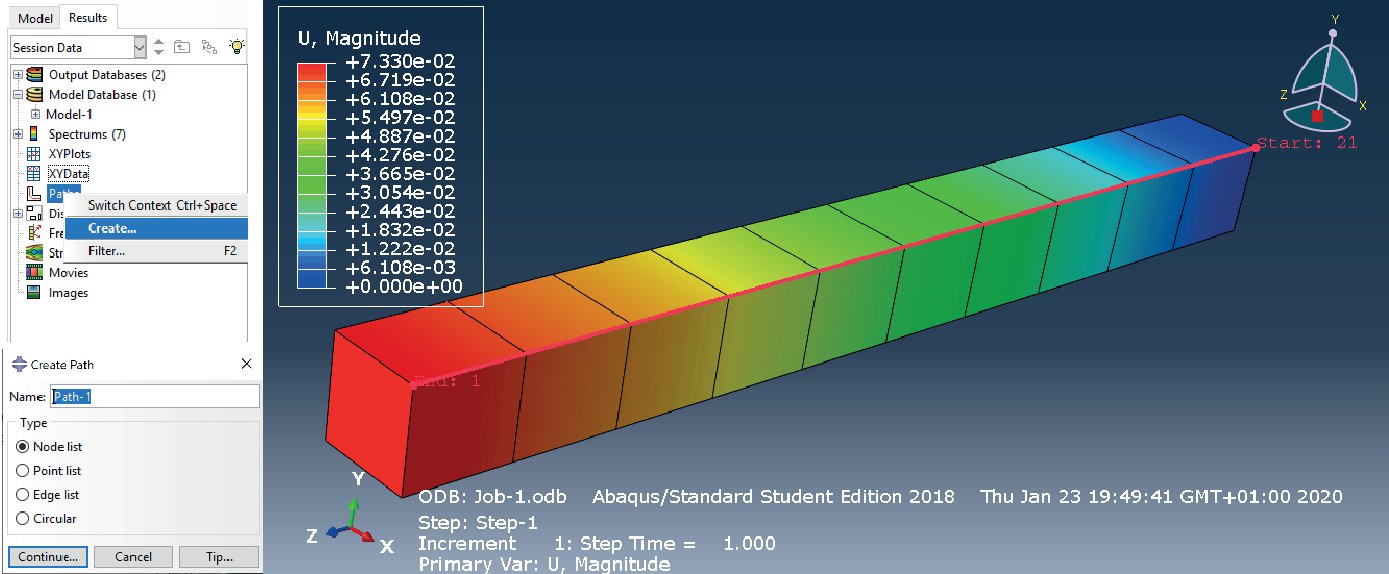
\includegraphics[scale=0.75]{capturas/path.pdf}
\caption{Path definition.}
\label{fig:path}%
\end{figure}
\clearpage

\begin{figure}[h!tp]
\centering
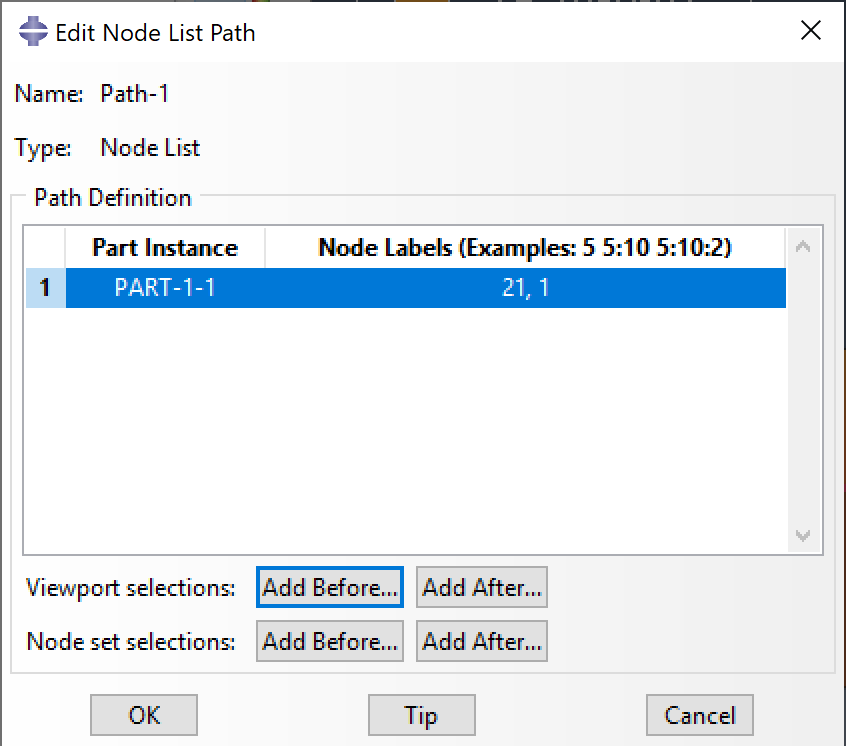
\includegraphics[scale=0.55]{capturas/path2.png}
\caption{Node list in the path.}
\label{fig:path2}%
\end{figure}

Now we can create a graph with the along-bar displacement ($U_Z$) in the structure. We need to go to \emph{XY-Data} and in this field, with a right-click of the mouse a menu opens. There we select \emph{Create} and select a displacement field $U3$, which corresponds to the along-bar displacement ($U_Z$). In the window \emph{XY Data from Path} (figure \ref{fig:Data1}) we chose the Path defined previously (in the undeformed configuration) and select the option to include intersections because this will add the intermediate nodes along the start and end nodes of the path. Finally, we select the horizontal axis in our plot as the coordinate Z.

\begin{figure}[h!tp]
\centering
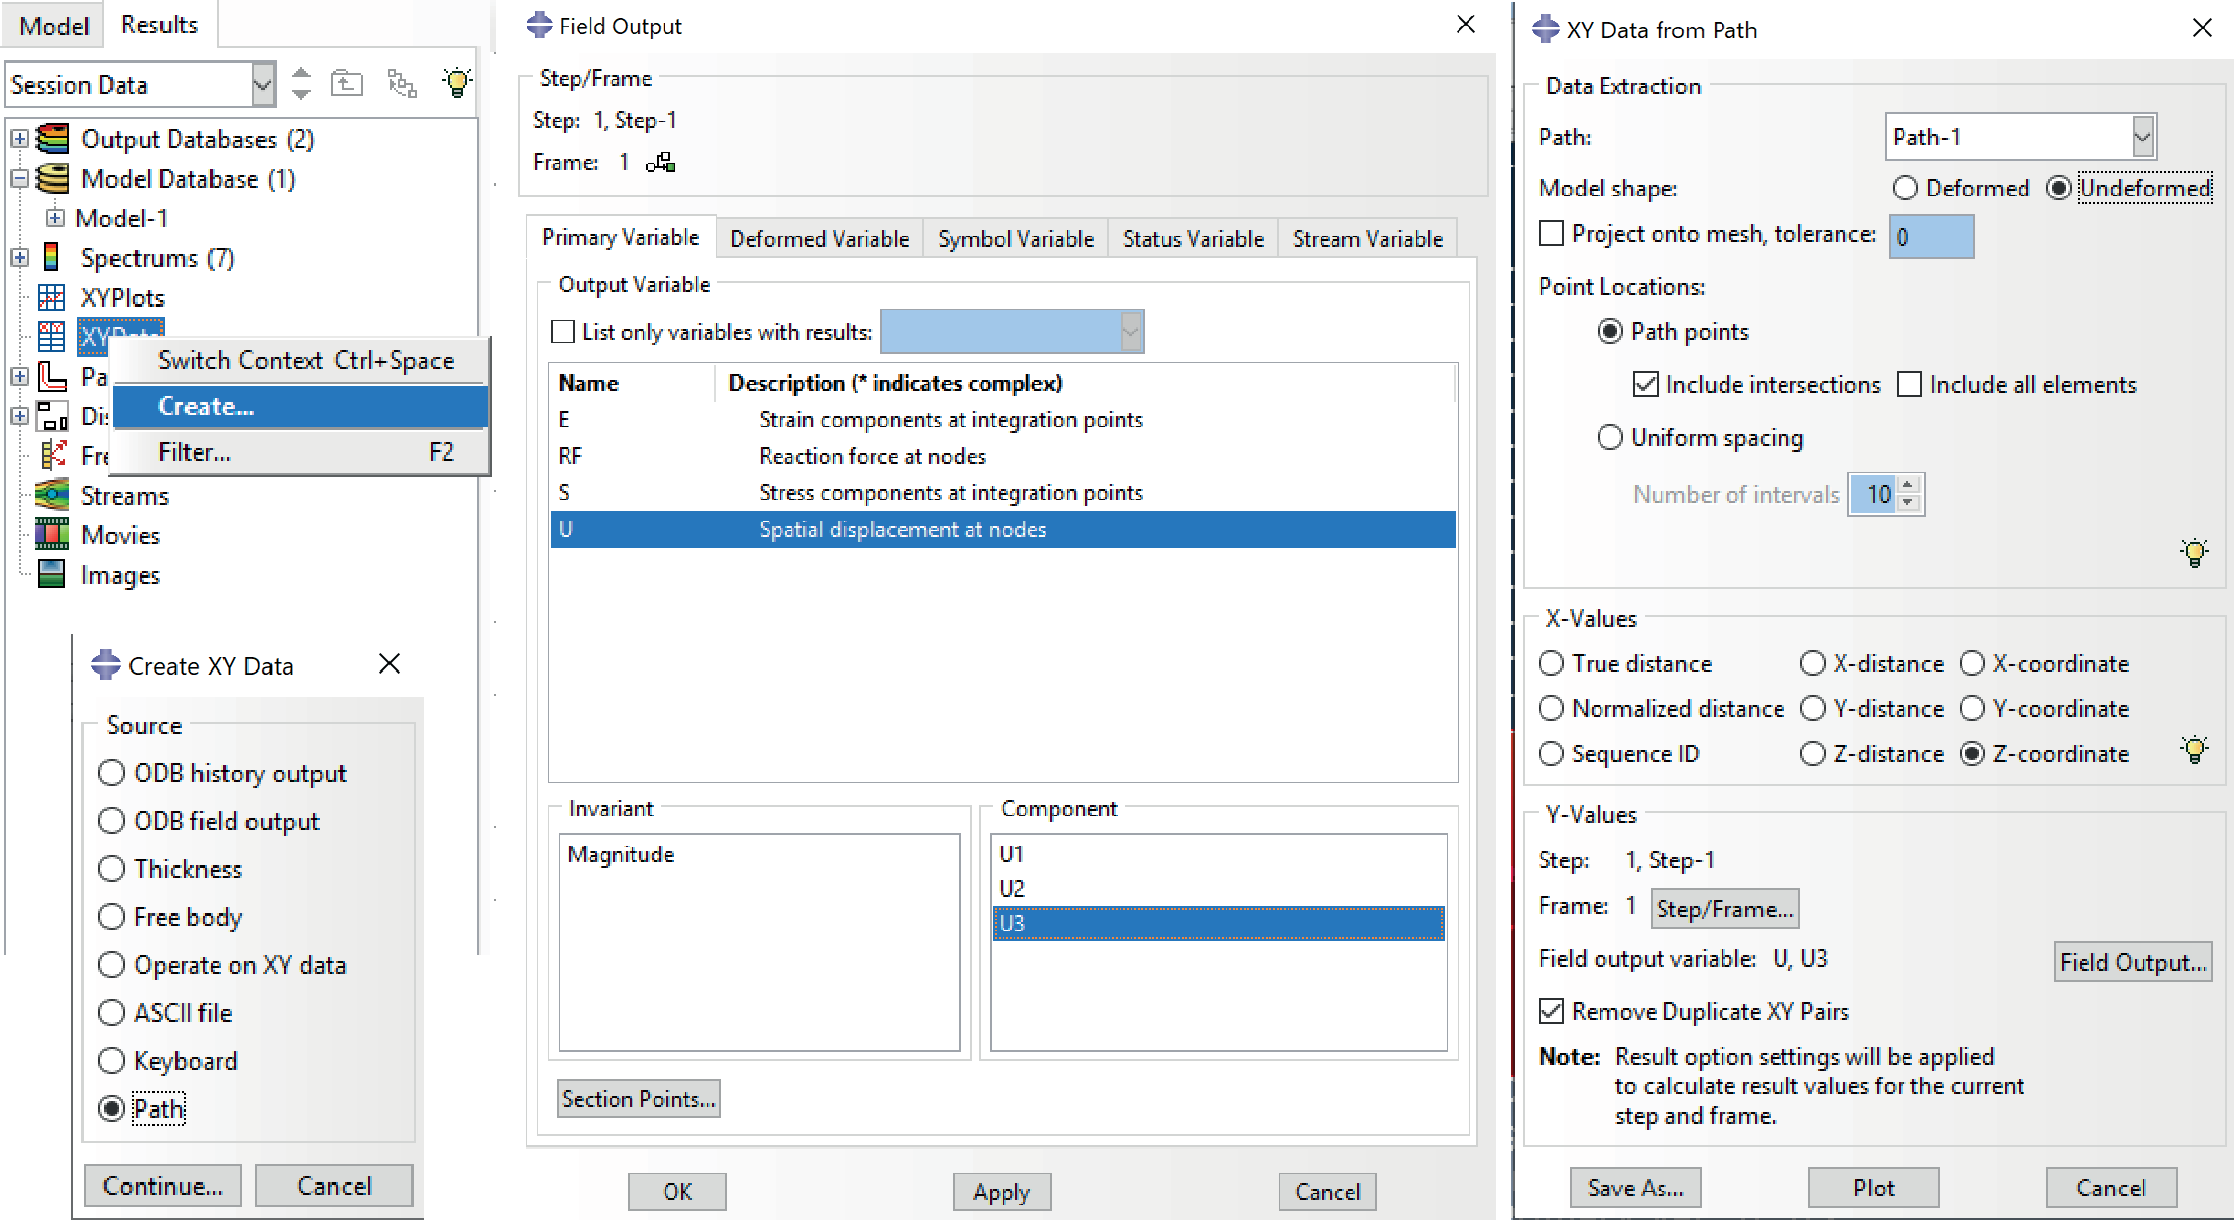
\includegraphics[scale=0.45]{capturas/U-data.pdf}
\caption{Creation of the XY-data}
\label{fig:Data1}%
\end{figure}

Plotting this graph we should obtain figure \ref{fig:Data2}. We will compare this with the results obtained in the \texttt{Python} FE solver script.
\clearpage
\begin{figure}[h!tp]
\centering
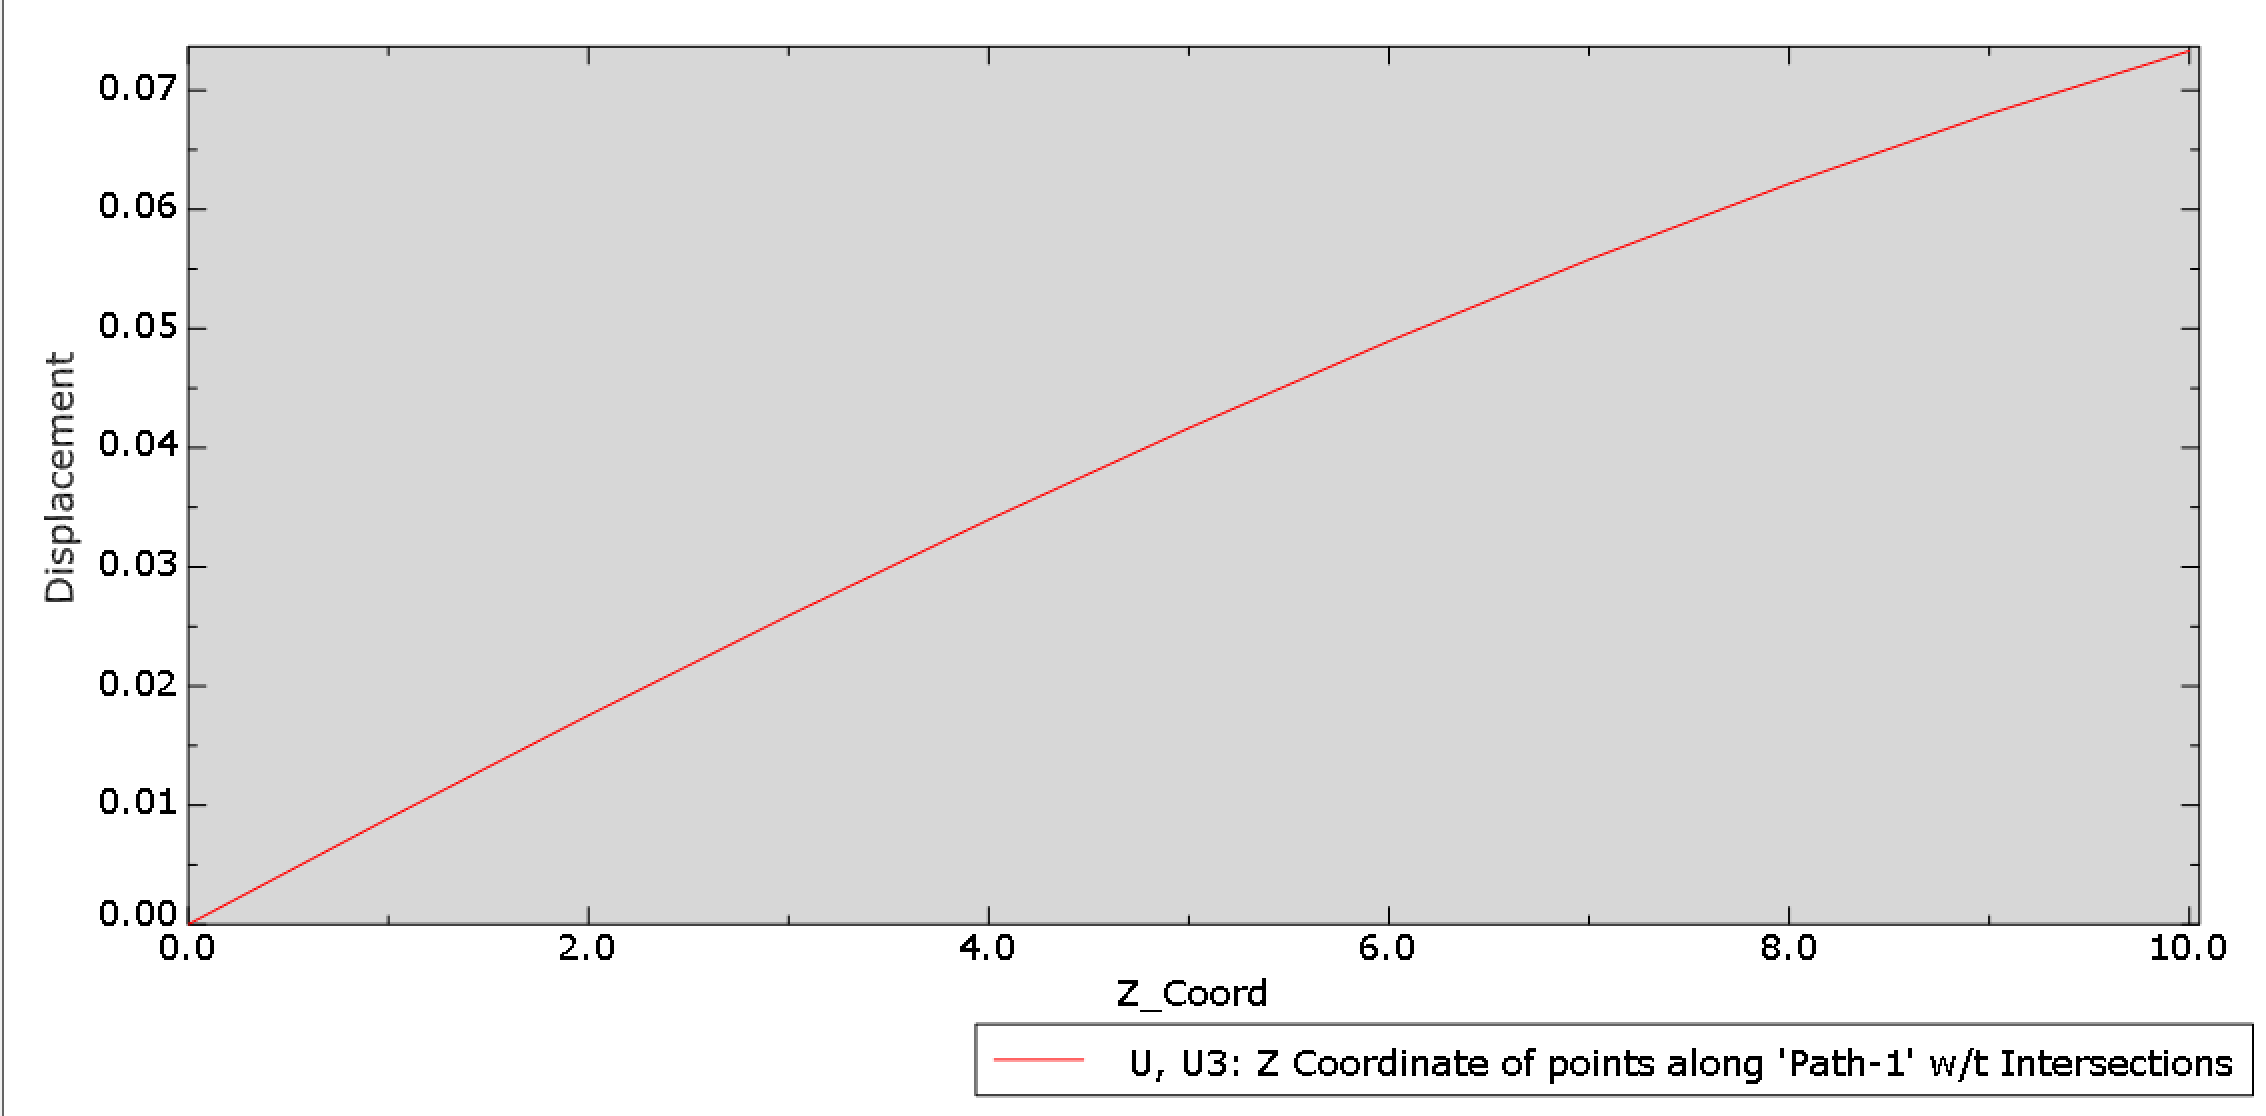
\includegraphics[scale=0.45]{capturas/U-data2.png}
\caption{Along-bar displacement obtained in Abaqus.}
\label{fig:Data2}%
\end{figure}

We will save this result to compare it later with that obtained in \texttt{Python} and with the analytical solution given by the strong formulation of the problem. This is done by clicking the icon \emph{Save as..}. We will call the file \texttt{u3.txt}. 

If we change the response field to stresses and plot S33, which corresponds to the normal stress $\sigma_z$ we will obtain a result similar to figure \ref{fig:Data3}.  You will observe that that the trend is to be expected but at the ends some strange things happen. This is because the stress is calculated at the integration points and not at the nodes, where the path is defined. Therefore the stress needs to extracted in a different way.

\begin{figure}[h!tp]
\centering
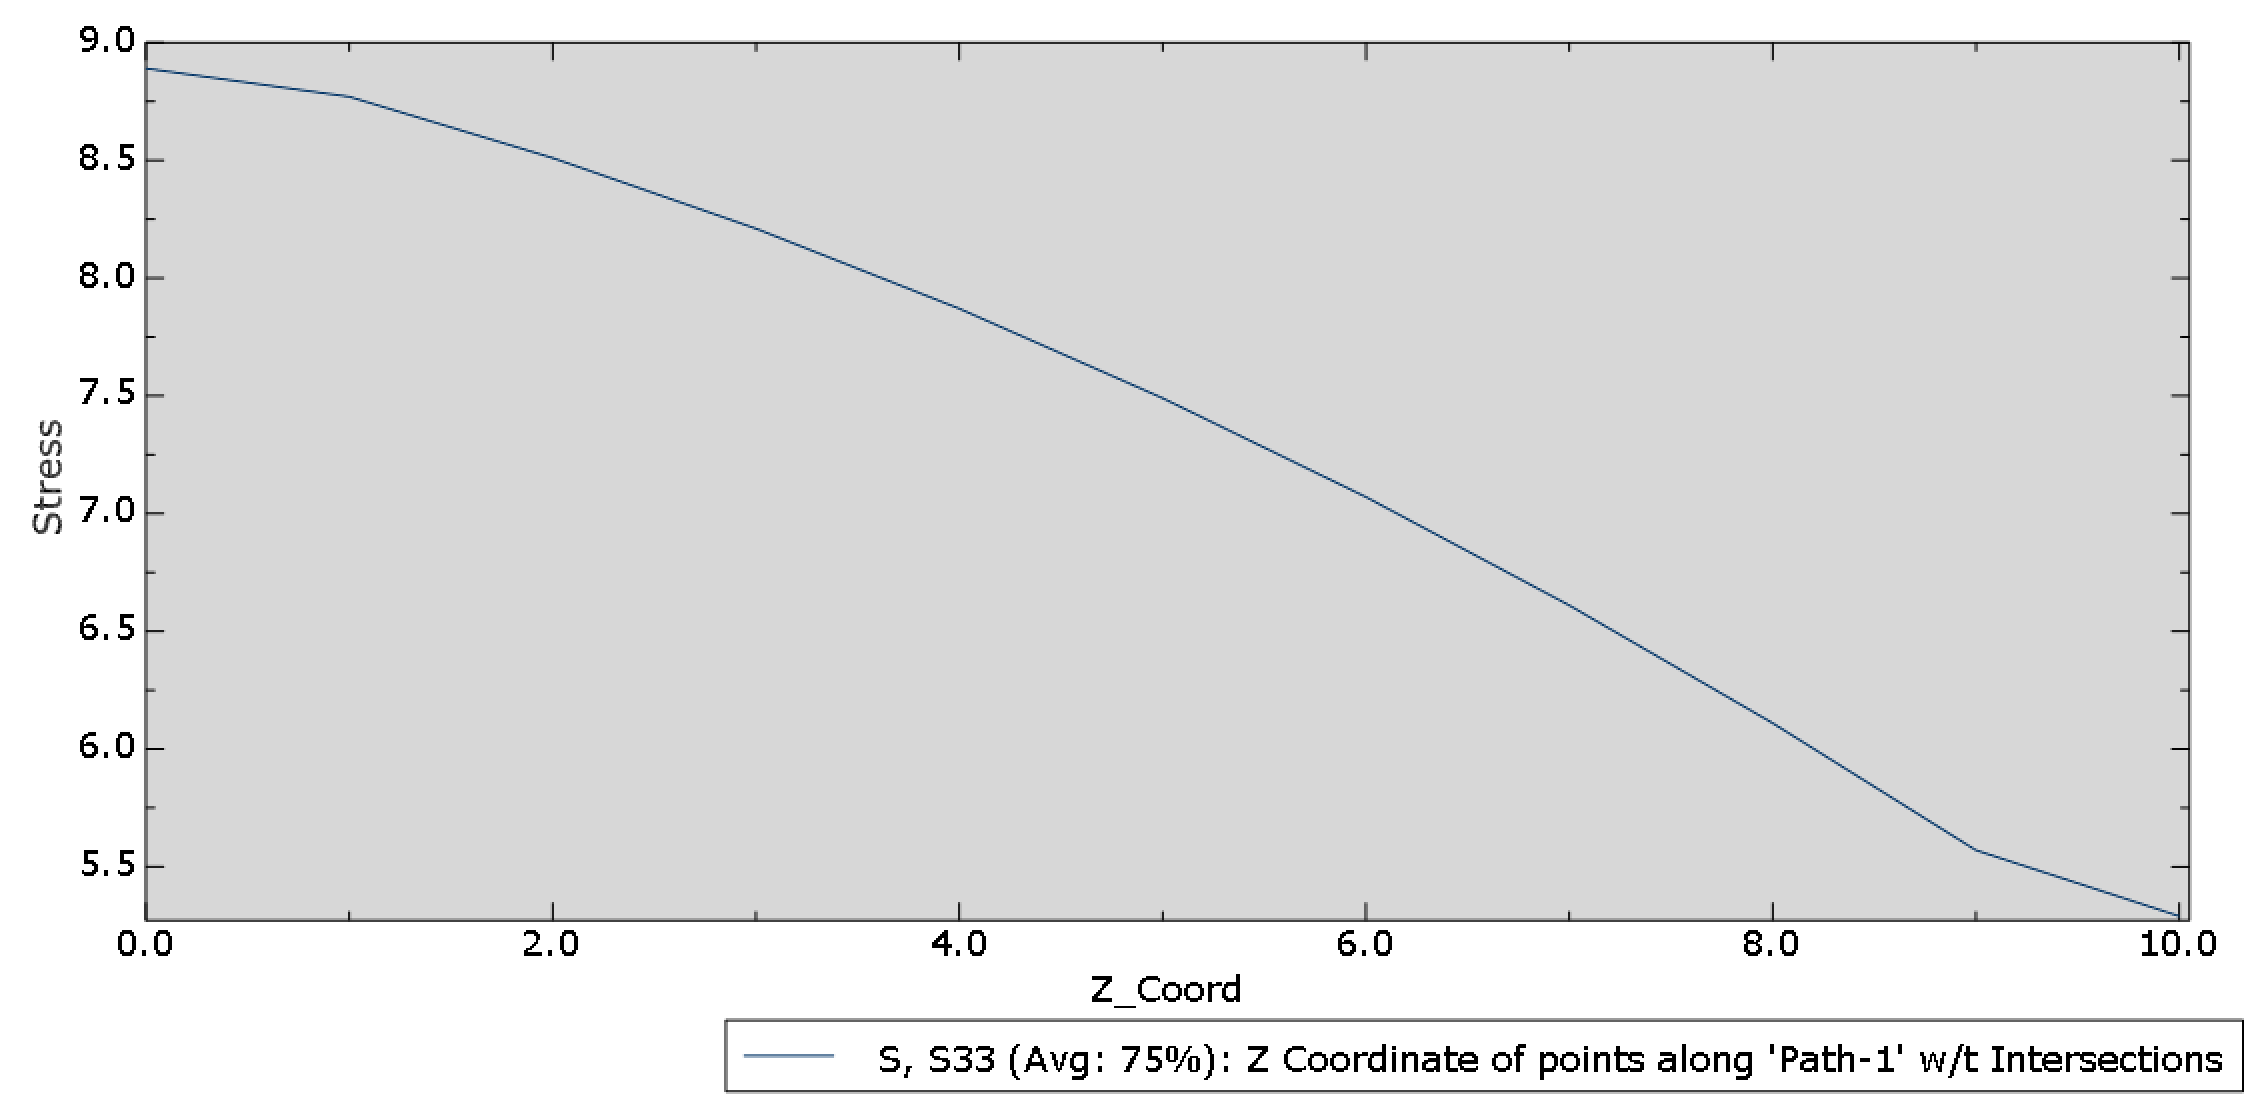
\includegraphics[scale=0.45]{capturas/S-data.png}
\caption{Stress $\sigma_z$ along the axis Z.}
\label{fig:Data3}%
\end{figure}

To this end we go to tab ``Report/'' and there we select the suboption \emph{Field Output}. This will open a wind with a tab called \emph{Variable} where we select the field output S33 at the integration points (figure \ref{fig:out1a}), while in the tab ``Setup'' we will specify the file name as \texttt{s33.csv} (figure \ref{fig:out1b}).

\begin{figure}
\centering
\captionsetup[subfigure]{justification=centering,singlelinecheck=false}
  \begin{subfigure}[b]{0.36\textwidth}
  \hspace{0mm}
    \imagebox{85mm}{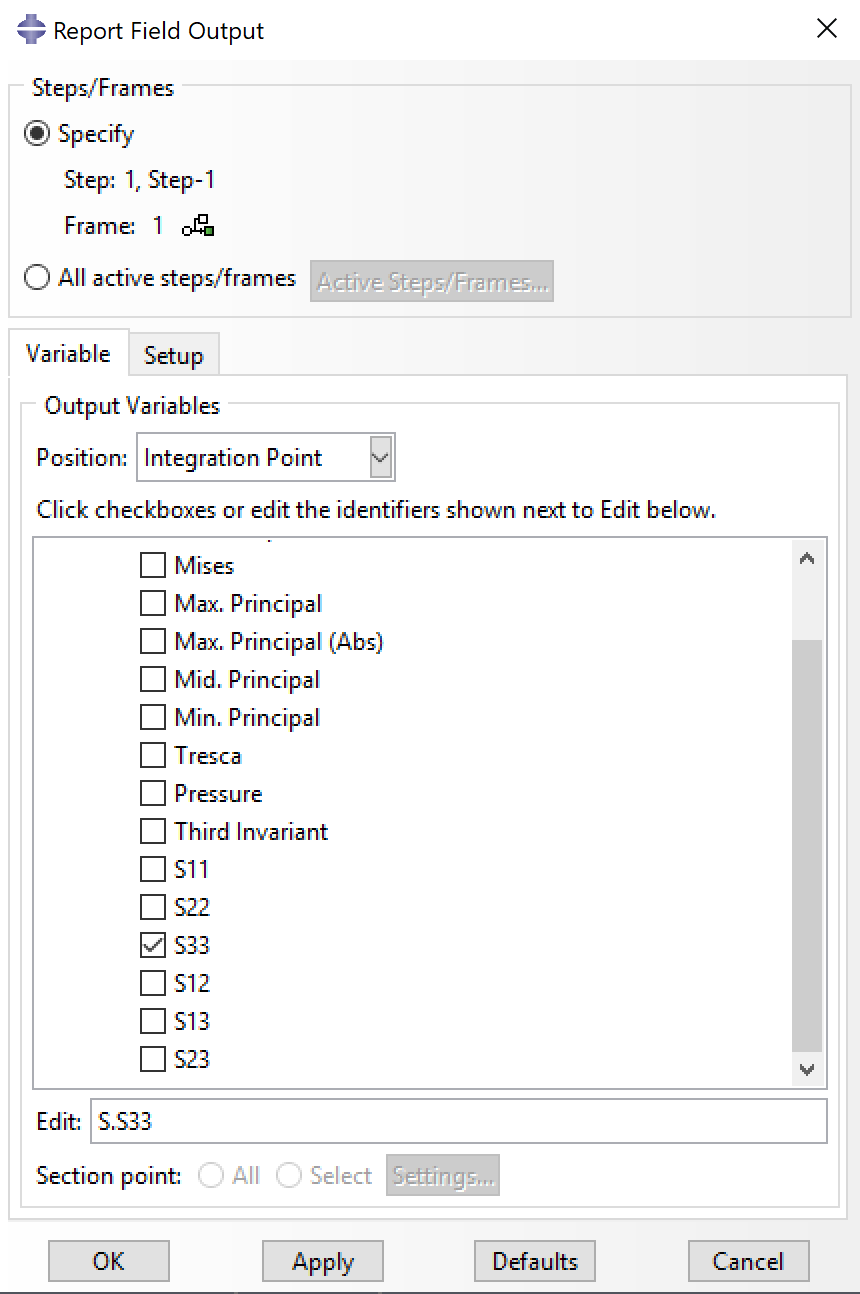
\includegraphics[scale=0.35]{capturas/out1.png}}
    \caption{Variable\label{fig:out1a}}
  \end{subfigure}
  \begin{subfigure}[b]{0.36\textwidth}
  \hspace{5mm}
    \imagebox{85mm}{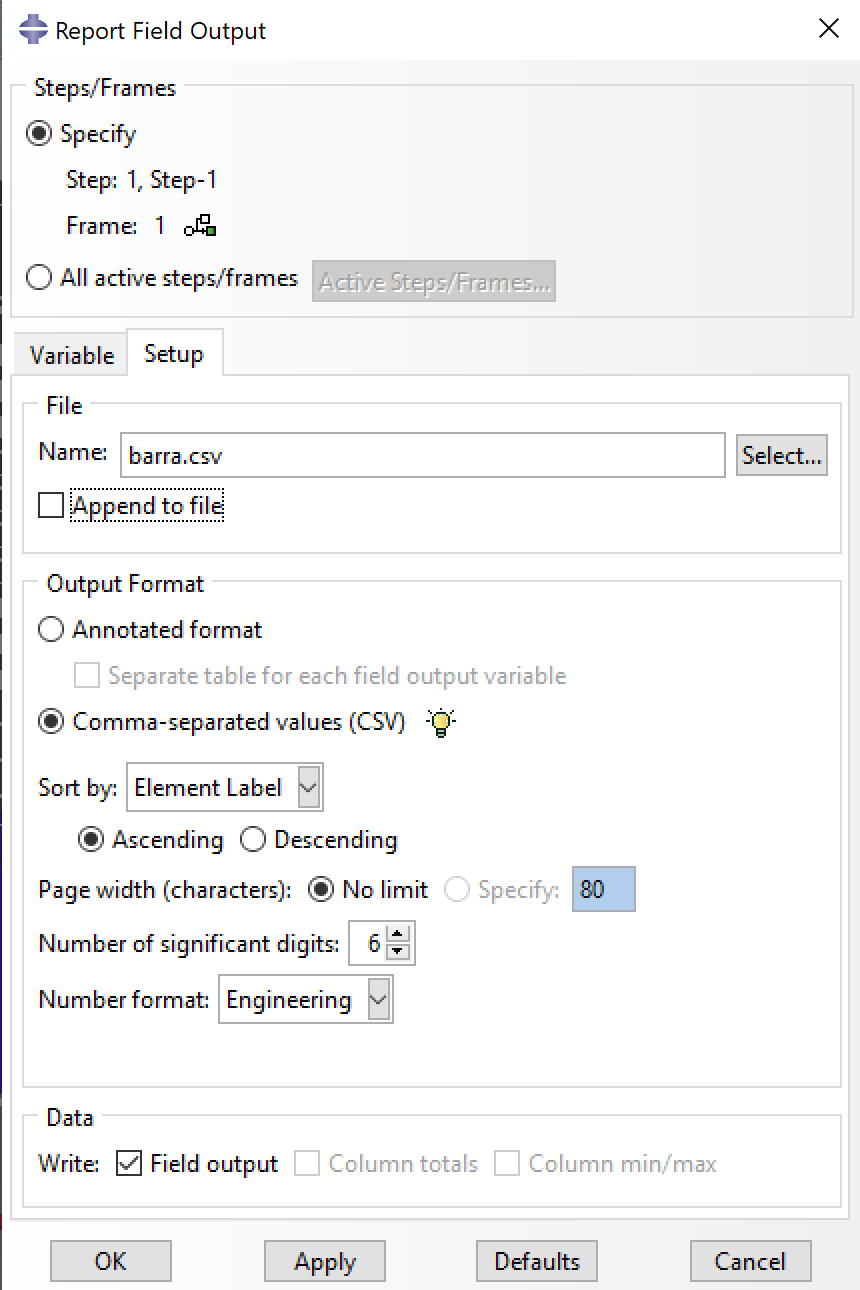
\includegraphics[scale=0.35]{capturas/out2.png}}
    \caption{Setup\label{fig:out1b}}
  \end{subfigure}
\caption{Field Output}
\label{fig:out1}
\end{figure}

\clearpage
\section{Example of finite element code in Python}
\label{sec:python}

In the following link we provide a \emph{Notebook} of \emph{Python} with a FE code applied to the case of a 1D elastic bar.

The file \texttt{*.ipynb} can be downloaded from the repository below,\\

\href{https://github.com/juanjosearribas/met_comp}{\textcolor{blue}{\texttt{Repositorio Git-Hub}}}\\

or alternatively it can be open directly in any of the programs that will be detailed now. The \emph{Notebook} can be run with the program \texttt{Jupyter}, which belongs to the suite \texttt{Anaconda}, open for plataforms \emph{Windows, Mac y Linux}. It is necessary to download this suite and load the \emph{Notebook}, either opening the file with extension \texttt{*.ipynb}, or from the repository in Git-Hub mentioned previously.

Another option is to run the script \emph{in the cloud}, without the need to install anything. Some of the most widely used are:

\begin{itemize}
\item  \href{https://colab.research.google.com}{\textcolor{blue}{\texttt{Colab de Google}}} It is necessary to have a gmail account.
\item  \href{http://mybinder.org/}{\textcolor{blue}{\texttt{MyBinder}}} Only available from a repository in Git-Hub
\end{itemize}

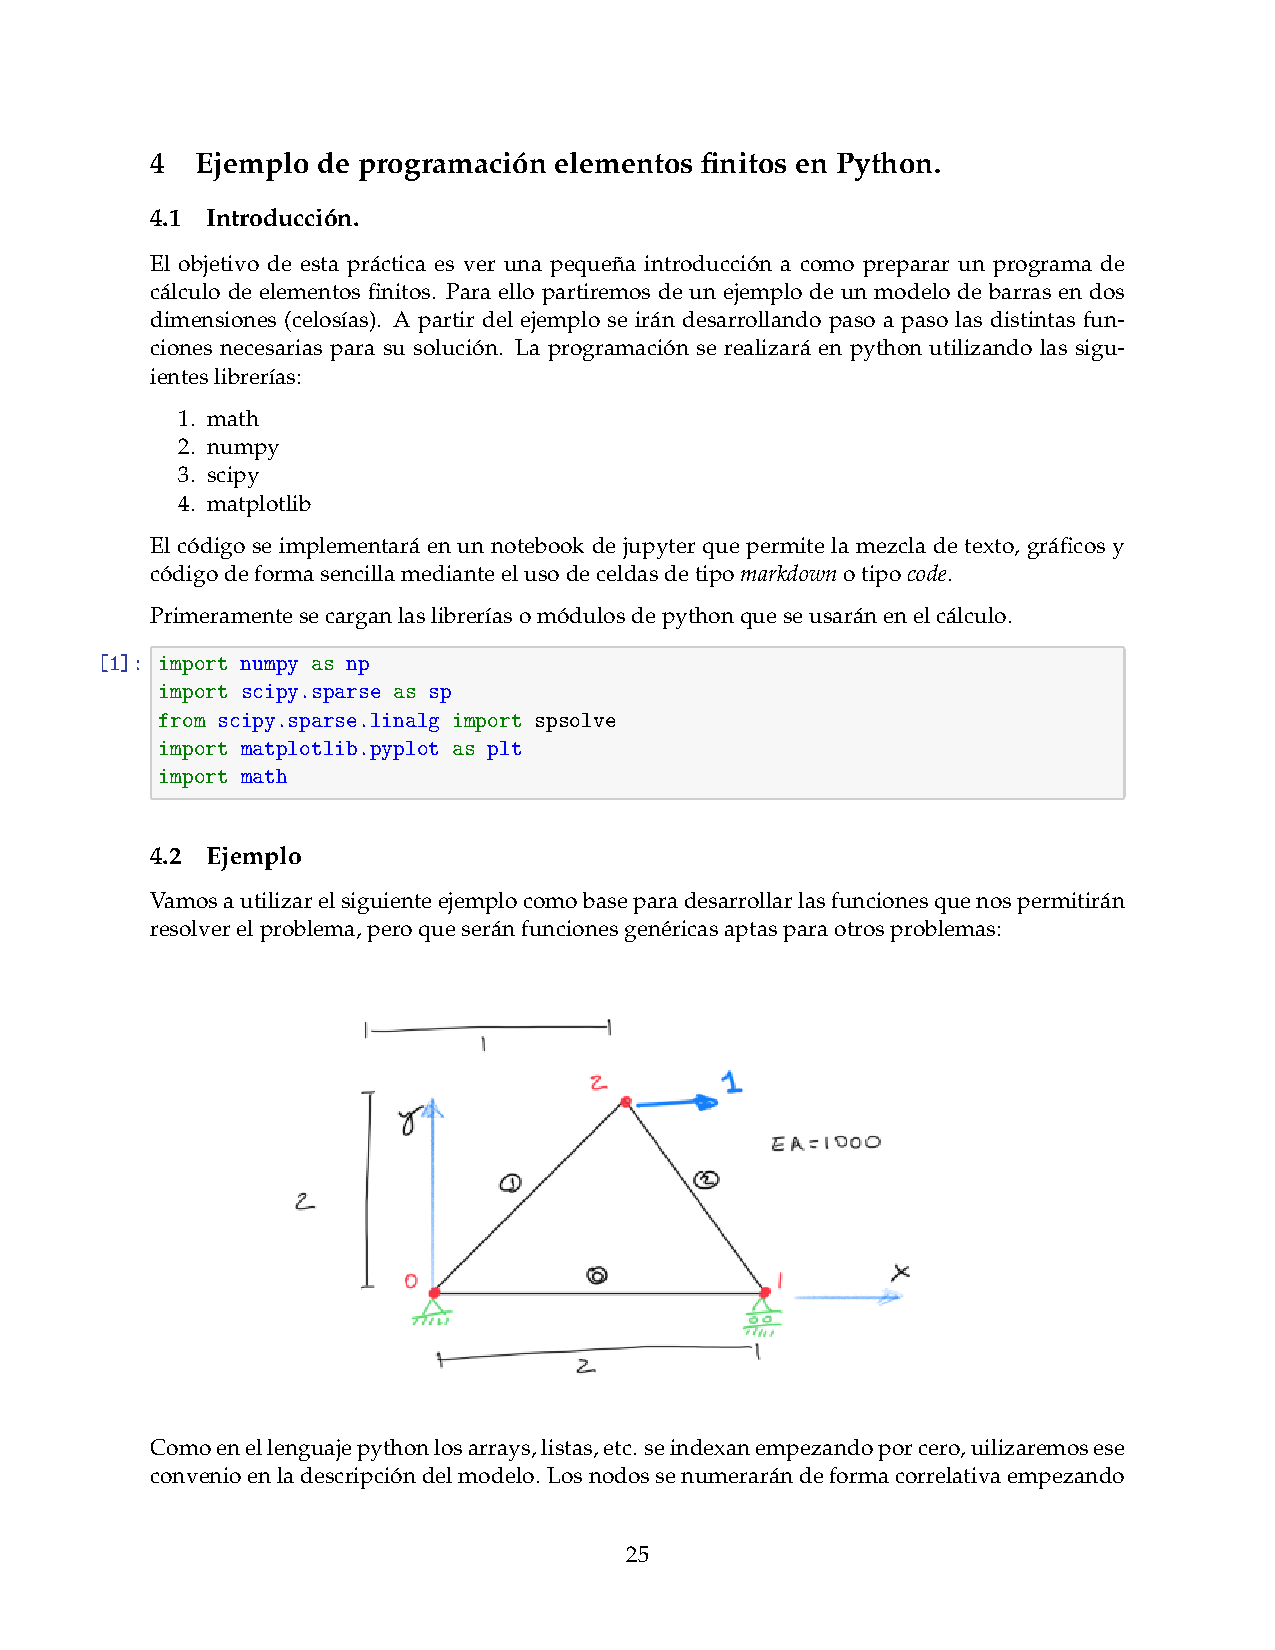
\includepdf[pages=-]{python_to_tex/el_fin2d_OK}


\clearpage
\appendix
\numberwithin{equation}{section}
\section{Simulation with MatLab / Octave}
\label{sec:matlab}

We give here the same code developed in \texttt{MatLab} for those of you familiar with this programming language (or with the opensource program \texttt{Octave}).

\subsection*{Código MatLab / Octave}
\label{sec:esq}

The organisation of the \texttt{Matlab} / \texttt{Octave} code is free. However, given that this is the first contact of the student with FE coding, it is recommended to follow some patterns.


\begin{itemize}
\item Pre-process

In the pre-processing we define the material, geometry of the structure, boundary conditions and finite element discretisation (mesh). Depending on the type of problem we may need to define also the total number of degrees of freedom.


\begin{lstlisting}[ label=codigo1,caption=Matlab scheme \emph{(a)}]
% Definition of the parameters for each student:
Nmat=1124                      % Registration number of the student 
m=floor(Nmat/1000)             % Thousands
c=floor((Nmat-m*1000)/100)     % Hundreds
d=floor((Nmat-m*1000-c*100)/10) % Tens
u=Nmat-m*1000-c*100-d*10       % Units

% A: PRE-PROCESS
%----------------------------------------------------------------

% 1. Geometry
A=1;              % Area
L=10;             % Length of the bar

% 2. Material
E=1000;           % Young's modulus

% 3. Forcing boundaries
P=5;                % Force applied at en x=L
q0=d/10;            % Value of the volumetric force at x=0
qf=q0+u/10;        % Value of the volumetric force at x=L

% 4. Mesh
Nele=11-c;          % Number of elements
Nnod=Nele+1;        % Number of nodes
q=linspace(q0,qf,Nnod);
h=L/Nele;           % Length of each element

% 5. Number of degrees of freedom
% Dim = GDL total = degrees of freedom of each node x number of nodes
gdl=1;
Dim=Nnod*gdl;

\end{lstlisting}

\item Solver - construction of the element and global matrices

The first part of the \textit{solver} builds the global stiffness and forcing matrices from the elementary ones. The elementary stiffness matrix is the same for all the elements because they have the same material and dimensions. However, the volumetric force varies along the bar. In addition, the last node (right end) has an applied force 5 N.

\begin{lstlisting}[ label=codigo2,caption=Matlab scheme \emph{(b)}]
% B: CONSTRUCTION of GLOBAL MATRICES and VECTORS 
%----------------------------------------------------------------
% 0. Initialisation
K=zeros(Dim);
F=zeros(Dim,1);
Fext=zeros(Dim,1); 

% 1. Elementary stiffness matrix (the same for all elements)
k=(E*A/h)*[1,-1;-1,1];  

% 2. Assembly to obtain the global stiffness matrix (note capital letter in K)
for i=1:Nele
    K(i:i+1,i:i+1)=K(i:i+1,i:i+1)+k;        % Assembly
end

% 3. Assembly of the forcing vector (note capital letter in F)
for i=1:Nele
    % elementary vector of distributed forces
    fvol=(h/6)*[2*q(i)+q(i+1);q(i)+2*q(i+1)];
    % Assembly of loads
    F(i:i+1)=F(i:i+1)+fvol;                    
end

% 4. Sum of external forces
Fext(Nnod)=Fext(Nnod)+P;
F=F+Fext;           % Sum of forces at the ends and also distributed along the bar
\end{lstlisting}

\item Solver - enforcement of boundary conditions and solution

The core of the solver requires the definition of the boundary conditions to reduce the matrix system and make it non-singular to be able to invert the reduced matrix. Equilibrium is checked after the solution is obtained.


\begin{lstlisting}[ label=codigo3,caption=Esquema Matlab \emph{(c)}]
% C: APPLICATION of the BOUNDARY CONDITIONS AND SOLUTION
%----------------------------------------------------------------

% 1. Reduction of the stiffness matrix
Kg=K(2:Nnod,2:Nnod);

% 2. Reduction of the forcing vector
Fg=F(2:Nnod);

% 3. Solution of the system and calculation of nodal displacements
ug=Kg\Fg;

% 4. Displacements and reactions. Verification of equilibrium: Sum of forces = 0
un=[0;ug];
fint=K*un;
r_0=fint(1)-F(1);
Eq=sum(fint);
if abs(Eq)>1e-10
    Disp('Equilibrium not reached');
end
\end{lstlisting}

\item Post-process

After the solution is obtained we want to obtain strains and then stresses at the element level. This is called \emph{stress recovery}. The solution will then be compared with that from Abaqus and also with the analytical response in terms of displacements and stresses.

\begin{lstlisting}[ label=codigo4,caption=Matlab scheme \emph{(d)}]

% D: POST-PROCESS
%----------------------------------------------------------------

% 1. Strains and stresses
epsilon=zeros(Nele,1);
for i=1:Nele
    epsilon(i)=(un(i+1)-un(i))/h;
end
sigma=E*epsilon;

% 2. Analytical solution
dx=20;
xc=linspace(0,L,dx);
dq=qf-q0;
r=dq/L;
uc=1/(E*A)*((P+q0*L+1/2*r*L^2)*xc-(1/2*q0*xc.^2+1/6*r*xc.^3));
sigmac=1/A*(P+q0*(L-xc)+1/2*r*(L^2-xc.^2));

% 3. Graph

% 3.1. Plot the displacements along the bar (X)
figure 
xn=linspace(0,L,Nele+1);
plot(xn,un,'-+',xc,uc,'-','LineWidth',2,'MarkerSize',10);
% hold
title(['Study of a 1D elastic fibre, Nmat=' num2str(Nmat)]);
legend({'FE Solution','Analytical solution'},'Location','Northwest');
xlabel('Coordinate x (mm)');
ylabel('Displacement u (mm)');

% 3.2. Plot the stress along the bar (x)
figure
xe=linspace(h/2,Nele*h-h/2,Nele); 
plot(xe,sigma,'o',xc,sigmac,'-','LineWidth',2,'MarkerSize',10);
hold;
xs=linspace(0,L,Nele+1);
stairs(xs,[sigma;sigma(Nele)],'LineWidth',2);
title(['Study of a 1D elastic fibre, Nmat=' num2str(Nmat)]);
legend({'FE Solution','Analytical solution'},'Location','Northwest');
xlabel('Coordinate x (mm)');
ylabel('Stress \sigma (N/mm^2)');

pause;

\end{lstlisting}

Figure \ref{fig:solmatlab} compares the displacements obtained in the FE code in \texttt{MatLab} / \texttt{Octave} and analytically (exact solution). The FE solution in displacements is obtained at discrete nodes, whilst the stresses are obtained at the integration point of each element, in this case the the middle point. For this reason we must plot the stresses at the integration points, being constant stress within the element. We use the function \emph{stairs} to represent this in the plot.

\begin{figure}[h!tp]
\centering
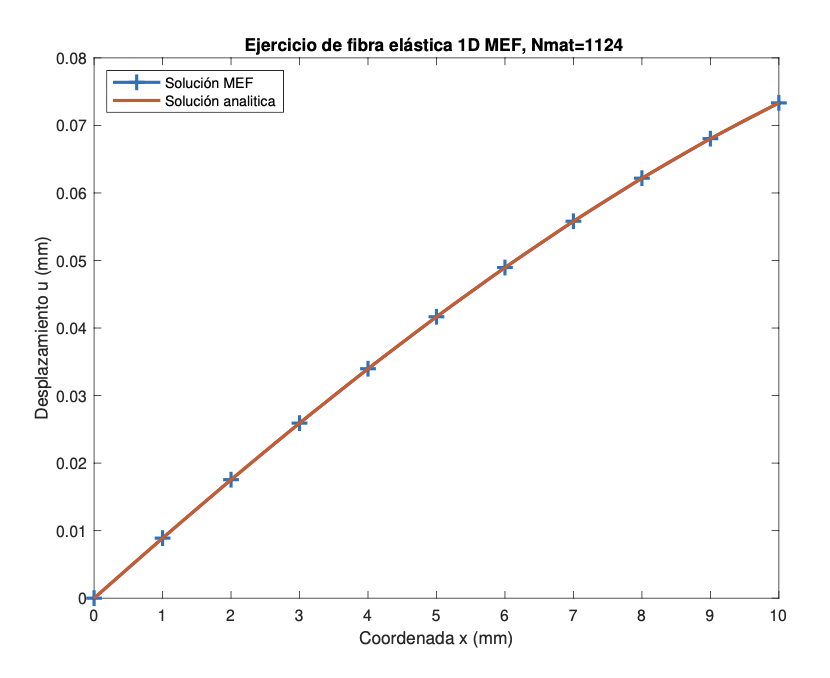
\includegraphics[width=0.5\textwidth]{figuras/u-matlab.png}%
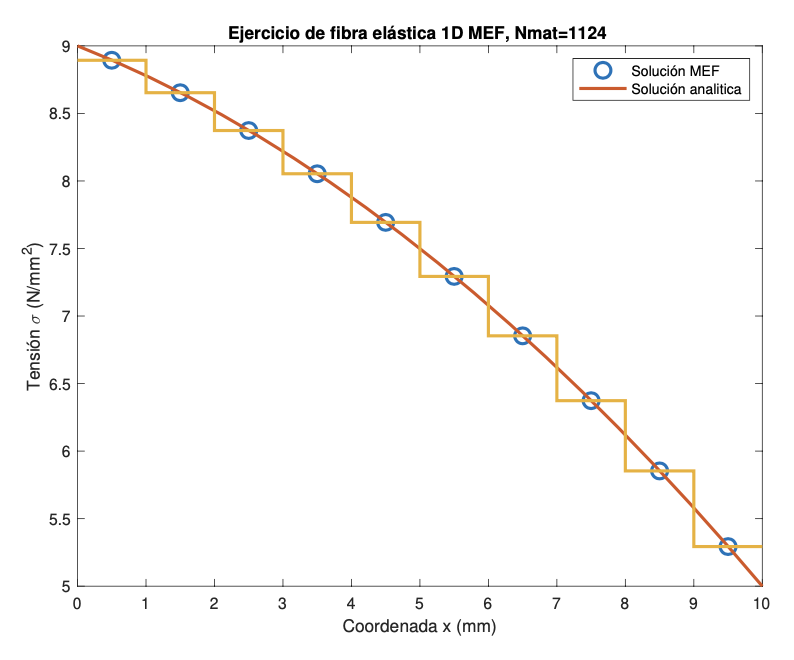
\includegraphics[width=0.5\textwidth]{figuras/s-matlab.png}
%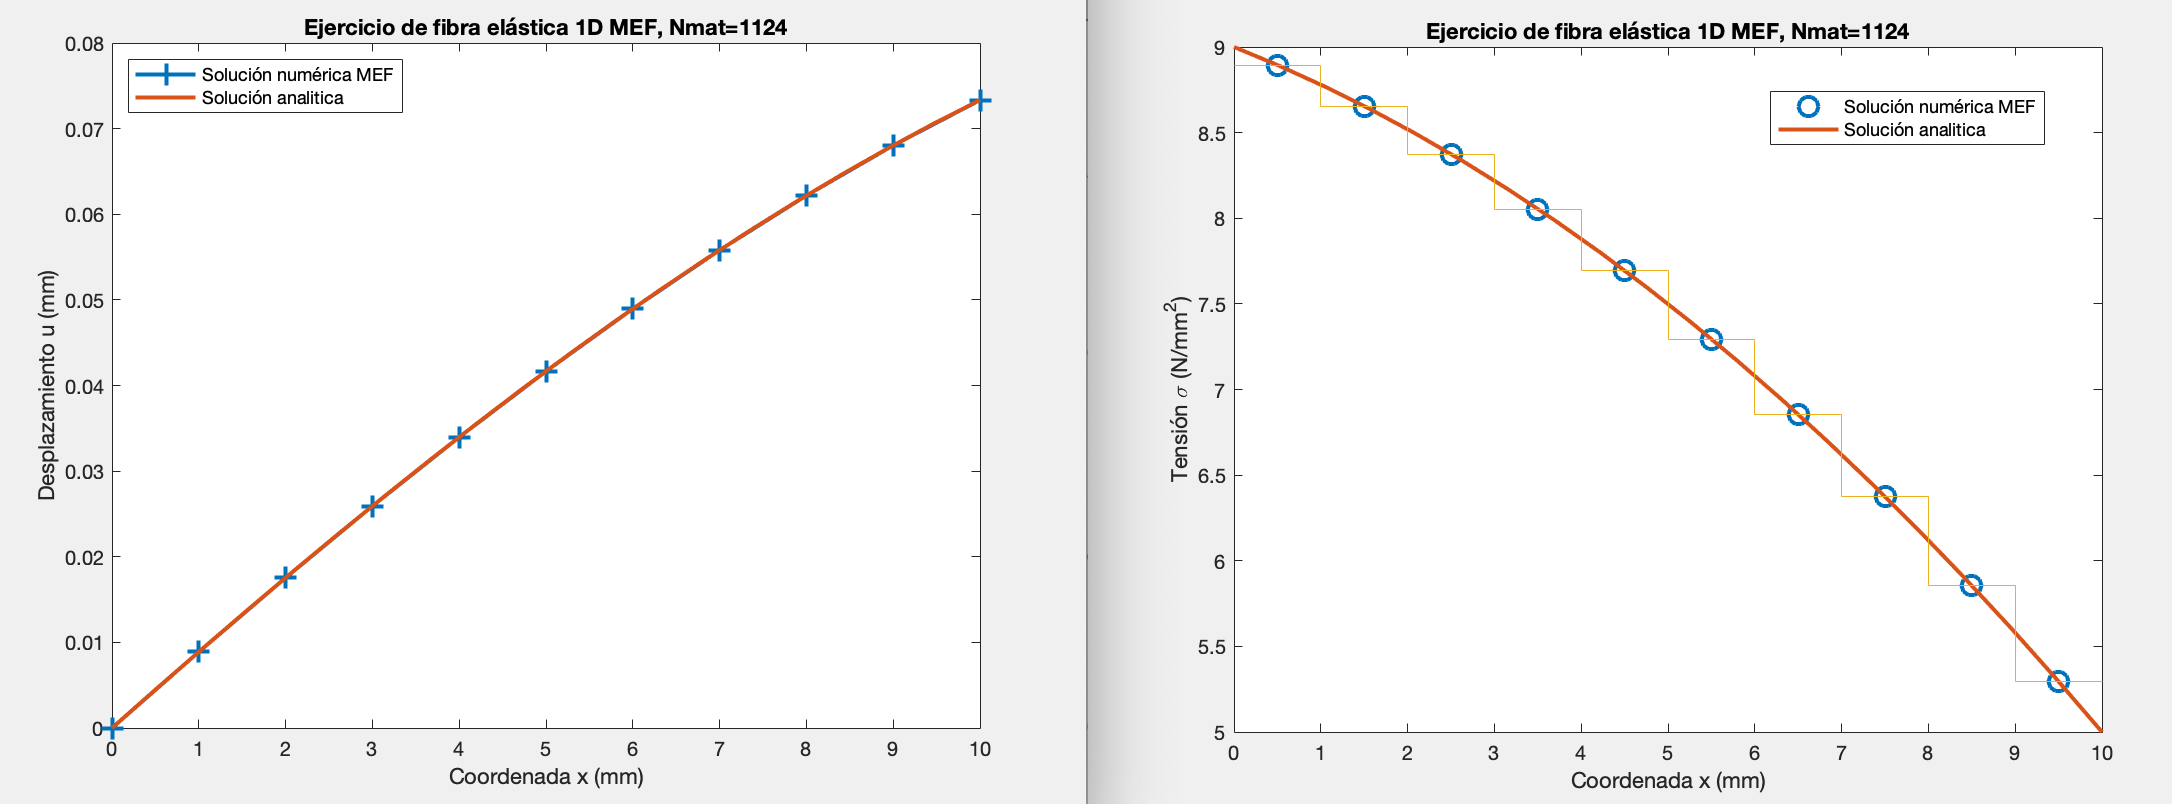
\includegraphics[scale=0.45]{capturas/sol_matlab.png}
\caption{Comparison between the solution in MatLab and the analytical solution.}
\label{fig:solmatlab}
\end{figure}

\item Comparison between \texttt{MatLab} / \texttt{Octave} and the analytical solution

We prepare the \texttt{MatLab} / \texttt{Octave} code to also plot the result that we saved from \emph{Abaqus}:

\begin{lstlisting}[ label=codigo5,caption=Scheme Matlab-Abaqus]
% E: ABAQUS
%----------------------------------------------------------------

xn_ab=[

    ]; 

un_ab=[

    ];

xe_ab=[                      

    ];

sigma_ab=[

    ];

% % 1. Plot displacements in x
figure 
plot(xn_ab,un_ab,'-+',xc,uc,'-','LineWidth',2,'MarkerSize',10)
%hold
title(['Study of a 1D elastic fibre, Nmat=' num2str(Nmat)]);
legend({'FE Solution with Abaqus','Analytical solution'},'Location','Northwest')
xlabel('Coordinate x (mm)');
ylabel('Displacement u (mm)');

% 3.2. Plot the stress along the bar (x)
figure
plot(xe_ab,sigma_ab,'o',xc,sigmac,'-','LineWidth',2,'MarkerSize',10)
hold
xs=linspace(L,0,Nele+1);
stairs(xs,[sigma_ab;sigma_ab(Nele)],'LineWidth',2)
title(['Study of a 1D elastic fibre, Nmat=' num2str(Nmat)]);
legend({'FE Solution with Abaqus','Analytical solution'},'Location','Northwest');
xlabel('Coordinate x (mm)');
ylabel('Stress \sigma (N/mm^2)');
\end{lstlisting}

Figure \ref{fig:out3} shows the results obtained running this code. It can be observed that the result is identical with the FE code in Matlab (figura~\ref{fig:solmatlab}) and that in Python, and they coincide with the exact analytical value at the nodes for displacements, and at the middle of the elements for the stresses. 

% ACC Python or abaqus?

\begin{figure}[h!tp]
\centering
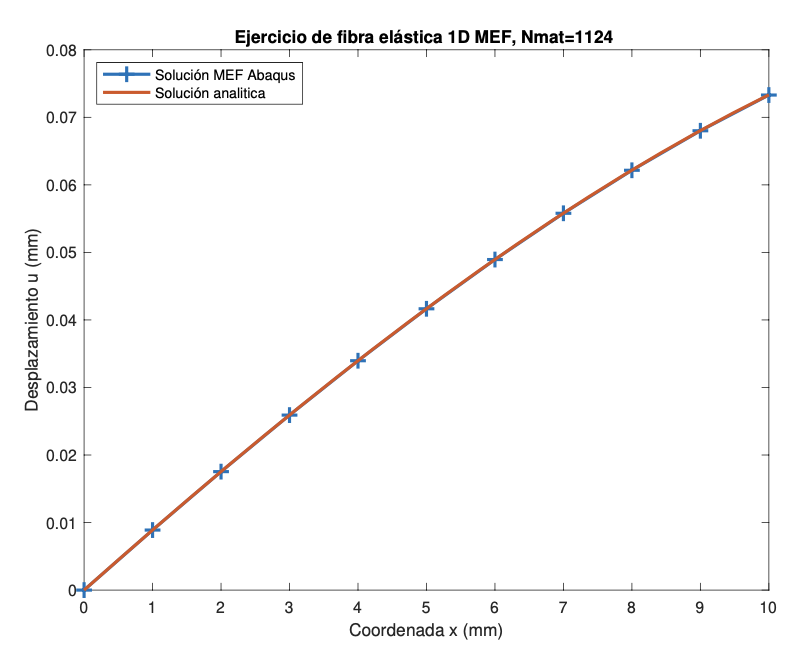
\includegraphics[width=0.5\textwidth]{figuras/u-abaqus.png}%
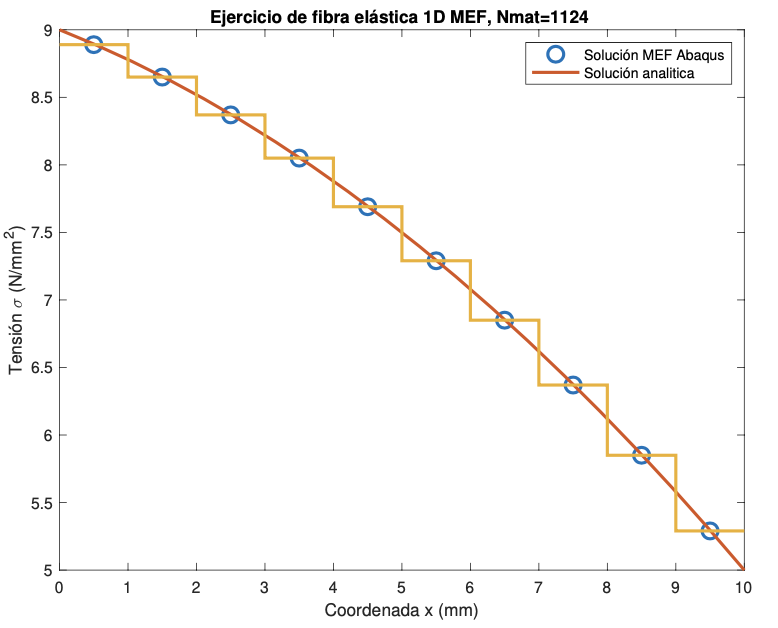
\includegraphics[width=0.5\textwidth]{figuras/s-abaqus.png}
%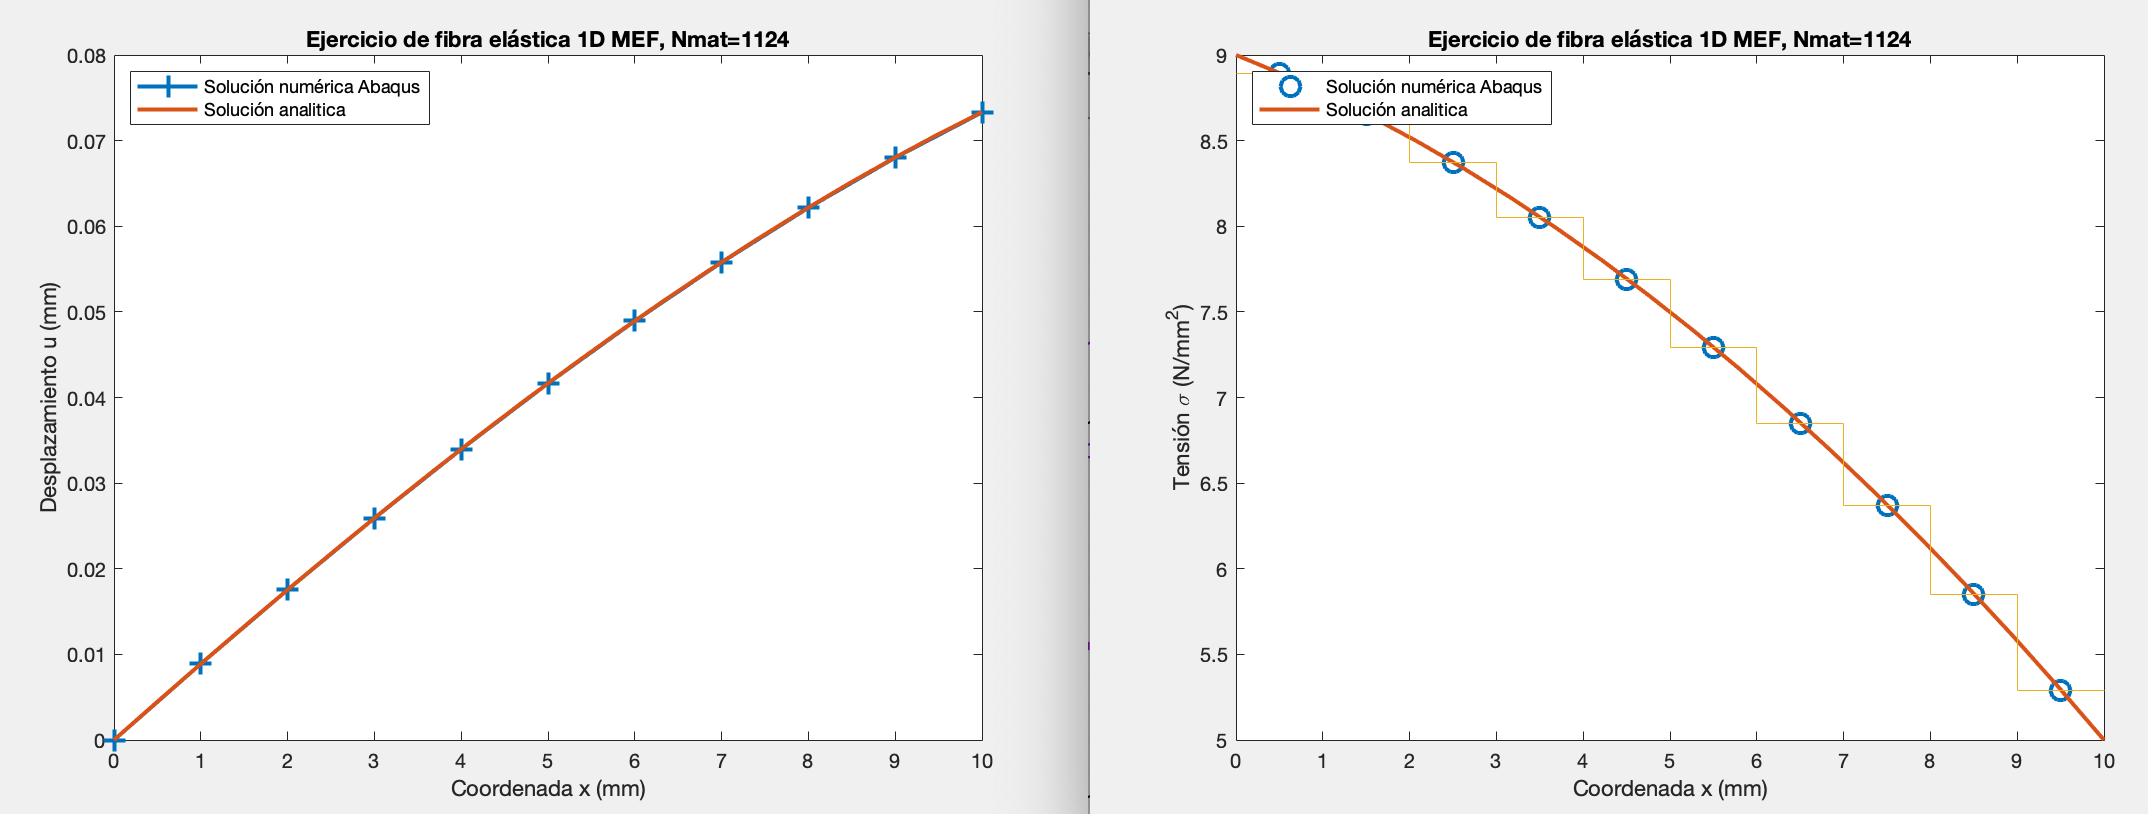
\includegraphics[scale=0.45]{capturas/out3.png}
\caption{Comparison between the analytical solution and the FE solution in \emph{Abaqus}.}
\label{fig:out3}%
\end{figure}

\end{itemize}
%\begin{thebibliography}{10}
%\end{thebibliography}

\end{document}
